%% 
%% Copyright 2007-2024 Elsevier Ltd
%% 
%% This file is part of the 'Elsarticle Bundle'.
%% ---------------------------------------------
%% 
%% It may be distributed under the conditions of the LaTeX Project Public
%% License, either version 1.3 of this license or (at your option) any
%% later version.  The latest version of this license is in
%%    http://www.latex-project.org/lppl.txt
%% and version 1.3 or later is part of all distributions of LaTeX
%% version 1999/12/01 or later.
%% 
%% The list of all files belonging to the 'Elsarticle Bundle' is
%% given in the file `manifest.txt'.
%% 
%% Template article for Elsevier's document class `elsarticle'
%% with numbered style bibliographic references
%% SP 2008/03/01
%% $Id: elsarticle-template-num.tex 249 2024-04-06 10:51:24Z rishi $
%%
\documentclass[preprint,12pt]{elsarticle}

%% Use the option review to obtain double line spacing
%% \documentclass[authoryear,preprint,review,12pt]{elsarticle}

%% Use the options 1p,twocolumn; 3p; 3p,twocolumn; 5p; or 5p,twocolumn
%% for a journal layout:
%% \documentclass[final,1p,times]{elsarticle}
%% \documentclass[final,1p,times,twocolumn]{elsarticle}
%% \documentclass[final,3p,times]{elsarticle}
%% \documentclass[final,3p,times,twocolumn]{elsarticle}
%% \documentclass[final,5p,times]{elsarticle}
%% \documentclass[final,5p,times,twocolumn]{elsarticle}

%% For including figures, graphicx.sty has been loaded in
%% elsarticle.cls. If you prefer to use the old commands
%% please give \usepackage{epsfig}

%% The amssymb package provides various useful mathematical symbols
\usepackage{amssymb}
%% The amsmath package provides various useful equation environments.
\usepackage{amsmath}
\usepackage{xcolor}
%% The amsthm package provides extended theorem environments
%% \usepackage{amsthm}

%% The lineno packages adds line numbers. Start line numbering with
%% \begin{linenumbers}, end it with \end{linenumbers}. Or switch it on
%% for the whole article with \linenumbers.
%% \usepackage{lineno}

\usepackage{booktabs}
\usepackage{multirow}
\usepackage{bm}
\usepackage[a4paper,margin=2.5cm]{geometry}
\usepackage{amsmath,amssymb}
\usepackage[ruled,vlined,linesnumbered]{algorithm2e}
\usepackage{makecell}
\usepackage{graphicx}
\usepackage{subcaption}

\journal{Knowledge-Based Systems}

\begin{document}

\begin{frontmatter}

%% Title, authors and addresses

%% use the tnoteref command within \title for footnotes;
%% use the tnotetext command for theassociated footnote;
%% use the fnref command within \author or \affiliation for footnotes;
%% use the fntext command for theassociated footnote;
%% use the corref command within \author for corresponding author footnotes;
%% use the cortext command for theassociated footnote;
%% use the ead command for the email address,
%% and the form \ead[url] for the home page:
\title{A Variational Gaussian Mixture Framework with Anatomical Priors for Unsupervised Cardiac Segmentation\tnoteref{label1}}

\tnotetext[label1]{This work was supported in part by the National Natural Science Foundation of China
(Grant No. 62201355, 62071303), Guangdong Basic and Applied Basic Research Foundation
(2024A1515010977), Shenzhen Science and Technology Project (JCYJ20220531102407018), Guangdong Provincial Key Laboratory (Grant 2023B1212060076).}
\author{Youwei Peng, Jiajun Zhao,  Xuan Yang\fnref{label2}}
\ead{yangxuan@szu.edu.cn}
%\ead[url]{home page}
\fntext[label2]{Corresponding author}
%\cortext[cor1]{}
% \affiliation{organization={},
%             addressline={},
%             city={},
%             postcode={},
%             state={},
%             country={}}

%\title{}

%% use optional labels to link authors explicitly to addresses:
%% \author[label1,label2]{}
%% \affiliation[label1]{organization={},
%%             addressline={},
%%             city={},
%%             postcode={},
%%             state={},
%%             country={}}
%%
%% \affiliation[label2]{organization={},
%%             addressline={},
%%             city={},
%%             postcode={},
%%             state={},
%%             country={}}

%\author{} %% Author name

%% Author affiliation
\affiliation{organization={College of Computer Science and Software Engineering, Shenzhen University},%Department and Organization
            addressline={Nanhai Ave.3688}, 
            city={Shenzhen},
            postcode={518060}, 
            state={Guangdong},
            country={China}}

%% Abstract
\begin{abstract}
%% Text of abstract
Accurate cardiac segmentation is crucial for quantitative assessment of cardiac diseases. However, existing supervised and semi-supervised methods heavily rely on annotated data and often struggle with limited labeled data and cross-domain generalization. In this paper, we propose VGM-Seg, an unsupervised cardiac segmentation framework based on a variational Gaussian mixture model (GMM). 
We model pixel-wise image features explicitly using the variational GMM by introducing latent variables representing Gaussian assignment weights and derive the corresponding evidence lower bound (ELBO) for variational inference. 
An anatomical prior is incorporated to generate a sample-specific dynamic prior, which regularizes the posterior distributions of the latent variables. 
Three dedicated subnetworks are jointly trained to estimate the Gaussian parameters, their concentration weights, and soft segmentation labels. 
By integrating explicit anatomical knowledge into the variational GMM, the sample-specific dynamic prior effectively enhances cross-domain generalization without requiring labeled data. 
Extensive experiments on four public datasets demonstrate that VGM-Seg achieves robust cross-domain performance and outperforms representative semi-supervised segmentation methods under limited labeled data.

\end{abstract}

%%Graphical abstract
\begin{graphicalabstract}
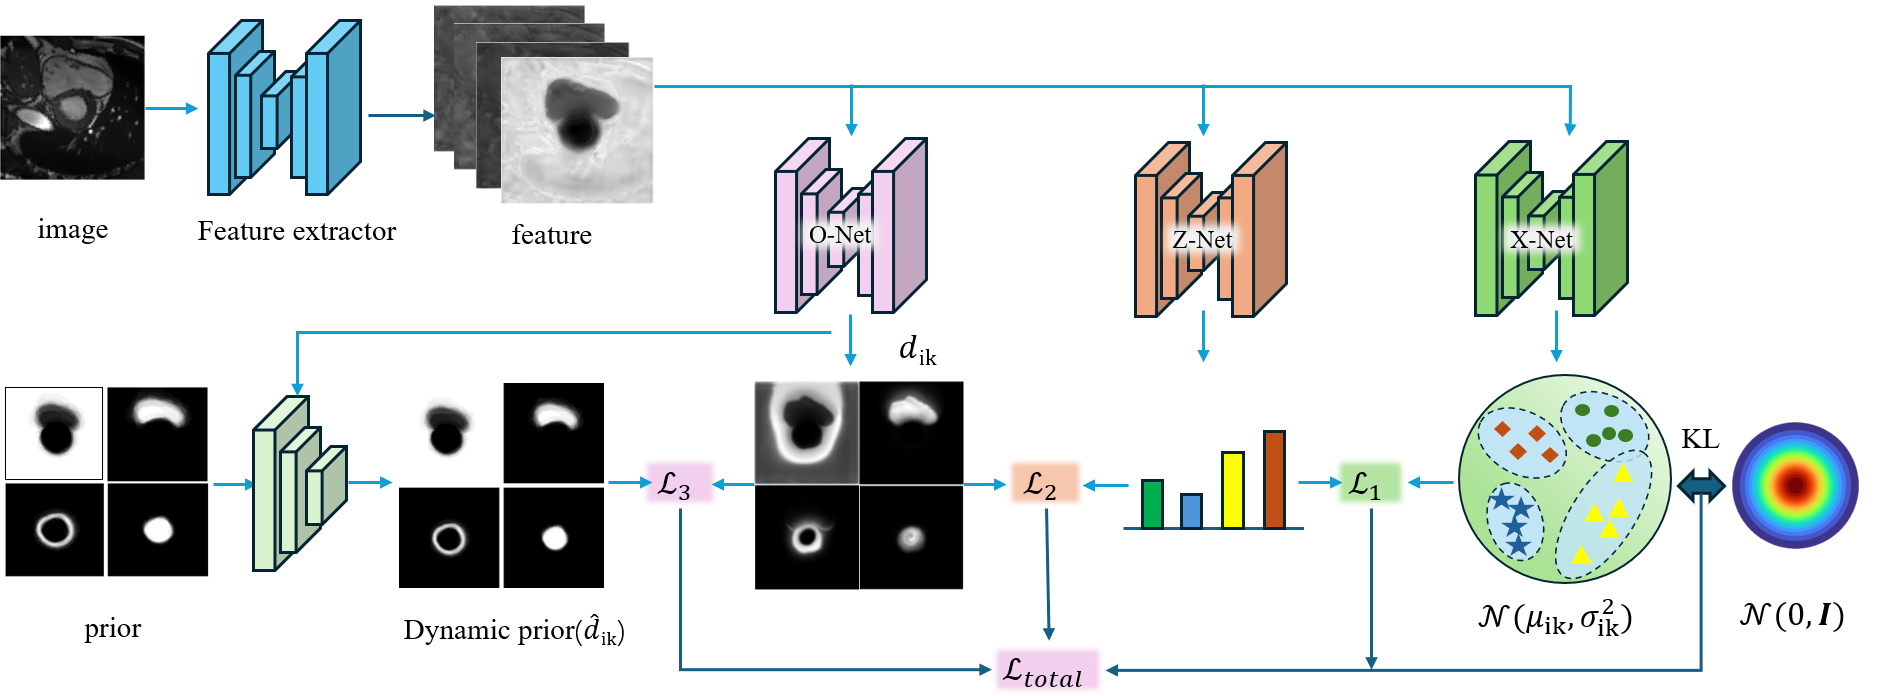
\includegraphics[width=1\linewidth]{Image/framework.png}
\end{graphicalabstract}

%%Research highlights
\begin{highlights}
\item We propose an unsupervised cardiac segmentation framework based on a variational Gaussian mixture model.
\item An anatomical prior is constructed, and a sample-specific dynamic prior is further generated via a registration model to improve cross-domain generalization.
\item Three sub-networks are jointly trained under the derived ELBO objective to estimate Gaussian parameters, mixture concentration weights, and soft segmentation labels.
\end{highlights}

%% Keywords
\begin{keyword}

Unsupervised Cardiac Segmentation \sep  Variational Inference \sep Gaussian Mixture Model \sep Anatomical Prior \sep Cross-domain
\end{keyword}

\end{frontmatter}


%
\section{Introduction}

Accurate cardiac image segmentation is essential for cardiac quantitation in clinical applications. It provides the foundation for assessing cardiac morphology and function, such as ventricular volume, myocardial mass, ejection fraction, and regional wall-motion abnormalities~\cite{song2022deep,alabed2022quality}, which are critical for diagnosis, prognosis, and therapeutic decision-making.

Deep learning-based segmentation methods have demonstrated remarkable performance. 
According to the annotated data used in segmentation models, cardiac image segmentation can be broadly categorized into fully supervised, semi-supervised, and unsupervised learning methods. 
Fully supervised methods rely on labeled data and optimize loss functions such as cross-entropy or Dice to measure the discrepancy between predictions and ground-truth labels~\cite{unet,Bernard2018Deep,chang2022deeprecon}. However, due to the scarcity and high acquisition cost of expert-annotated cardiac images, applications of fully supervised methods are limited in real-world clinical scenarios.
%Sparse annotation
Weakly supervised learning relies on incomplete, inexact, or noisy labels instead of dense ground-truth annotations, such as the scribble-guided method~\cite{zhang2022shapepu,zhuang2022cardiac} that requires only sparse annotation with weak supervision of scribbles.

Semi-supervised learning (SSL) uses a small amount of fully labeled data together with a large amount of unlabeled data through consistency regularization~\cite{WANG2025104341}, teacher-student training~\cite{tarvainen2017mean,yu2019uncertainty,DC-Net,QIU2025108613}, pseudo-label-based self-training~\cite{cps,CHAITANYA2023102792,SS-Net,ALHVR,LYU2023120836,YU2024106145}, and generative learning~\cite{DECOURT2020103884}.
%
%
However, SSL still assumes a non-trivial amount of target-domain annotations and may degrade under domain shifts across vendors, protocols, and patient populations~\cite{Campello2021Multi}. Therefore, stable segmentation in the fully label-free unsupervised setting remains a challenge.



Unsupervised methods are fully label-free and classify objects by clustering or probabilistic models, atlas priors, feature alignment, or self-supervised representation learning.
Unsupervised approaches such as Gaussian mixture model (GMM) are classical probabilistic models that represent complex data distributions as a weighted combination of multiple Gaussian components. GMM captures multi-modal feature distributions and explicitly quantifies uncertainty through probabilistic inference. Due to their statistical foundation, GMM provides an interpretable and flexible framework for unsupervised segmentation.
However, traditional GMM lacks representation learning capabilities and is typically a probabilistic model that exhibits limited robustness to domain shifts~\cite{tuia2016domain}.



In this paper, our method formulates unsupervised cardiac image segmentation as variational inference under a pixel-wise GMM, while explicitly incorporating anatomical priors to regularize cross-domain learning. Unlike existing GMM based on classical EM, we integrate deep feature learning, variational inference, and anatomical priors into a unified framework.
Integrating variational Gaussian mixture models with deep neural networks enables expressive feature representations, effectively bridging statistical interpretability and deep representation learning in a fully unsupervised manner.
Specifically, variational inference enables scalable and stable optimization of GMM parameters within deep networks, quantifying crucial uncertainty for reliable cardiac image analysis.
The soft assignment of GMM naturally accommodates ambiguous anatomical boundaries, and the probabilistic formulation provides a natural interface for incorporating anatomical priors, enabling robust cross-domain generalization without explicit domain alignment.



We propose an unsupervised cardiac segmentation model that integrates a variational Gaussian mixture model with deep neural networks, denoted as VGM-Seg. 
%
We derive an evidence lower bound (ELBO) for the variational GMM and construct a statistical cardiac anatomical prior from a small auxiliary labeled dataset. The sample-specific dynamic prior is generated via a pre-trained registration network, regularizing the estimated posterior in the target domain without any target labels. 
Three sub-networks are optimized to jointly estimate the Gaussian distribution parameters, their concentration weights, and soft segmentation labels, respectively. 


Compared with unsupervised domain adaptation methods that leverage annotated source-domain data and unannotated target-domain data, our VGM-Seg is a fully unsupervised model on both the source and target domains. Although retraining is required when adapting to a new domain, our VGM-Seg is fundamentally different from semi-supervised or domain adaptation methods.


%
To the best of our knowledge, our work is the first work to formulate unsupervised cardiac image segmentation as variational inference under a Gaussian mixture modeling framework.
%
Our main contributions are summarized as follows:
\begin{itemize}
  \item We propose an unsupervised cardiac segmentation framework, which is based on variational GMM in image feature space to estimate mixture weights and Gaussian parameters, enabling fully label-free segmentation.
  \item We design a Dirichlet anatomical prior and an alignment strategy to generate a sample-specific dynamic prior via a rigid registration module. The dynamic prior is different for different samples and evolves continuously during training, serving as an important constraint on the posterior in the variational GMM framework.
  \item Experiments on four public datasets show that, in a fully unsupervised setting, our VGM-Seg outperforms representative semi-supervised methods trained with 5\%-10\% labeled data, and shows strong cross-domain generalization compared with unsupervised domain adaptation methods.
\end{itemize}


\section{Related Work}

In the absence of labeled data, unsupervised image segmentation methods aim to delineate object structures using intrinsic image characteristics, anatomical priors, or statistical modeling assumptions. Existing approaches can be broadly categorized according to their underlying principles, including clustering or probabilistic model–based methods, atlas or prior-guided approaches, feature alignment–based methods, as well as self-supervision–based strategies. 

%
\textbf{Clustering or probabilistic models-based} methods group pixel-wise features based on statistical similarity. Representative approaches include K-means or fuzzy C-means~\cite{pham2002adaptive}, Gaussian mixture model (GMM)~\cite{bishop2006pattern}, hidden Markov random fields~\cite{fan2020unsupervised}, or variational Bayesian spatial mixture models~\cite{woolrich2006variational}.


%For spatial mixture models that used
% discrete Markov random field (MRF) priors, Woolrich \textit{et al.}~\cite{woolrich2006variational} employed a variational Bayes approximation with an order of magnitude faster than MCMC.
%
The traditional GMM model tissue intensity distributions enable unsupervised segmentation.
However, traditional GMM is sensitive to variations in noise and domain due to its limited representation ability. 
With the development of deep learning, GMM has been integrated with deep neural networks, giving rise to deep GMM-based frameworks with enhanced representational capacity.
Liang \textit{et al.}~\cite{liang2022gmmseg} built a GMM to model the data distribution of each class in the feature space via Expectation-Maximization (EM), to capture class-conditional densities. It learned generative classification with end-to-end discriminative representation compactly and collaboratively. 
%
Schwab \textit{et al.}~\cite{deepGMM} minimized the negative log-likelihood (NLL) function with respect to GMM to estimate GMM parameters using a convolutional neural network (CNN) through EM. 
%
Naseer \textit{et al.}~\cite{naseer2024multimodal} extracted spatial attributes and segmented multi-object using the GMM technique with a multi-layer perceptron architecture. 
%
Pu \textit{et al.}~\cite{pu2023deep} designed a deep expectation-maximization (DEM) network by modeling an image in its latent feature space using a GMM, jointly learning the latent features of the image and the GMM model of the latent features in a single framework. 

%
\textbf{Atlas priors-based} methods relied on anatomical templates and deformable registration to propagate structural atlases or priors to target images~\cite{zhou2017cardiac,milo2022atlas,finnegan2023open,chin2023validation}. 
% 
%
The shape prior is generally constructed by computing the empirical proportion in pixels of each class based on the field of ground truth labels~\cite{zotti2018convolutional,li2021semi}.
%
Huang \textit{et al.}~\cite{huang2021medical} integrated the medical image anatomical prior using probabilistic atlas into deep learning models by incorporating the prior loss with conventional likelihood losses.
%
Painchaud \textit{et al.}~\cite{painchaud2020cardiac} trained an adversarial variational autoencoder to generate a latent space of cardiac statistical shape from mask images and project any implausible shape into
the cardiac latent space and steer it toward the closest correct shape.
Gilbert \textit{et al.}~\cite{gilbert2020artificial} indicated that a dynamic atlas that models changes in cardiac shape deformation, myocardial strain, and strain rate will be a fruitful area of future research. 
%
Atlas priors-based methods ensure anatomical plausibility but are highly dependent on atlas quality and registration accuracy, limiting generalization across domains.

%
\textbf{Feature alignment-based} methods learn domain-invariant feature representations by aligning feature distributions across different domains employing adversarial training~\cite{zheng2025unsupervised,sun2022rethinking,zhang2023st,wang2022unsupervised} or feature-level alignment~\cite{feng2023unsupervised} to enforce similarity between source and target feature spaces. They can be generalized from labeled source-domain data to unlabeled target-domain data, which are effective for cross-domain and domain adaptation scenarios.
%
Feng \textit{et al.} indicated that most existing adversarial training may still produce overconfident but erroneous results on unseen target images. They aligned the semantic of the cross-modality images to perform a class-level distribution adaptation.
%
To reduce the difference in distribution between the two domains, Cui \textit{et al.}~\cite{cui2024toward} aligned posterior distributions of the two domains using the variational autoencoder (VAE).
%
Disentanglement learning factorizes an image into domain-invariant anatomy and domain-specific modality components, which has been used in domain adaptation.
Sun \textit{et al.}~\cite{sun2022attention} aligned coarse features at the image-level and removed the remaining fine domain shift using channel disentangled representation learning.  
 

%evalution
Zhuang \textit{et al.}~\cite{zhuang2022cardiac} evaluated three unsupervised methods~\cite{chen2019unsupervised,wang2019multi,ly2019style} for cardiac image segmentation. One of them adopted the label information that came from the source domain, and the target domain images do not have a label. 
The other two methods used labeled images for pretraining and then fine-tuned the networks with limited labeled images. 
They noted that there are no obvious differences in segmentation performance between these methods and that the domain shift is required to be marginal.
%
In general, these feature alignment-based methods may degrade performance when large domain discrepancies or complex anatomical variations are present.


%
\textbf{Self-supervised representation learning} methods aim to provide deep feature learning without large annotated datasets, thus alleviating the annotation bottleneck~\cite{ericsson2022self}. 
They learn feature embeddings from unlabeled data through reconstruction~\cite{chang2022deeprecon,lu2022unsupervised} or contrastive learning~\cite{gu2024unsupervised,qiao2024cmrvae}, followed by clustering or post-processing for segmentation~\cite{bai2019self}.
%
Xie \textit{et al.}~\cite{xie2022unsupervised} further employed a self-training strategy for the target domain through adversarial learning and pseudo-label, which implicitly facilitates feature alignment in the anatomy space.
%
Wen \textit{et al.}~\cite{wen2022self} simultaneously optimized the two coupled objectives of semantic grouping and contrastive learning, showing advantages over hand-crafted priors and being able to learn object-level representations. 
%
To overcome the limitation of self-supervised learning that relies on large-scale datasets, Nguyen \textit{et al.}~\cite{nguyen2025matssl} perform self-supervised pretraining on a small-scale, unlabeled dataset and then fine-tune the model on multiple benchmark datasets. 
%
%
Soltanieh \textit{et al.}~\cite{soltanieh2023distribution} evaluated the performance of popular self-supervised methods in various ECG-based arrhythmia datasets and assessed their generalizability. They showed that self-supervised learning enhances the performance of ECG-based diagnostic systems. 



\section{Method}

\subsection{Variational Gaussian Mixture Model}

A Gaussian mixture model (GMM) is a universal approximation for continuous probability densities, implying that it can approximate any target distribution arbitrarily well given a sufficient number of components.
%
For image segmentation, GMM models pixel-wise features with $K$ Gaussian distributions to represent complex and multi-modal feature distributions, yielding soft class assignments and uncertainty estimates.

In this paper, we construct a pixel-wise GMM in the image feature space rather than the intensity space to model the distribution of image features. 
We employ a simple U-Net to extract image features. The U-Net is pre-trained using a limited amount of labeled data, which is the same set of annotations used for anatomical prior construction in our model.
%
It should be emphasized that the labeled data we used were only for anatomical prior construction and a pre-trained feature extractor, which is applied during training on different domain datasets. In other words, regardless of which dataset is used for training, the labeled data remain fixed and do not change.

Figure~\ref{fig:gaussian} presents the statistical histograms of image features across each dimension, together with the histogram of image intensity. 
The feature histograms are shown in the first row and in the bottom-left of the second row, whereas the image intensity histogram is displayed in the bottom-right corner. Each histogram is overlaid with its corresponding Gaussian fitting curve. 
It can be observed that the feature distributions corresponding to specific classes are compact and well separated in at least one feature dimension, such as the left ventricle (LV) feature shown in the second panel of the first row, which can be approximated by Gaussian distributions.
%
This phenomenon demonstrates the advantage of employing a feature extractor pre-trained for segmentation. Such a feature extractor does not need to achieve good segmentation performance; rather, it only needs to have a certain level of inter-class feature separability. Consequently, even using a limited amount of annotated data, it is sufficient to promote intra-class feature compactness and inter-class feature discrimination.
%
In contrast, the image intensity distributions are heavily overlapped, especially between the background and objects, making it challenging to distinguish the background from the objects only on the basis of image intensity.


\begin{figure}[htpb]
  \centering
  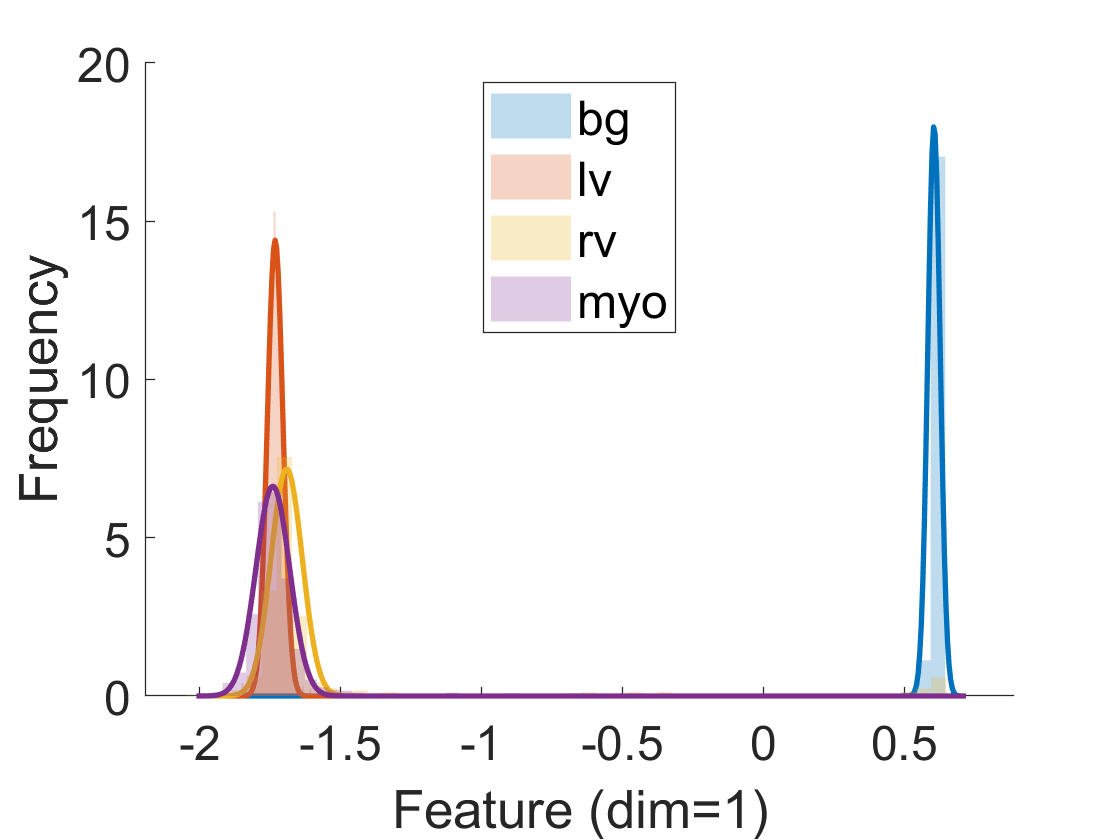
\includegraphics[width=0.32\linewidth]{Image/hist0.png}
  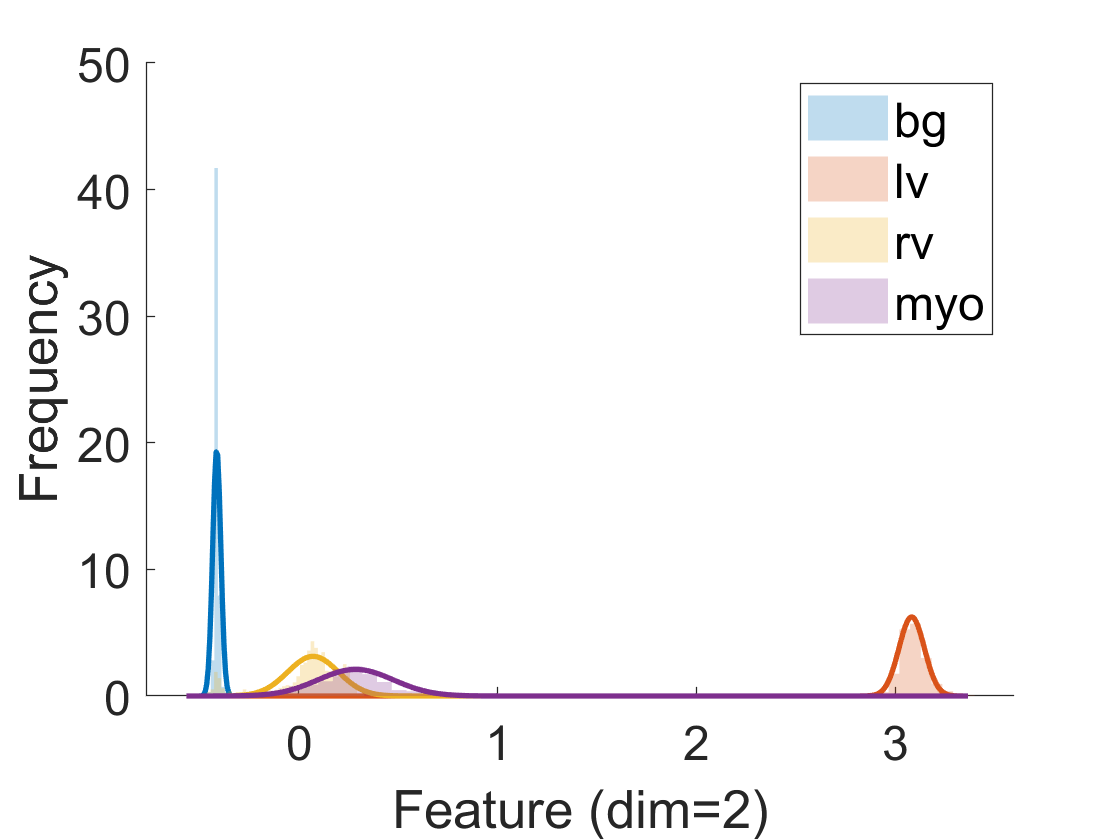
\includegraphics[width=0.32\linewidth]{Image/hist1.png}
  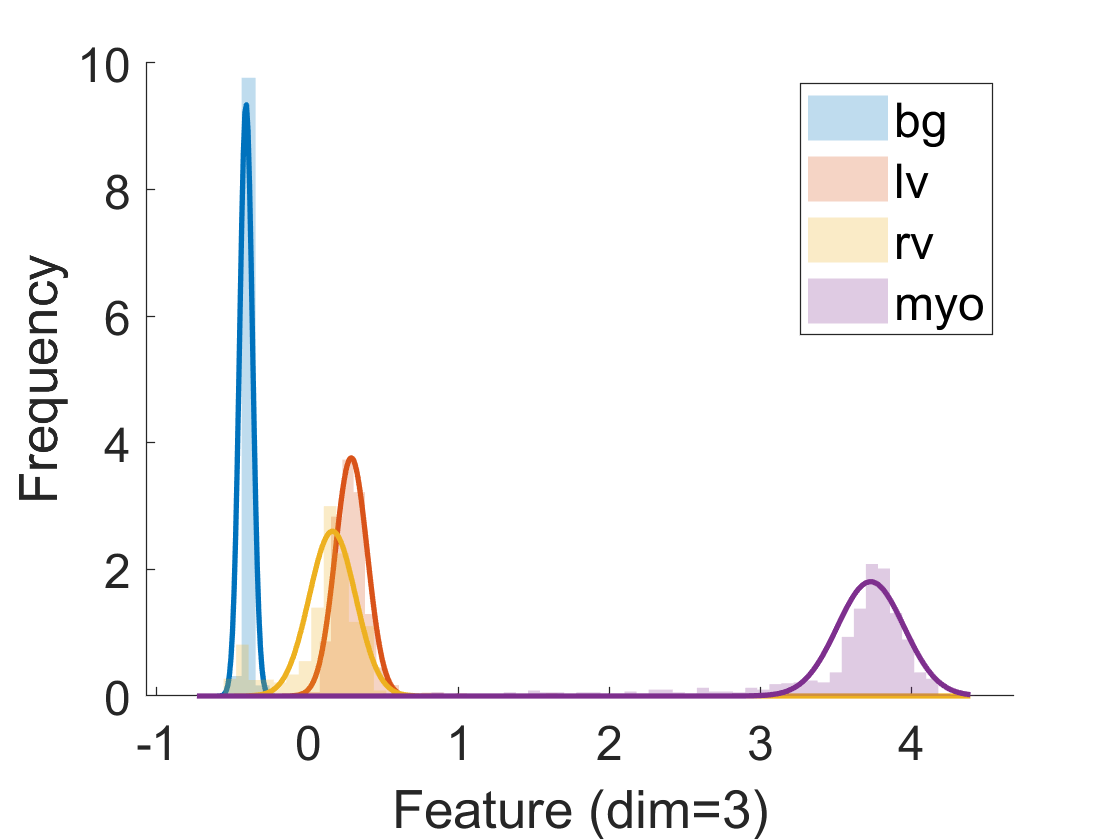
\includegraphics[width=0.32\linewidth]{Image/hist2.png}
  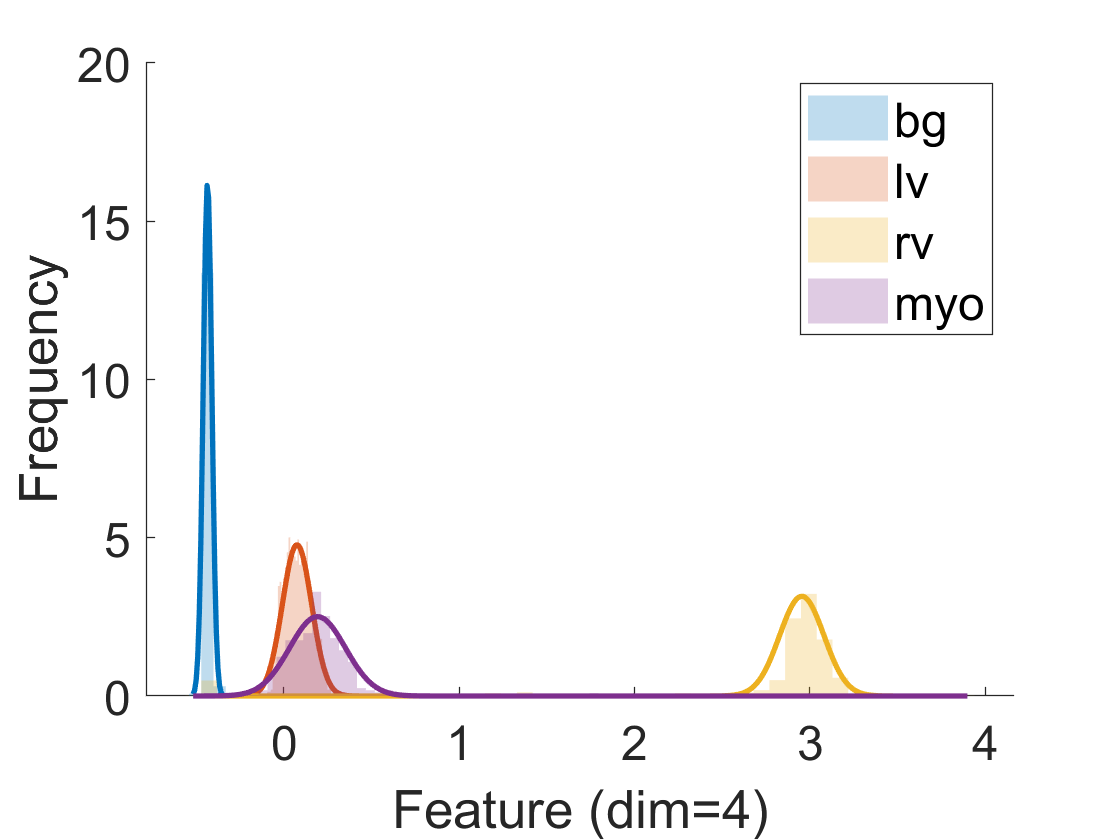
\includegraphics[width=0.32\linewidth]{Image/hist3.png}
  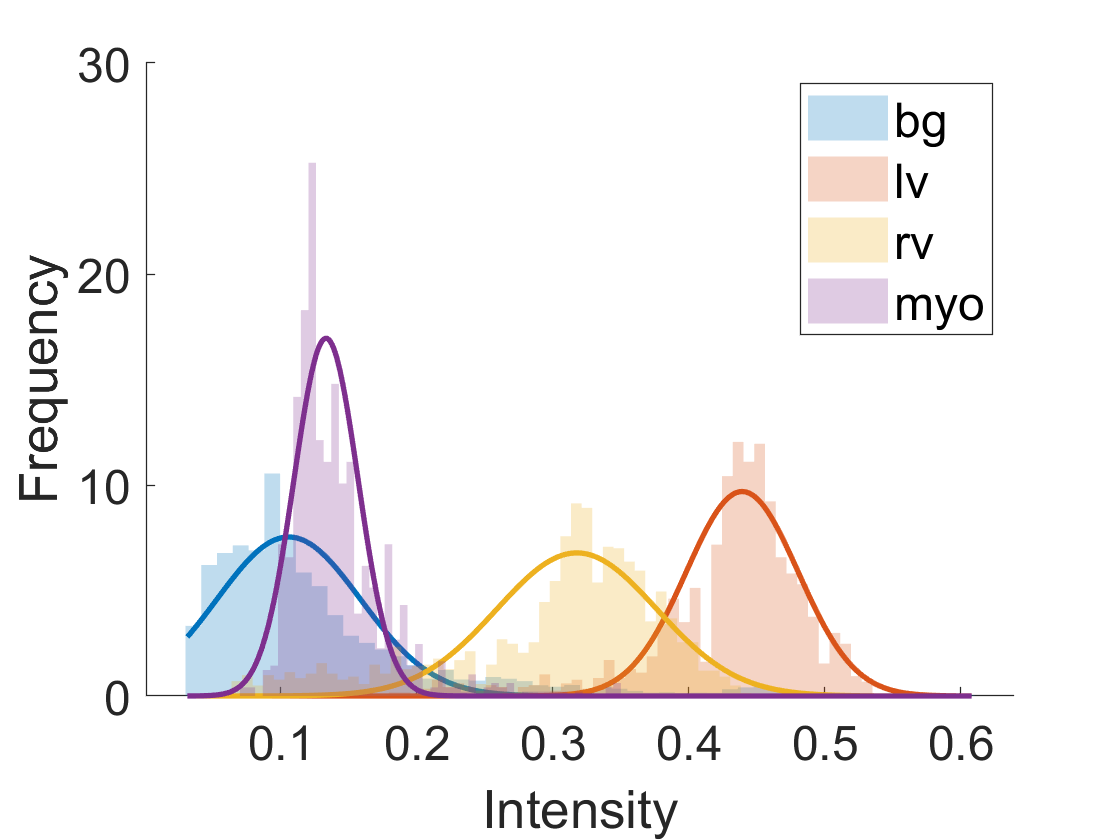
\includegraphics[width=0.32\linewidth]{Image/histImg.png}
  \caption{Statistical histograms of features across each dimension and image intensity. The feature histograms occupy the top row and the bottom-left panel, while the intensity histogram is shown in the bottom-right panel. Gaussian fitting curves are overlaid on each histogram. Dimensions 1–4 correspond to the background (BG), left ventricle (LV), myocardium (MYO), and right ventricle (RV), respectively.}
  \label{fig:gaussian}
\end{figure}



Given an image $X$ with $N$ pixels, let $\mathbf{x}_i \in \mathbb{R}^d$ denote the feature of the $i$-th pixel extracted by a trained network.
All features of $X$ are $\mathbf{x}=\{\mathbf{x}_i\}_{i=1}^N$. 
GMM assumes that each $\mathbf{x}_i$ is generated by the linear combination of $K$ Gaussian components as

\begin{equation}
\label{likelihood}
p(\mathbf{x}_i) = \sum_{k=1}^{K} \omega_{ik} \, \mathcal{N}(\mathbf{x}_i \mid \boldsymbol{\mu}_{ik}, \boldsymbol{\sigma}^2_{ik}), \qquad
\sum_{k=1}^{K} \omega_{ik} = 1
\end{equation}
where $K$ is the class number, 
$\boldsymbol{\mu}_{ik}$ and $\boldsymbol{\sigma}^2_{ik}$ are the mean vector and (diagonal) variance vector of the $k$-th Gaussian component, i.e., with covariance $\mathrm{diag}(\boldsymbol{\sigma}^2_{ik})$. $\omega_{ik}$ is the corresponding Gaussian mixture weight. 
In the following, symbols without subscripts denote the collection of all corresponding elements.


We propose a model, denoted VGM-Seg, by combining variational inference with GMM for medical segmentation. 
A discrete assignment latent variable $\mathbf{z}_i = (z_{i1}, \dots, z_{iK})$ is introduced for the $i$-th pixel, where $z_{ik} \in \{0,1\}$ and $\sum_{k=1}^{K} z_{ik} = 1$. 
%
Given a sample of $\mathbf{z}_i$, only the Gaussian component with $z_{ik} = 1$ contributes to the likelihood

\begin{equation}
\label{likelihood-prod}
p(\mathbf{x}_i \mid \mathbf{z}_i) =
\prod_{k=1}^{K}
\mathcal{N}(\mathbf{x}_i \mid \boldsymbol{\mu}_{ik}, \boldsymbol{\sigma}^2_{ik})^{z_{ik}}.
\end{equation}
%
It is assumed that the $\mathbf{z}_i$ follows a categorical distribution with the parameter $\omega_{ik}$,
\begin{equation}
p(\mathbf{z}_i) = \prod_{k=1}^{K} \omega_{ik}^{z_{ik}}.
\end{equation}
Then, the joint distribution of $p(\mathbf{x}_i, \mathbf{z}_i)$ is

\begin{equation}
p(\mathbf{x}_i, \mathbf{z}_i) =
\prod_{k=1}^{K}
\left[
\omega_{ik} \, \mathcal{N}(\mathbf{x}_i \mid \boldsymbol{\mu}_{ik}, \boldsymbol{\sigma}^2_{ik})
\right]^{z_{ik}}.
\end{equation}
%
Marginalizing over $\mathbf{z}_i$ of $p(\mathbf{x}_i, \mathbf{z}_i )$ yields $\sum_{\mathbf{z}_i} p(\mathbf{x}_i, \mathbf{z}_i) = p(\mathbf{x}_i)$, which is Eq.~\eqref{likelihood}.
That is, the GMM in Eq.~\eqref{likelihood} can be rewritten as Eq.~\eqref{likelihood-prod}.
%
%


The $K$ Gaussian components defined in Eq.~\eqref{likelihood} inherently represent the Gaussian distributions associated with class-specific features. If the mixture weight $\omega_{ik}$ of the $k$-th Gaussian for the $i$-th pixel is large, it indicates a high probability that this pixel belongs to class $k$.
%
Then, the posterior of the $i$-th pixel belonging to class $k$ is defined by
\begin{equation}
p(\mathbf{z}_i = k \mid \mathbf{x}_i) =
\frac{\omega_{ik} \, \mathcal{N}(\mathbf{x}_i \mid \boldsymbol{\mu}_{ik}, \boldsymbol{\sigma}^2_{ik})}
{\sum_{j=1}^{K} \omega_{ij} \, \mathcal{N}(\mathbf{x}_i \mid \boldsymbol{\mu}_{ij}, \boldsymbol{\sigma}^2_{ij})},
\end{equation}
which is the soft assignment of the segmentation results.


%
%
We denote $Z=\{\mathbf{z}_i\}$ and $\Omega=\{{\omega}_{ik}\}$ as latent random variables of the image $X$. 
The posterior $p(Z,\Omega\mid X)$ indicates the soft assignment of segmentation to the image $X$.
%
Variational inference aims to approximate the true posterior $p(Z,\Omega\mid X)$ by a variational posterior $q(Z,\Omega\mid X)$.
%The posterior estimated by variational inference is $q(Z,\Omega\mid X)$, which is used to indicate the soft assignment of segmentation to the image $X$.
%
The KL divergence between $p(Z,\Omega\mid X)$ and $q(Z,\Omega\mid X)$ is 

\begin{equation}
\label{logp(x)}
  \operatorname{KL}\big(p(Z,\Omega\mid X)\,\Vert\,q(Z,\Omega \mid X)\big) 
  = \log p(X) - \mathbb{E}_{q(Z,\Omega\mid X)}\big[\log \frac{p(Z, \Omega , X)}{q(Z,\Omega\mid X)} \big],
\end{equation}
where $\mathbb{E}_{q(Z,\Omega\mid X)}\big[\log \frac{p(Z, \Omega , X)}{q(Z,\Omega\mid X)} \big]$ is the lower bound of evidence (ELBO).
To estimate the variational posterior $q(Z,\Omega\mid X)$, the KL divergence $\operatorname{KL}\big(p(Z,\Omega\mid X)\,\Vert\,q(Z,\Omega \mid X)\big)$ is minimized, which is equivalent to maximizing the ELBO.

\begin{equation}
\label{elbo}
  \operatorname{ELBO}
  = \mathbb{E}_{q(Z,\Omega\mid X)}\big[\log p(X\mid Z, \Omega)\big]
  - \operatorname{KL}\big(q(Z,\Omega\mid X)\,\Vert\,p(Z,\Omega)\big).
\end{equation}
where $p(X\mid Z, \Omega)$ is the generative likelihood of $X$ given $Z$ and $\Omega$; $p(Z,\Omega)$ is the joint prior of $(Z,\Omega)$.
% Under a diagonal-covariance assumption,  $\Sigma_{ik}=\operatorname{diag}(\boldsymbol{\sigma}_{ik}^2)$, 
The generative likelihood is
\begin{equation}
  p(X\mid Z, \Omega)
  = \prod_{i=1}^N\prod_{k=1}^K \mathcal{N}\bigl(\boldsymbol{x}_i\mid \boldsymbol{\mu}_{ik},\boldsymbol{\sigma}^2_{ik}\bigr)^{z_{ik}}.
\end{equation}
%
This product likelihood is convenient for variational inference and extends to soft assignments in image segmentation.



In the following, we provide a detailed description of the variational posterior and prior distributions used for the maximization of ELBO.
The variational posterior can be factorized as


\begin{equation}
\label{posterior}
\begin{split}
  q(Z,\Omega\mid X) &= q(Z\mid \Omega, X)\,q(\Omega\mid X),\\
  q(Z\mid \Omega, X) &=  \prod_{i=1}^N\prod_{k=1}^K \pi_{ik}^{z_{ik}},\qquad \sum_{k=1}^K \pi_{ik}=1,\\
\end{split}
\end{equation}
where $\pi_{ik}$ is the parameter of $q(Z\mid \Omega, X)$, which denotes the estimated posterior responsibility of the $k$-th Gaussian component for pixel $i$.

The variational posterior of the weight variable $\Omega$ is defined as a Dirichlet distribution. 
\begin{equation}
\label{Omega_posterior}
\begin{split}
  q(\Omega\mid X) &= \prod_{i=1}^N \operatorname{Dir}(\boldsymbol{\omega}_i\mid \boldsymbol{d}_i)
  = \prod_{i=1}^N \frac{1}{B(\boldsymbol{d}_i)}\prod_{k=1}^K \omega_{ik}^{d_{ik}-1},\qquad
  B(\boldsymbol{d}_{i})
=
\frac{\prod_{k=1}^K \Gamma(d_{ik})}
{\Gamma\left(\sum_{k=1}^K d_{ik}\right)},
\end{split}
\end{equation}
where $d_{ik}$ is the concentration parameter of the Dirichlet distribution. $B(\boldsymbol{d}_{i})$ is the normalization constant, and $\Gamma$ is the gamma function. 


The prior in Eq.~\eqref{elbo} is factorized as $p(Z,\Omega\mid X)=p(Z\mid\Omega)\,p(\Omega\mid X)$, where
\begin{equation}
\label{prior}
\begin{split}
  p(Z\mid\Omega) &= \prod_{i=1}^N\prod_{k=1}^K \omega_{ik}^{z_{ik}},\\
  p(\Omega\mid X) &= \prod_{i=1}^N \operatorname{Dir}(\boldsymbol{\omega}_i\mid \boldsymbol{\hat{d}}_i)
  = \prod_{i=1}^N \frac{1}{B(\boldsymbol{\hat{d}}_i)}\prod_{k=1}^K \omega_{ik}^{\hat{d}_{ik}-1}.
  \end{split}
\end{equation}
The prior $p(Z\mid \Omega)$ depends on the value of $\Omega$, that is, the value $\omega_{ik}$ is the parameter of $p(Z\mid \Omega)$. 
$\hat{d}_{ik}$ is the (sample-specific) concentration parameter of the dynamic anatomical prior $p(\Omega\mid X)$ (details can be found in Section~\ref{sec:prior}). $\boldsymbol{\hat{d}}_i=(\hat{d}_{i1},\dots,\hat{d}_{iK})$, $B(\boldsymbol{\hat{d}}_i)$ is the normalization constant, and $\Gamma$ is the gamma function.


%
In total, $\Theta=\{ (\boldsymbol{\mu}_{ik}, \boldsymbol{\sigma}^2_{ik}, \pi_{ik}, d_{ik}), i\in\{1,\dots,N\}, k\in\{1,\dots,K\}\}$ are the hyperparameters that need to be estimated by minimizing $\mathcal{L}=-\operatorname{ELBO}$. 

\begin{equation}
\label{loss}
\begin{split}
  \mathcal{L}  &= -\mathbb{E}_{q(Z,\Omega\mid X)}\big[\log p(X\mid Z, \Omega)\big]
  + \operatorname{KL}\big(q(Z,\Omega\mid X)\,\Vert\,p(Z,\Omega\mid X)\big)\\
  &= -\mathbb{E}_{q(Z,\Omega\mid X)}\big[\log p(X\mid Z, \Omega)\big]
  + \mathbb{E}_{q(\Omega\mid X)}\operatorname{KL}\big(q(Z\mid \Omega, X)\,\Vert\,p(Z\mid\Omega)\big)+ \operatorname{KL}\big(q(\Omega\mid X)\,\Vert\,p(\Omega\mid X)\big).\\
\end{split}
\end{equation}





The first term of Eq.~\eqref{loss} measures the generative likelihood of GMM

\begin{equation}
\label{loss1}
\begin{split}
  \mathcal{L}_1  &= -\mathbb{E}_{q(Z,\Omega\mid X)}\big[\log p(X\mid Z, \Omega)\big]\\
  &=-\sum_{i=1}^{N}\sum_{k=1}^{K} \pi_{ik} \, \log\mathcal{N}\bigl(\mathbf{x}_i \mid \boldsymbol{\mu}_{ik}, \mathrm{diag}(\boldsymbol{\sigma}^2_{ik})\bigr)\\
  &= \frac{1}{2}\sum_{i=1}^{N}\sum_{k=1}^{K} \pi_{ik} \sum_{c=1}^{d} \left( \log\big(2\pi\,\sigma^2_{ik,c}\big) + \frac{(x_{i,c}-\mu_{ik,c})^2}{\sigma^2_{ik,c}} \right).
\end{split}
\end{equation}

The loss term $\mathcal{L}_1$ represents the reconstruction error under the Gaussian mixture model. If pixel $i$ belongs to class $k$ and the estimated Gaussian parameters $(\boldsymbol{\mu}_{ik}, \boldsymbol{\sigma}^2_{ik})$ are close to the observed feature $\mathbf{x}_i$, the Gaussian component provides an accurate estimate; otherwise, a large discrepancy indicates that the Gaussian parameters require adjustment. In this case, a large mixture weight $\pi_{ik}$ amplifies the contribution of this reconstruction error to $\mathcal{L}_1$. Conversely, if pixel 
$i$ does not belong to class $k$, the corresponding reconstruction error is weakened due to a small mixture weight $\pi_{ik}$, regardless of its magnitude. Therefore, this loss term $\mathcal{L}_1$ encourages a smaller Gaussian reconstruction error under the condition of correct classification, such as correct mixture weights provided by the posterior $q(\Omega\mid X)$.


Figure~\ref{fig:Gaussian_var} illustrates the variances of the Gaussian distributions estimated for the four class-specific features in different dimensions for several samples. 
It can be observed that the background and LV features have relatively small variances, which is consistent with the histograms shown in Fig.~\ref{fig:gaussian}. In contrast, the MYO and RV features show larger variances, implying the challenge of segmenting MYO and RV. This observation is consistent with our experimental results.

\begin{figure}[htpb]
  \centering
  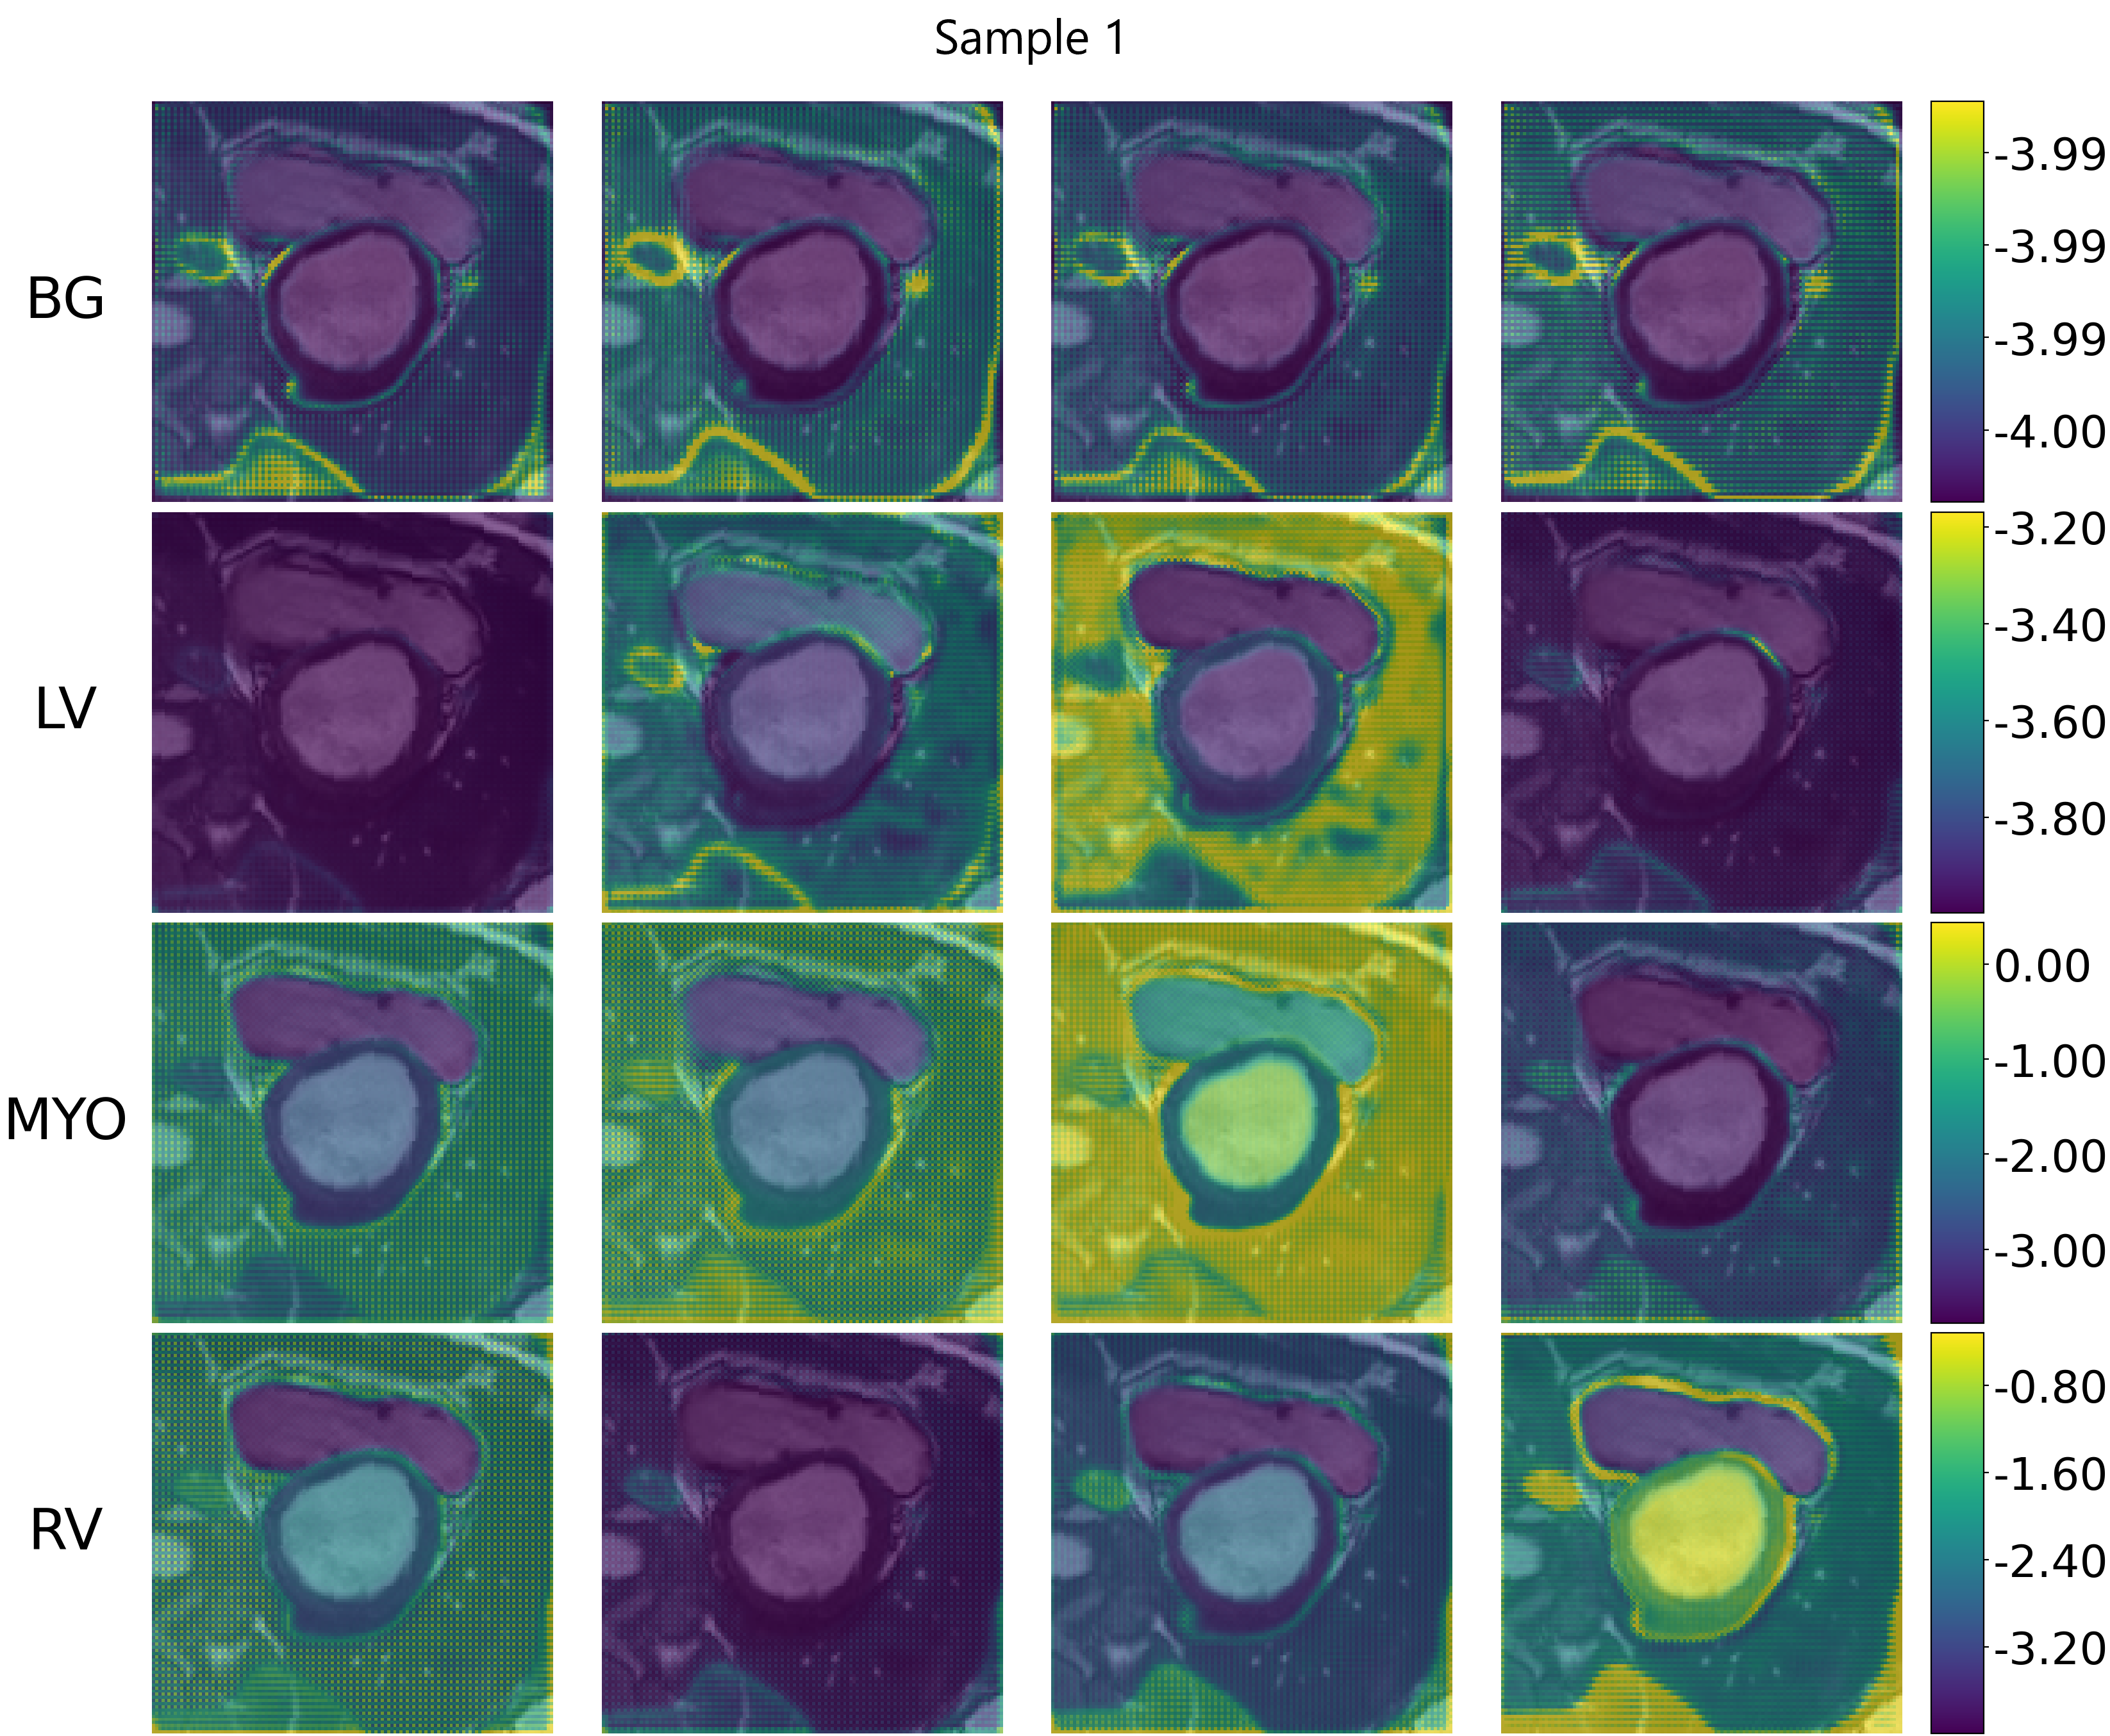
\includegraphics[width=0.48\linewidth]{Image/sigma1.png}
  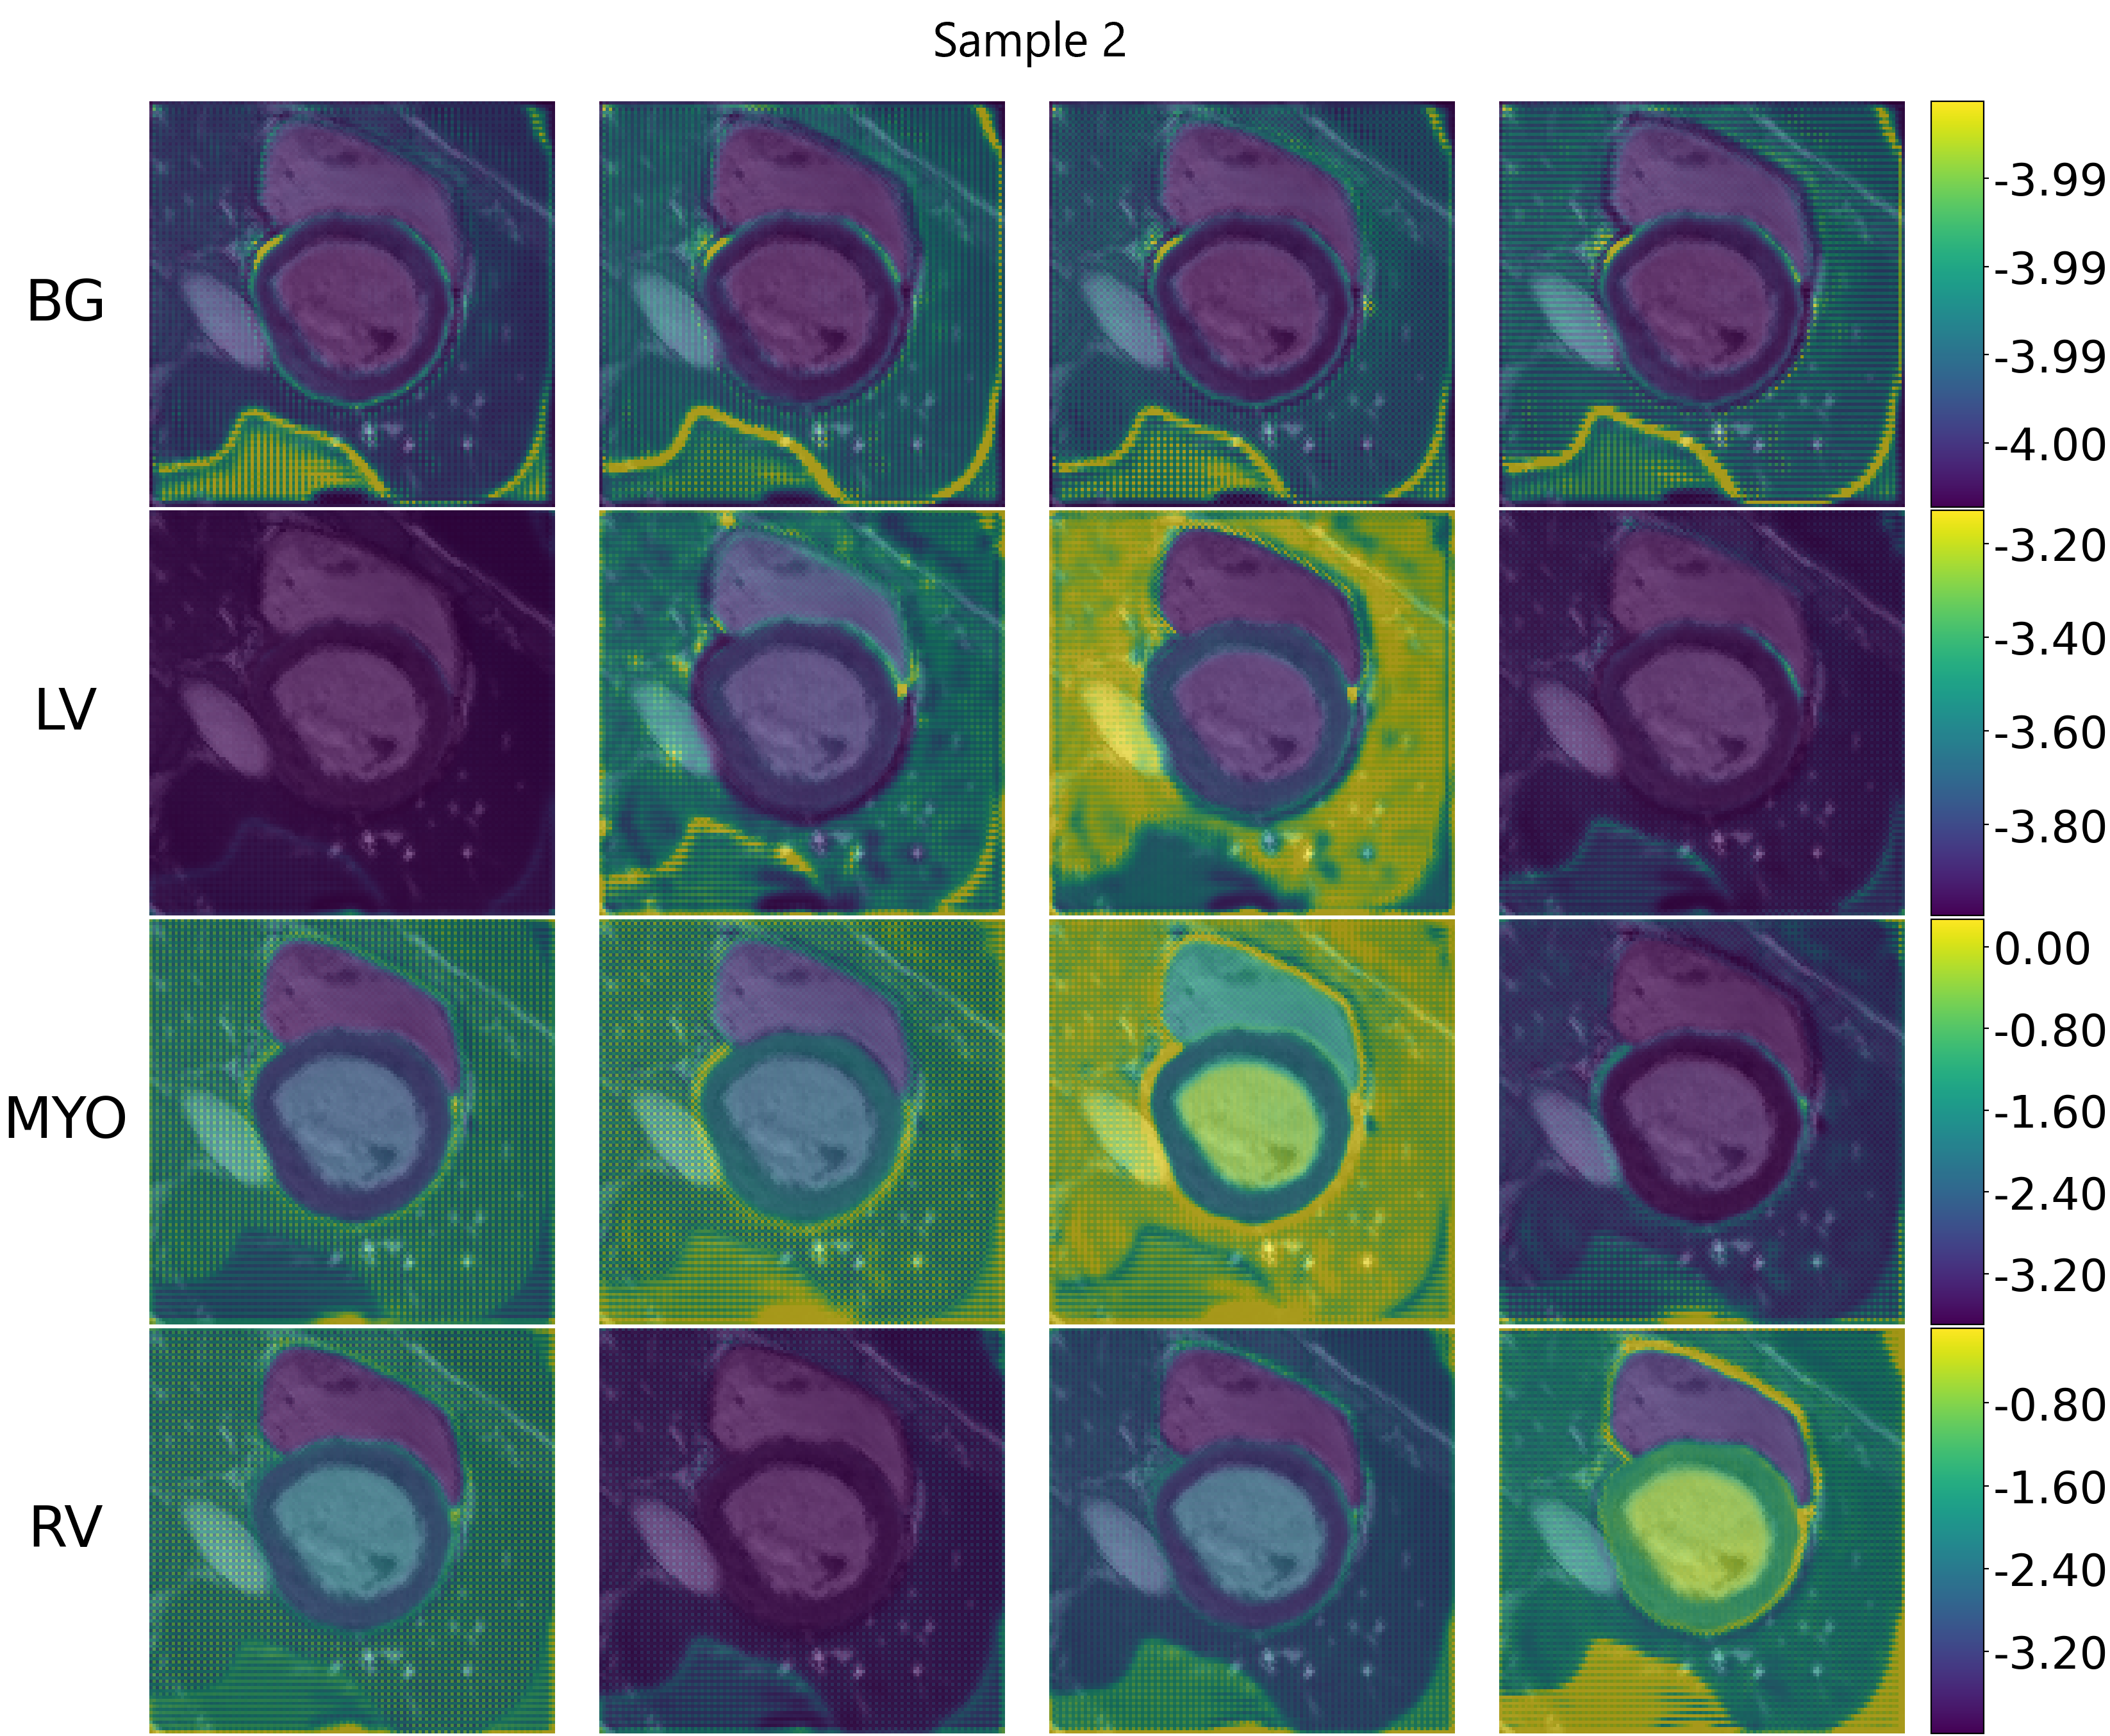
\includegraphics[width=0.48\linewidth]{Image/sigma2.png}
  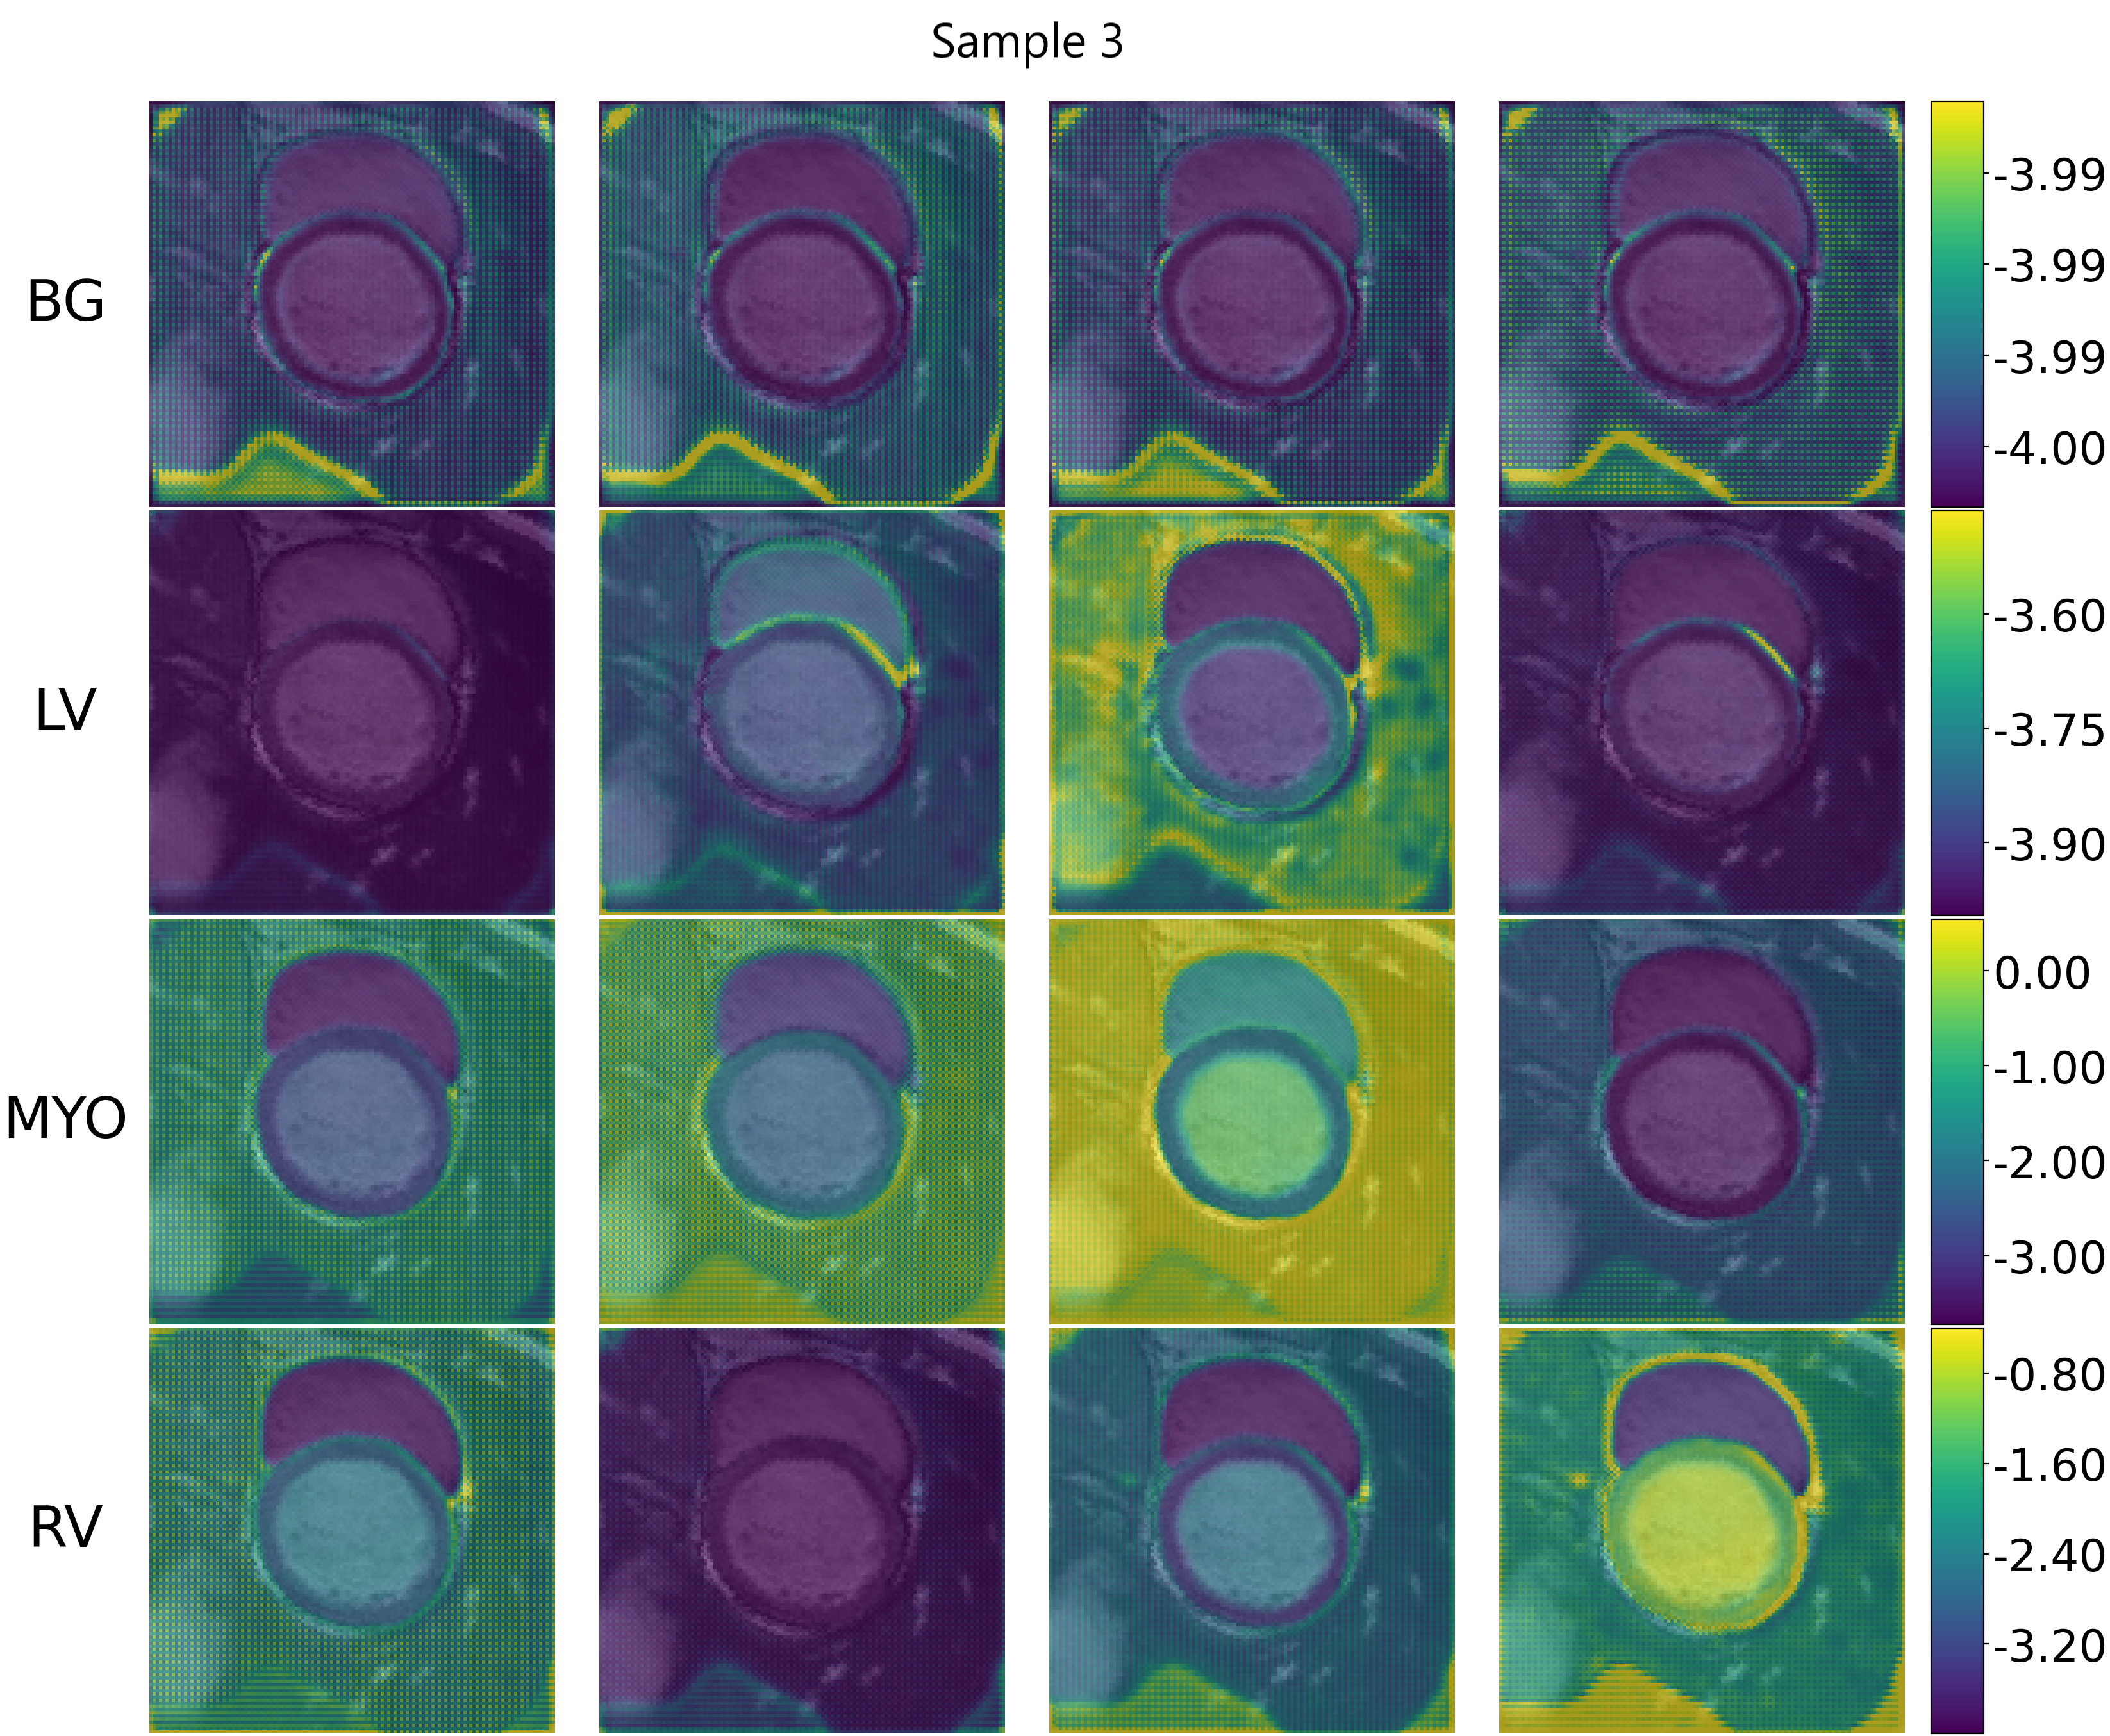
\includegraphics[width=0.48\linewidth]
  {Image/sigma3.png}
  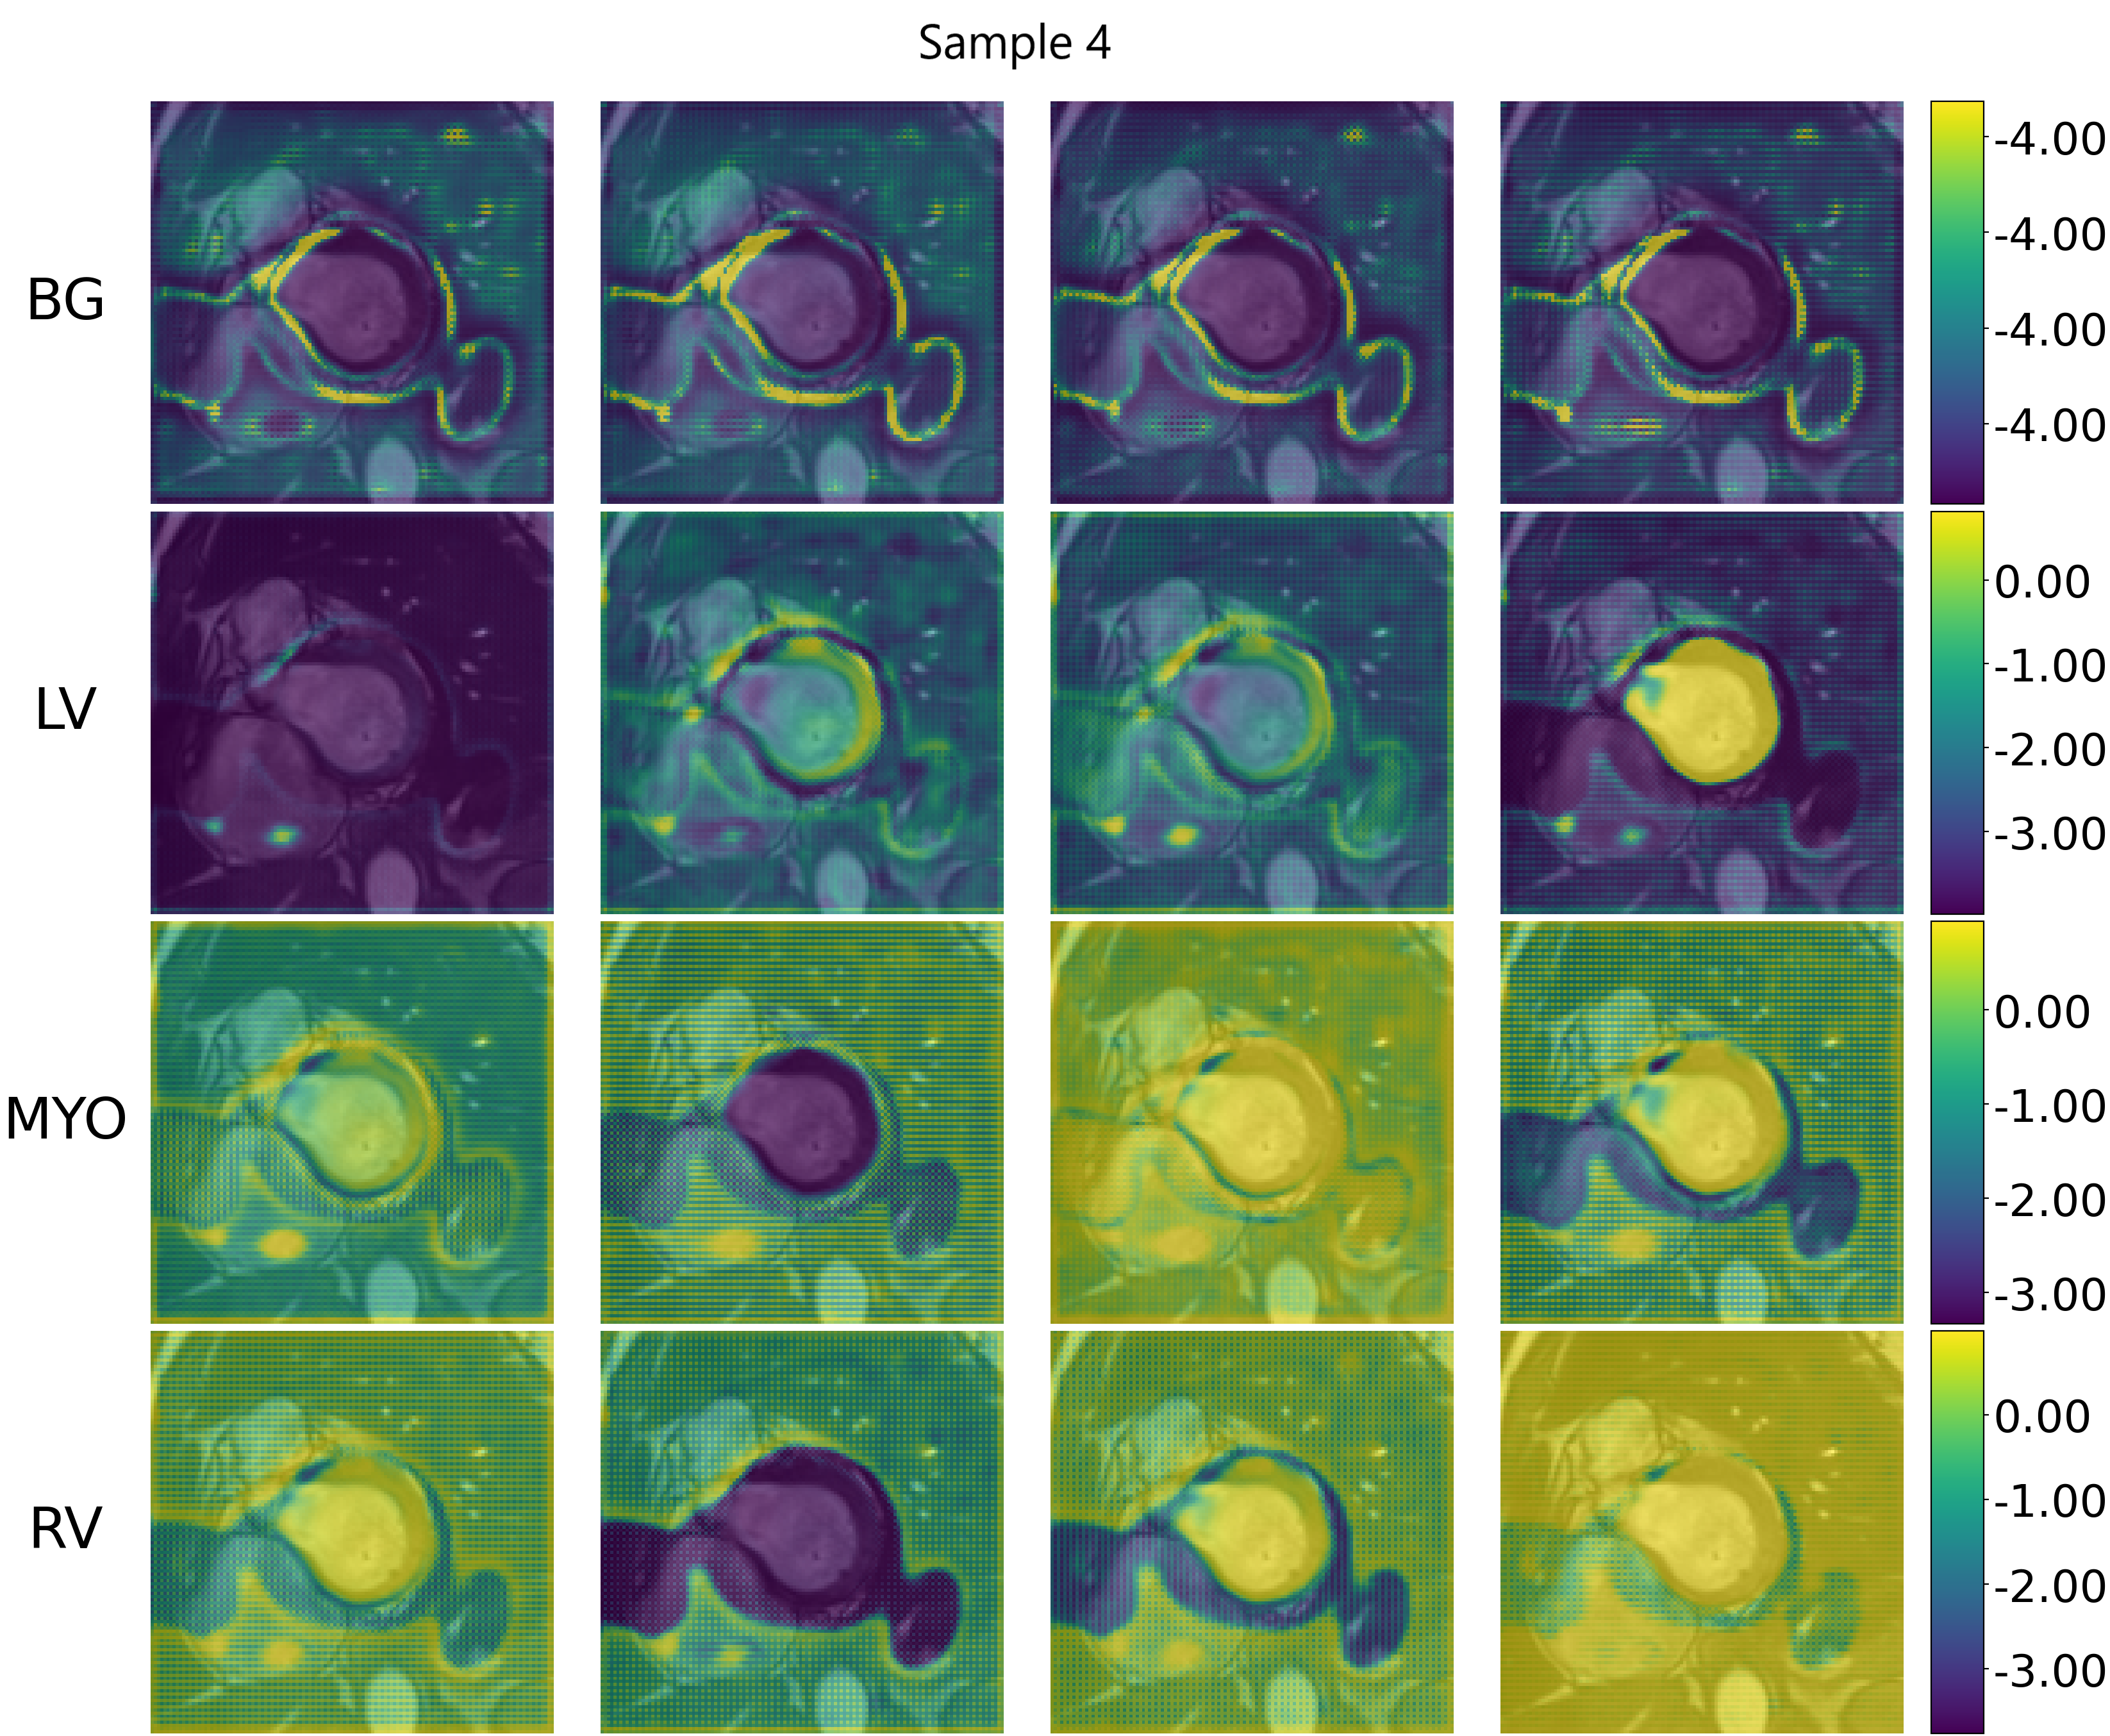
\includegraphics[width=0.48\linewidth]
  {Image/sigma4.png}
  \caption{Visualization of the log-variance for four samples. For each sample, the rows from top to bottom correspond to the four classes, while the columns from left to right correspond to the four feature dimensions.}
  \label{fig:Gaussian_var}
\end{figure}



The second term regularizes the posterior and prior of soft assignment
\begin{equation}
\label{loss2}
\begin{split}
  \mathcal{L}_2  &= \mathbb{E}_{q(\Omega\mid X)}\operatorname{KL}\big(q(Z\mid \Omega, X)\,\Vert\,p(Z\mid \Omega)\big)\\
  &= \int_{Z,\Omega} \log \frac{\prod_{i=1}^N\prod_{k=1}^K \pi_{ik}^{z_{ik}}}{\prod_{i=1}^N\prod_{k=1}^K \omega_{ik}^{z_{ik}}} q(Z\mid \Omega, X)q(\Omega\mid X)dZd\Omega\\
  &= \int_{Z,\Omega} \sum_{i=1}^N\sum_{k=1}^K z_{ik} \left(\log\pi_{ik}- \log \omega_{ik} \right)q(Z\mid \Omega, X)q(\Omega\mid X)dZd\Omega\\ 
  &= \int_{\Omega} \sum_{i=1}^N\sum_{k=1}^K \pi_{ik} \left(\log\pi_{ik}- \log \omega_{ik} \right)q(\Omega\mid X)d\Omega\\   
  &= \sum_{i=1}^N\sum_{k=1}^K \pi_{ik} \left(\log\pi_{ik}- \psi(d_{ik}) +\psi\left(\sum_{k=1}^K d_{ik}\right) \right),\\     
\end{split}
\end{equation}
where $\psi$ is the digamma function.
The discrete assignment latent variable $Z$ corresponds to the predictive class probability. This loss term $\mathcal{L}_2$ measures the discrepancy between the predicted class probability $q(Z\mid \Omega, X)$ and the prior class probability $p(Z\mid \Omega)$. 
Here, the prior class probability $p(Z\mid \Omega)$ guides the prediction results, which is obtained from the Gaussian mixture weights. 
%The larger mixture weights correspond to the higher prior probabilities for the associated classes. 


The third term regulates the predicted mixture weights using the anatomical prior.
\begin{equation}
\label{loss3}
\begin{split}
  \mathcal{L}_3  &= \operatorname{KL}\big(q(\Omega\mid X)\,\Vert\,p(\Omega\mid X)\big),\\
  &=\int_{\Omega} \log \frac{\prod_{i=1}^N\frac{1}{B(\boldsymbol{d}_i)}
\prod_{k=1}^K \omega_{ik}^{d_{ik} - 1}}{\prod_{i=1}^N\frac{1}{B(\boldsymbol{\hat{d}}_i)}
\prod_{k=1}^K \omega_{ik}^{\hat{d}_{ik} - 1}} q(\Omega\mid X) d\Omega\\
  &= \sum_{i=1}^N \log \frac{B(\boldsymbol{\hat{d}}_i)}{B(\boldsymbol{d}_i)}
+\sum_{i=1}^N\sum_{k=1}^K \left( d_{ik} - \hat{d}_{ik}\right) \left( \psi(d_{ik}) - \psi(\sum_{k=1}^K d_{ik}) \right).
\end{split}
\end{equation}


This loss term $\mathcal{L}_3$ serves as an important prior constraint, where cardiac anatomical structures are modeled as an anatomical structure prior to regularizing the predicted Gaussian mixture coefficients. Specifically, the feature distribution of each class is assumed to follow a class-specific Gaussian distribution derived from a dynamic cardiac anatomical prior. A higher mixture coefficient indicates a higher likelihood of assigning the corresponding class. In this way, the anatomical prior effectively encodes prior knowledge for category prediction. Therefore, this loss term effectively enforces the consistency between the predicted cardiac structures and the prior anatomical structure.


\subsection{Domain Generalization}
\label{sec:DG}
VGM-Seg can be interpreted as a prior-regularized variational generative model that performs pixel-wise density estimation in the feature space. Because VGM-Seg focuses on learning class-conditional feature distributions rather than domain-specific discriminative boundaries, it inherently has the ability to be robust under domain shifts.
%
This section will analyze the inherent domain generalization of VGM-Seg from the perspective of Invariant Mechanism Assumption (IMA)\cite{Peter2016Causal} that underlies domain generalization theory.

In IMA, class-conditional structures are assumed to be stable, while the marginal data distribution may vary across domains.
Formally, for data sampled from different domains $d \in \text{Domain}$,
\begin{equation}
p_d(\mathbf{x}, \mathbf{z}) = p_d(\mathbf{z} \mid \mathbf{x})\, p_d(\mathbf{x}),
\end{equation}
where $\mathbf{x}$ and $\mathbf{z}$ are data and the class label. IMA assumes that
\[
p_d(\mathbf{z} \mid \mathbf{x}) = p(\mathbf{z} \mid \mathbf{x}), \quad \forall d \in \text{Domain}.
\]
It implies that the predictive class $\mathbf{z}$ of data $\mathbf{x}$ is domain-invariant, whereas the variations arise mainly from changes in $p_d(\mathbf{x})$.


Traditional discriminative segmentation networks directly learn a discriminative mapping $f: \mathbf{x} \rightarrow \mathbf{z}$ on source-domain data, which implicitly approximates the posterior
\[
p(\mathbf{z} \mid \mathbf{x}) = \frac{p(\mathbf{x} \mid \mathbf{z})p(\mathbf{z})}{p(\mathbf{x})}.
\]
However, the class-conditional distributions $p(\mathbf{x} \mid \mathbf{z})$ and the class priors 
$p(\mathbf{z})$ are not explicitly constrained to remain invariant across domains.
When deployed in a new domain $d$, these underlying distributions may change, resulting in a different posterior $p_d(\mathbf{z} \mid \mathbf{x})$. Consequently, the discriminative mapping learned from the source domain may no longer remain optimal, leading to degraded performance. 

In contrast, our VGM-Seg models pixel-wise class-conditional density $p(\mathbf{x}_i \mid \mathbf{z}_i)$ in the feature space. Specifically, our VGM-Seg maximized the likelihood of features using class-conditional mixture Gaussian distributions, which encourages features of the same class to share a Gaussian distribution $\mathcal{N}(\boldsymbol{\mu}_{ik}, \boldsymbol{\Sigma}_{ik})$. 
%
The generative likelihood 
$
p(\mathbf{x}_i \mid \mathbf{z}_i=k) = \mathcal{N}(\mathbf{x}_i \mid \boldsymbol{\mu}_{ik}, \boldsymbol{\Sigma}_{ik})
$ 
captures the feature generation mechanism conditioned on anatomical class. 
Consequently, the segmentation decision $p(\mathbf{z}_i = k \mid \mathbf{x}_i) =
\frac{\omega_{ik} \, \mathcal{N}(\mathbf{x}_i \mid \boldsymbol{\mu}_{ik}, \boldsymbol{\sigma}^2_{ik})}
{\sum_{j=1}^{K} \omega_{ij} \, \mathcal{N}(\mathbf{x}_i \mid \boldsymbol{\mu}_{ij}, \boldsymbol{\sigma}^2_{ij})}$ arises from the learned class-conditional densities $p(\mathbf{x}_i \mid \mathbf{z}_i=k)$ and the Gaussian mixture weights $p(\mathbf{z}_i=k)=\omega_{ik}$. 
%Fortunately, $p(\mathbf{x}_i \mid \mathbf{z}_i)$ is domain invariant. 
Since the feature extractor captures anatomical structures instead of domain-specific appearance variations, the class-conditional feature distributions remain approximately invariant across domains. As a result, the likelihood 
$p(\mathbf{x}_i \mid \mathbf{z}_i)$ reflects primarily structure-induced feature similarity rather than domain discrepancy, making it largely domain-independent.
%
Moreover, $p(z_i=k)$ is related to the anatomical structure and is also domain invariant.
It implies that our VGM-Seg is naturally aligned with the invariant mechanism assumption and improves cross-domain generalization.



\subsection{Dirichlet Anatomical Prior}
\label{sec:prior}

In Eq.~\eqref{prior}, the dynamic prior $p(\Omega\mid X)$ describes the anatomical structure of the heart for the given image. To explicitly encode an anatomical prior, we first construct an empirical anatomical probability atlas from a small auxiliary labeled dataset $\mathcal{D}^l=\{(X^n,Y^n)\}_{n=1}^L$. Specifically, one label mask $Y^n$ is selected as the reference, and all labeled samples are registered to $Y^n$. For each pixel position, we compute the relative frequency of being annotated as each anatomical class. This yields a prior probability $\tilde{p}_{ik}$, the empirical probability of pixel $i$ belonging to class $k$. To avoid probabilities overly close to 0 or 1, we apply mild smoothing and clipping in practice.


Then, $\tilde{p}_{ik}$ is converted to Dirichlet concentration parameters:
\begin{equation}
  {d}^{(0)}_{ik} = \lambda\,\tilde{p}_{ik},
\end{equation}
where $\lambda$ controls the strength of the prior, $\lambda =10$ in this paper. 
${d}^{(0)}_{ik}$ models the concentration weight associated with the latent variable $z_{ik}$. A larger ${d}^{(0)}_{ik}$ implies a higher expected probability for the $i$-th pixel belonging to the $k$-th class. 
The summation $\sum_{k=1}^{K} {d}^{(0)}_{ik}$ represents the overall concentration of the Dirichlet distribution for a pixel: a higher value leads to a more confident distribution, whereas a lower value results in a more uncertain one.


Figure~\ref{fig:Dirichlet} illustrates the Dirichlet distributions of four samples drawn from the constructed anatomical prior. 
The four vertices of the tetrahedron correspond to the four classes 
$\boldsymbol{\pi}_1 = (1,0,0,0)$, $\boldsymbol{\pi}_2 = (0,1,0,0)$, $\boldsymbol{\pi}_3 = (0,0,1,0)$, and $\boldsymbol{\pi}_4 = (0,0,0,1)$. 
Randomly sampled points inside the tetrahedron describe the mixed class probability. A higher density of sampled points near a vertex indicates a higher probability of belonging to the corresponding class.
%
For example, Point 1 is located at the boundary between the background and RV, with Dirichlet samples distributed between $\boldsymbol{\pi}_1$ and $\boldsymbol{\pi}_4$.
In contrast, Point 3 lies inside the LV region, where Dirichlet samples concentrate near $\boldsymbol{\pi}_2$ and are distant from the other vertices, indicating a high probability of belonging to that class.
Details of constructing the Dirichlet prior are given in Algorithm~\ref{alg:dirichlet-prior}.



\begin{figure}[htpb]
  \centering
  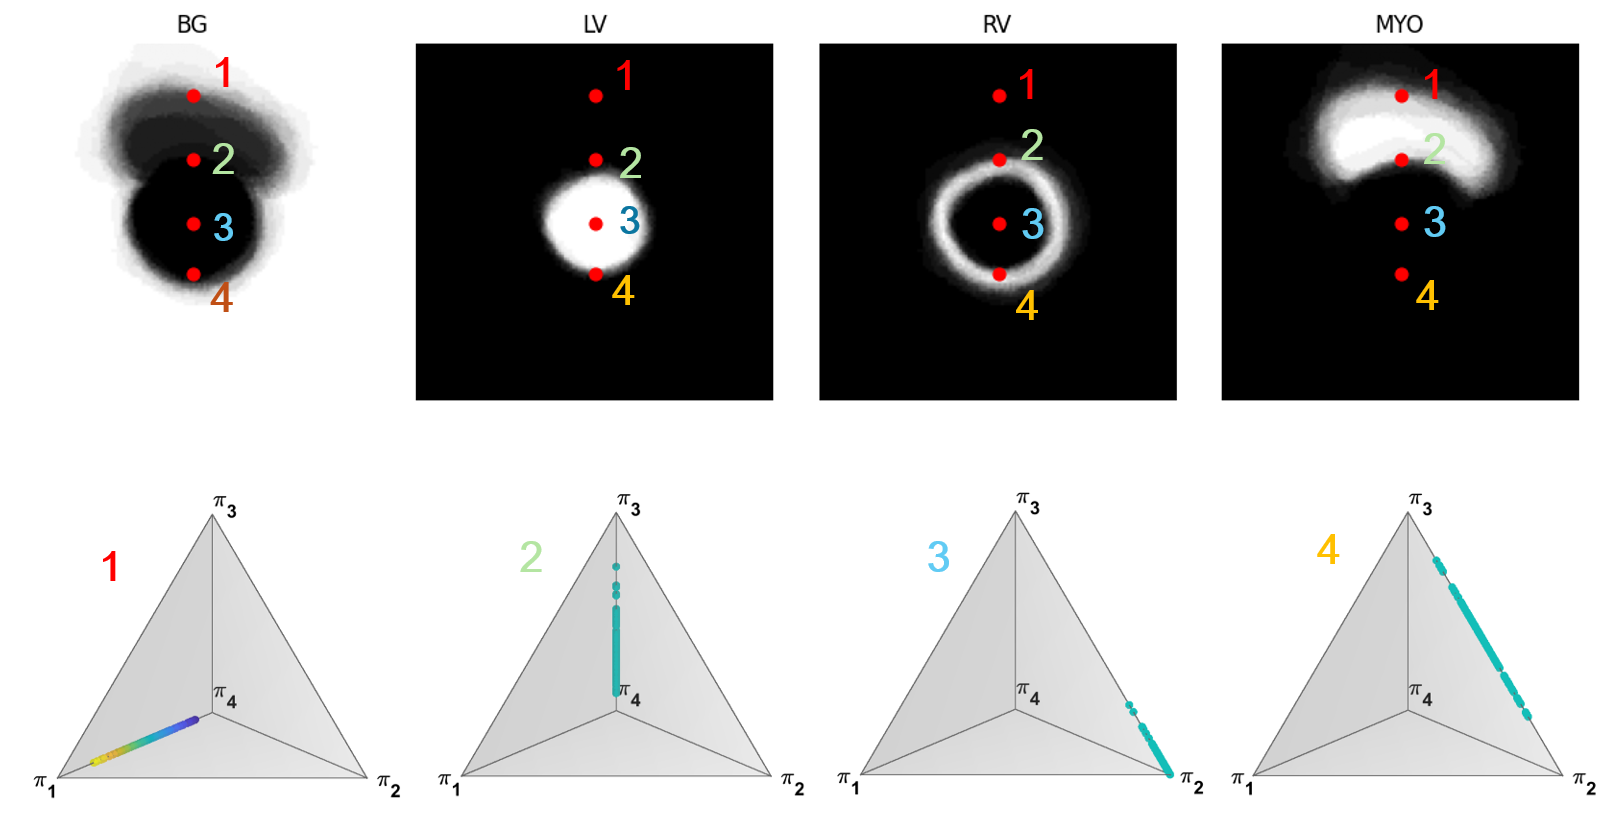
\includegraphics[width=1\linewidth]{Image/Dir.png}
  \caption{Visualization of the Dirichlet distributions for four samples drawn from the anatomical prior.}
  \label{fig:Dirichlet}
\end{figure}


\begin{algorithm}[t]
\caption{Constructing the Dirichlet anatomical prior}
\label{alg:dirichlet-prior}
\KwIn{The labeled dataset $\mathcal{D}^l=\{(X^n,Y^n)\}_{n=1}^L$, number of classes $K$, prior strength $\lambda>0$.}
\KwOut{Empirical probability $\tilde{p}$ and Dirichlet anatomical prior $d^{(0)}$.}
Select one label mask $Y^n$ as reference and register all other label masks to $Y^n$\;
\ForEach{pixel $i$}{
	\For{$k\leftarrow 1$ \KwTo $K$}{
		$\tilde{p}_{ik}\leftarrow \frac{1}{|\mathcal{D}^l|}\sum_{n} \mathbb{I}(Y^n_i=k)$ \tcp* {$\mathbb{I}(\cdot)$ is the indicator function} 
	}
}
Apply mild smoothing/clipping to $\tilde{p}$ to avoid values too close to 0 or 1\;
\Return $d^{(0)}\leftarrow \lambda\,\tilde{p}$\;
\end{algorithm}

For a given image $X$, its predicted Dirichlet distribution $q(\Omega \mid X)$ must be aligned with the Dirichlet prior $p(\Omega)$ due to their scale and translation differences.
We trained a registration module $f_{\text{reg}}$ to predict rigid transformation $\mathcal{T}_{\phi}$ with scale and translation parameters $\phi=(s,t_x,t_y)$. 
%
The registration network adopts ResNet-18 as the backbone. The final fully connected layer outputs parameters $\phi$. 
Pairs of training images are input to the network, which are generated by transforming the Dirichlet anatomical prior using random transformation parameters $\phi$. 
Mean Squared Error (MSE) is used as the registration loss $\mathcal{L}_{\text{reg}}$ to measure the discrepancy between the predicted transformation parameters $\hat{\phi}$ and the ground-truth $\phi$:
\[
\mathcal{L}_{\text{reg}} = \|\hat{\phi} - {\phi} \|_2^2.
\]


%The registration network is optimized using the Adam optimizer with an initial learning rate of $0.001$ for $100$ epochs. The registration performance is evaluated on the validation set after each epoch, and the model checkpoint with the lowest validation loss is retained.
%
When the registration network is trained, ${d}^{(0)}$ and the predicted ${d}$ are input to $f_{\text{reg}}$ to obtain $\mathcal{T}_{\phi}$. 
Then $\mathcal{T}_{\phi}$ maps the Dirichlet anatomical prior ${d}^{(0)}$ to a sample-specific prior of the given image $X$, denoted as the dynamic Dirichlet prior:
\begin{equation}
  \hat{d}_{ik} = \mathcal{T}_{\phi}\bigl({d}^{(0)}_{ik}\bigr).
\end{equation}

It should be noted that the dynamic Dirichlet prior $\hat{d}$ in our VGM-Seg model varies for each image $X$ during training, rather than being fixed.
This dynamic characteristic arises because the predicted mixture weights are continuously updated during training. After alignment, the dynamic Dirichlet prior evolves during training. 
Figure~\ref{fig:prior} illustrates the dynamic Dirichlet prior evolution throughout the training process. As training progresses and the prediction accuracy improves, the accuracy of the dynamic Dirichlet prior is gradually improved. Consequently, the dynamic Dirichlet prior is input-adaptive and sample-specific, providing tailored anatomical guidance for each image. 

\begin{figure}[htpb]
  \centering
  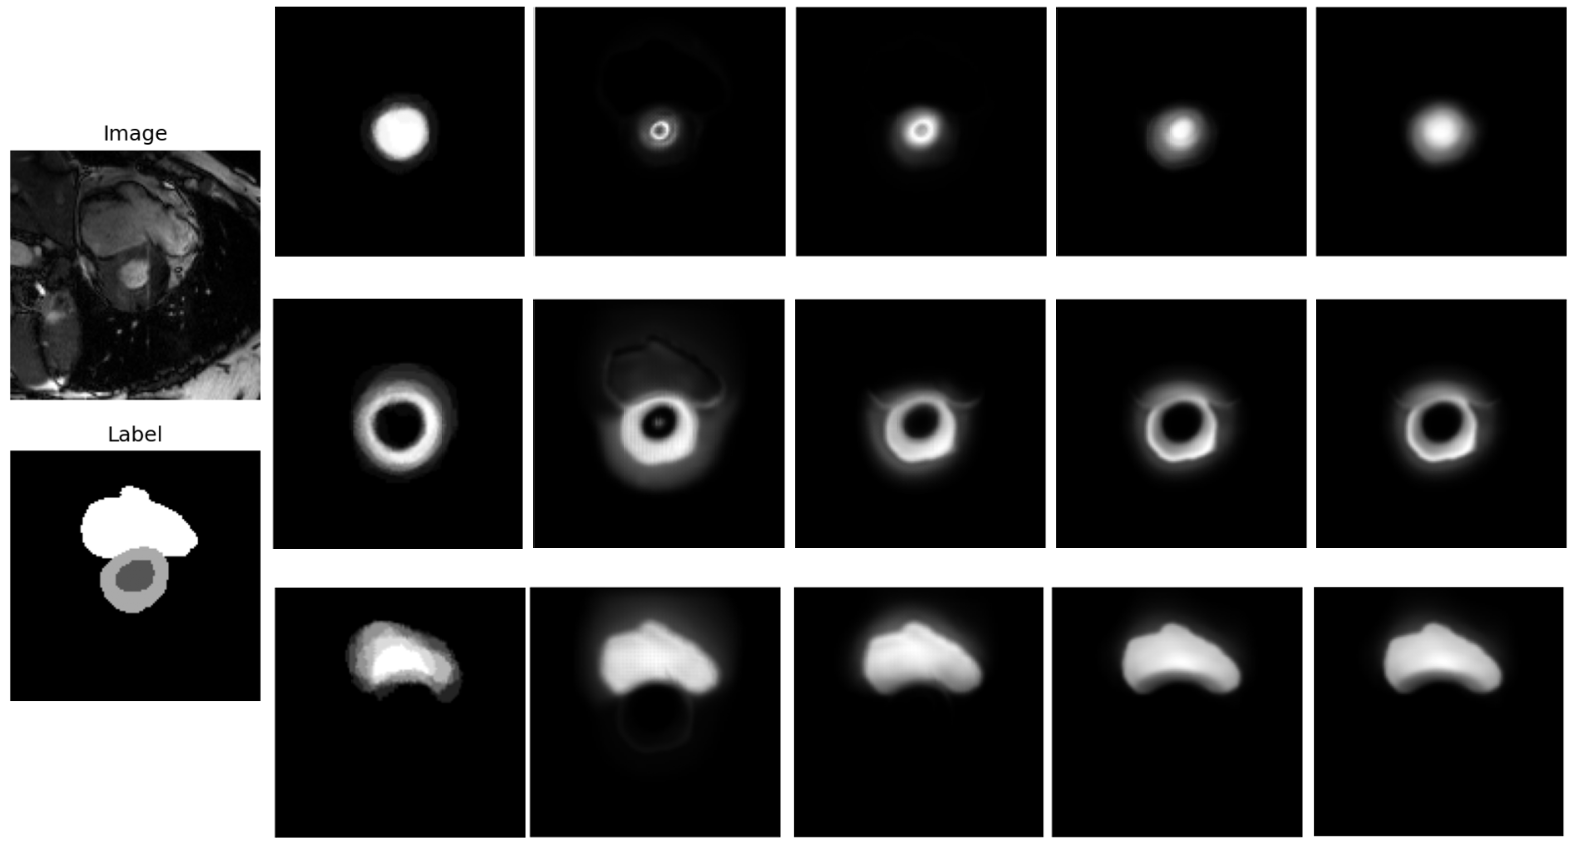
\includegraphics[width=0.8\linewidth]{Image/prior.png}
  \caption{Evolution of the dynamic prior during the training process. The leftmost shows the input image and its ground-truth label (for visualization only). The second column shows the Dirichlet anatomical prior $d^{(0)}$ of LV (top), MYO (middle), and RV (bottom). From left to right: evolution of the dynamic prior from early to late training stages.}
  \label{fig:prior}
\end{figure}




\subsection{Network Architecture and Training}

\subsubsection{Network Architecture}

\begin{figure}[t]
  \centering
  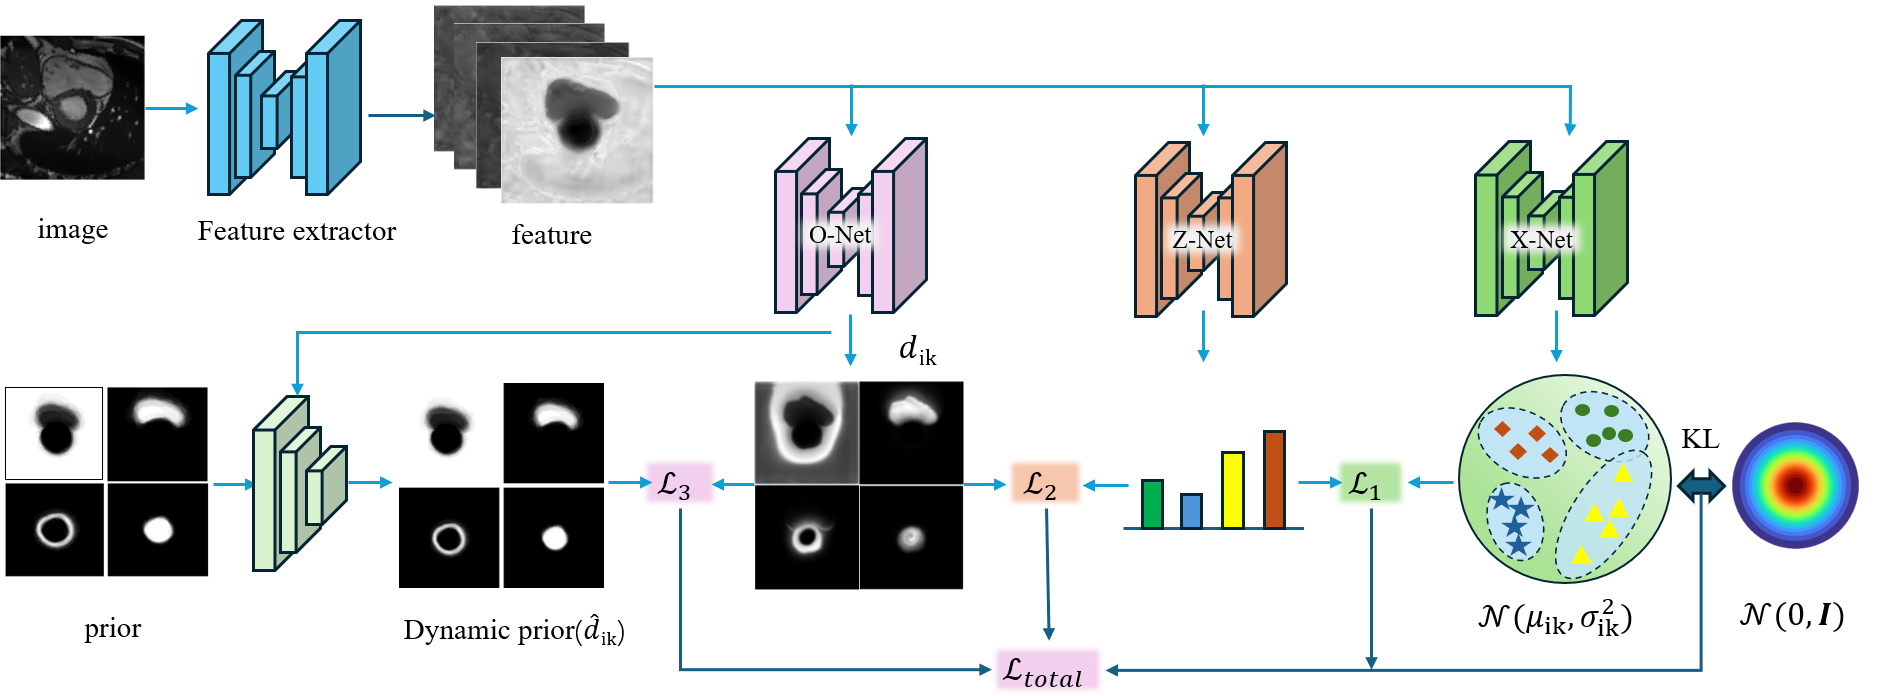
\includegraphics[width=\linewidth]{Image/framework.png}
  \caption{Overview of the proposed VGM-Seg framework. The sub-network \texttt{O-net} predicts the concentration parameter ${d}_{ik}$ of $q(\Omega \mid X)$, and further aligns to the Dirichlet prior to obtain the dynamic prior $p(\Omega \mid X)$.  \texttt{Z-net} predicts the distribution parameter of $q(Z \mid \Omega, X)$, and \texttt{X-net} predicts the mixture Gaussian distribution parameters $(\mu_{ik},\sigma^2_{ik})$. }
  \label{fig:framework}
\end{figure}

We combine deep learning with our variational GMM,  illustrated in Figure~\ref{fig:framework}. 
The features of the input image are extracted by a pre-trained feature extractor $\mathbf{E}$ and input into three sub-networks, \texttt{X-net}, \texttt{O-net}, and \texttt{Z-net}.
%
%
These sub-networks jointly parameterize the variational posteriors of the GMM.
\texttt{X-net} predicts the mixture Gaussian distribution parameters $(\boldsymbol{\mu_{ik}},\boldsymbol{\sigma}^2_{ik})$; 
\texttt{O-net} predicts the concentration parameter ${d}_{ik}$ of the Dirichlet distribution regularized by the aligned dynamic prior.
Consequently, the mixture weight $\omega_{ik}$ comes from the Dirichlet distribution 
$
\omega_{ik}\sim \mathrm{Dir}({d}_{ik}).
$
Given $\omega_{ik}$, the latent assignment variable $\mathbf{z}_{i}$ is predicted by \texttt{Z-net}:
\begin{equation}
\label{softassign}
q(\mathbf{z}_i = k \mid \Omega, X) = \boldsymbol{\pi}_{ik}.
\end{equation}
The predictive result is obtained by selecting the class with the maximum probability for each pixel:
\[
\hat{y}_i = \arg\max_{k \in \{1,\dots,K\}} \boldsymbol{\pi}_{ik}.
\]


%
We employ the U-Net architecture as the backbone of \texttt{X-net}, \texttt{Z-net}, \texttt{O-net}, and the feature extractor $\mathbf{E}$. 
It is worth noting that we adopt a basic U-Net architecture in this work. In practice, our framework is compatible with any segmentation network.
The \texttt{O-net} is pre-trained using the limited label dataset $\mathcal{D}^l$ to predict the concentration ${d}_{ik}$, where ${d}_{ik}$ is normalized as the probability $p_{ik}$ to compute a combination of Dice and Cross-Entropy loss.
\[
p_{ik} = \frac{{d}_{ik}}{\sum_{k} {d}_{ik}}.
\]

\texttt{X-net} is updated by maximizing the likelihood $\log p(X\mid Z,\Omega)$, and \texttt{Z-net} is updated by minimizing $\mathcal{L}_1$ and $\mathcal{L}_2$ to predict soft assignment $\boldsymbol{\pi}_{ik}$.
Furthermore, \texttt{O-net} is optimized by loss $\mathcal{L}_2$ and $\mathcal{L}_3$ to update the Dirichlet posterior over $d_{ik}$.
%Details of the pretraining \texttt{O-net} and the feature extractor $\mathbf{E}$ are presented in Section~\ref{sec:Onet}.

%During the forward pass, the feature maps extracted by $\mathbf{E}$ are input to three networks. \texttt{X-net} to predict the Gaussian mixture $\mathcal{N}(\mu_{ik},\sigma^2_{ik})$, and their corresponding weights $\pi_{ik}$ are predicted by \texttt{O-net}. Based on the weights $\pi_{ik}$, \texttt{Z-net} predicts the category for the $i$ pixel.


Three losses $\mathcal{L}_1, \mathcal{L}_2, \mathcal{L}_3$ contribute to the final loss as

\begin{equation}
\label{loss_total}
\mathcal{L}_{\text{total}}
= \mathcal{L}_1 + \lambda_1\,\mathcal{L}_2 + \lambda(e)\,\mathcal{L}_3
+ \lambda_2\,\sum_{i=1}^N\sum_{k=1}^K
\operatorname{KL}\Big(\mathcal{N}\big(\boldsymbol{\mu}_{ik}, \mathrm{diag}(\boldsymbol{\sigma}^2_{ik})\big)\,\Vert\,\mathcal{N}(\mathbf{0}, \mathbf{I})\Big).
\end{equation}

\begin{equation}
\operatorname{KL}\Big(\mathcal{N}\big(\boldsymbol{\mu}, \mathrm{diag}(\boldsymbol{\sigma}^2)\big)\,\Vert\,\mathcal{N}(\mathbf{0}, \mathbf{I})\Big)
= \frac{1}{2}\sum_{c=1}^{d}\left(-\log \sigma^2_{c} + \sigma^2_{c} + \mu^2_{c} - 1\right).
\end{equation}
where $\lambda_1$ and $\lambda_2$ are fixed coefficients, $\lambda(e)$ follows a cosine decay schedule over epochs $e$. The final term is the KL divergence between the predicted Gaussian and the standard Normal to prevent overfitting of Gaussian parameters.

\begin{equation}
    \lambda(e) = w_T+(w_0-w_T)\frac{1+cos(\pi e/T)}{2},
\end{equation}
where $w_0$ and $w_T$ are the initial and final coefficients, $T$ is the iteration number, $e$ is the current epoch.
Details of training VGM-Seg are provided in Algorithm~\ref{alg:vgmseg-train}.




% \subsubsection{Pretraining \texttt{O-net} and Feature Extractor}
% \label{sec:Onet}
% %$\texttt{O-net}$ has the architecture of a U-Net and is pretrained using limited labeled data, identical to those used for the prior distribution construction. 

% The pretraining of \texttt{O-net} and the feature extractor $\mathbf{E}$ is similar to training a segmentation network using a combination of Dice and Cross-Entropy loss to produce the predicted probability $p_{ik}$ of the $k$-th class for the pixel $i$.
% For \texttt{O-net}, $p_{ik}$ is the normalized concentration parameter ${d}_{ik}$.
% \[
% p_{ik} = \frac{{d}_{ik}}{\sum_{k} {d}_{ik}}.
% \]

% % The feature extractor is implemented as a U-Net architecture commonly used for image segmentation. 
% % Although trained with a limited amount of annotated data, the network's decoder learns high-level semantic representations, and we utilize the features from its final layer as the extracted features. 
% % These features capture the essential structural and anatomical information of the images while suppressing low-level texture details, reducing the modeling burden for the Gaussian mixture model.
% % It is important to emphasize that the feature extractor does not require high segmentation accuracy; it only needs to suppress low-level details while preserving high-level semantic information. Therefore, even a small amount of labeled data is sufficient for effective feature extraction.



\begin{algorithm}[t]
\caption{Training of VGM-Seg}
\label{alg:vgmseg-train}
\KwIn{Unlabeled dataset $\mathcal{D}^u=\{I^u\}$, Dirichlet anatomical prior $d^{(0)}$, number of classes $K$, hyperparameters $\lambda_1, \lambda_2, w_0, w_T$, and total iteration number $T$. 
Pre-trained networks: feature extractor $\mathbf{E}$, registration network $f_{\mathrm{reg}}$, and \texttt{O-net}.\\
}
\KwOut{Trained \texttt{O-net}, \texttt{Z-net} and \texttt{X-net}.}
Initialize \texttt{Z-net} and \texttt{X-net}\;
%Freeze $f_{\mathrm{enc}}$, $f_{\mathrm{reg}}$, and $f_{\mathrm{align}}$\;
\For{$e\leftarrow 1$ \KwTo $T$}{
	\ForEach{ $I^u$}{
		$\mathbf{x}\leftarrow \mathbf{E}(I^u)$ \tcp*{pixel-wise feature map}
		$\boldsymbol{\pi}\leftarrow \mathrm{Softmax}\bigl(\texttt{Z-net}(\mathbf{x})\bigr)$ \tcp*{$q(Z\mid \Omega, X)$}
		$ \tilde{d}\leftarrow \mathrm{Softplus}\bigl(\texttt{O-net}(\mathbf{x})\bigr)$ \tcp*{$q(\Omega\mid X)$}

		$\mathcal{T}_{\phi} \leftarrow f_{\mathrm{reg}}\bigl(d^{(0)},\ \tilde{d}\bigr)$\;
    $ \hat{d} \leftarrow \mathcal{T}_{\phi}(d^{(0)})$ \tcp*{aligned dynamic Dirichlet prior}
		$(\boldsymbol{\mu},\boldsymbol{\sigma}^2)\leftarrow \texttt{X-net}(\mathbf{x})$ \tcp*{$p(X\mid \Omega, Z)$}
        $\lambda(e) = w_T+(w_0-w_T)\frac{1+\cos(\pi e/T)}{2}$\;
        Compute loss $\mathcal{L}$ using Eq.~\ref{loss_total}\; 
		Update weights of \texttt{O-net}, \texttt{Z-net} and \texttt{X-net} by backpropagation\;
	}
}
\Return{ \texttt{O-net}, \texttt{Z-net} and \texttt{X-net}}\;
\end{algorithm}

\subsection{Segmentation Uncertainty}

Beyond unsupervised segmentation, another key advantage of our VGM-Seg is its ability to quantify uncertainty in the segmentation results through a variational Gaussian mixture model.
Since segmentation labels arise from posterior inference under a class-conditional Gaussian mixture distribution, the segmentation uncertainty can be naturally quantified by posterior entropy rather than classifier ambiguity.  
That is, the segmentation uncertainty provided by our VGM-Seg is derived from the feature-space likelihood overlap, which provides a principled measure of intrinsic data ambiguity instead of uncertainty caused by limited model capacity.



The latent variable
$z_{ik}$ indicates the assignment of the components of the mixture, which is inferred by $q(\mathbf{z}_i = k \mid \Omega, X)$ in Eq.~\eqref{softassign}.
%
This posterior provides an explicit predictive probability and segmentation uncertainty of pixel-wise segmentation:
\begin{equation}
\mathcal{U}_{i}=- \sum_{k=1}^K \boldsymbol{\pi}_{ik} \log \boldsymbol{\pi}_{ik}.
\end{equation}
$\mathcal{U}_{i}$ with low value indicates confidence in the prediction results.



Furthermore, in cross-domain scenarios, segmentation uncertainty mainly arises from distributional discrepancies between domains. Within the VGM-Seg framework, such cross-domain uncertainty is naturally reflected in the posterior distributions of the latent variables. Experimental results show that segmentation predictions in previously unseen domains exhibit lower confidence compared to those produced by domain-adaptation (DA) methods.


%



\section{Experiments and Results}
\subsection{Datasets and Implementation Details}
We evaluated VGM-Seg on four public cardiac MRI datasets: ACDC~\cite{Bernard2018Deep}, M\&Ms~\cite{Campello2021Multi}, SCD~\cite{radau2009evaluation} and York~\cite{andreopoulos2008efficient}.

\begin{itemize}
  \item \textbf{ACDC}: A multi-center cine MRI dataset comprises 150 patients with different clinical conditions. Each patient consists of 28–40 short-axis cine MRI during a cardiac cycle. Each image is labeled with pixel-wise annotations for LV, RV, and MYO. 
  We used part of the ACDC dataset to build the anatomical prior.
  \item \textbf{M\&Ms}: A multi-vendor dataset with notable domain shifts across four vendors and acquisition protocols, suitable for cross-domain generalization evaluation. 
It contains a total of 375 patient scans.
Annotations of the LV, RV, and MYO in the end-diastole (ED) and end-systole (ES) phases are provided.
  
 \item \textbf{SCD}: Sunnybrook Cardiac Dataset, originally used in the LV Segmentation Challenge, containing 45 subjects with high-quality LV annotations.
 LV annotations are available for ED and ES. Specifically, the inner contours of the LV are annotated in both the ED and the ES, while the outer contours are annotated in the ES.
  
  \item \textbf{YORK}: A dataset focusing on LV and MYO segmentation. It consists of short-axis MRI scans of 33 children, and experienced clinicians manually annotated the LV to provide ground-truth labels.
\end{itemize}

In the unsupervised setting, we only used 352 labeled data collected from 25 patients from the ACDC dataset to construct the Dirichlet anatomical prior. We then trained and evaluated VGM-Seg on all target datasets without any other labels. We report Dice scores, Jaccard, HD95, and ASD averaged over predictive results.


All experiments were implemented with Python~3.11 and PyTorch~2.x on a single NVIDIA GeForce RTX 3080 GPU. We use a batch size of 16 and set the initial learning rate to $5\times 10^{-4}$. We use the Adam optimizer~\cite{adam} with a \texttt{ReduceLROnPlateau} scheduler that reduces the learning rate according to the validation loss. All input images are cropped to $128\times 128$, and the hyperparameters are set as $\lambda_1=10$, $\lambda_2=0.001$, and $\lambda(e)$ decays from 1.0 to 0.001 with a cosine schedule.



\subsection{Hyperparameters}

\begin{figure}[htpb]
  \centering
  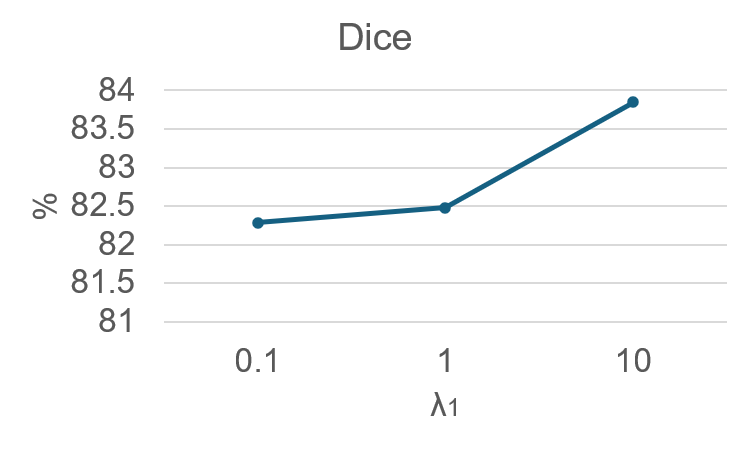
\includegraphics[width=0.4\linewidth]{Image/lambda1.png}
  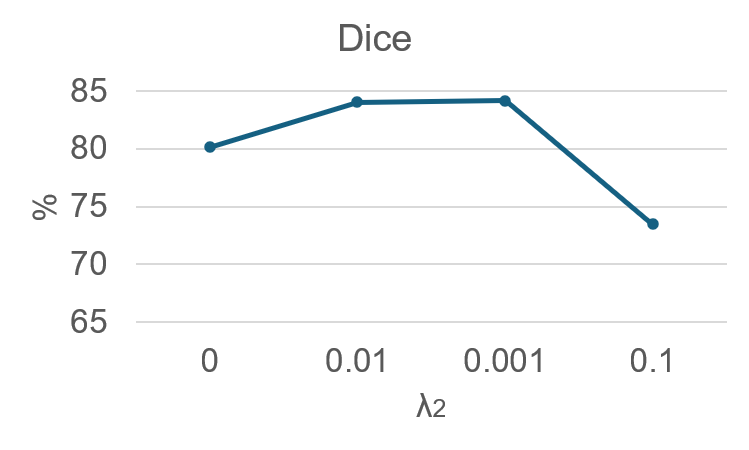
\includegraphics[width=0.4\linewidth]{Image/lambda2.png}
  \caption{Sensitivity of model performance with respect to the two hyperparameters $\lambda_1$ and $\lambda_2$.}
  \label{fig:hyperparameter}
\end{figure}

Figure~\ref{fig:hyperparameter} shows the influence of the two hyperparameters $\lambda_1$ and $\lambda_2$ on the performance of VGM-Seg. %$\lambda_1$ controls the contribution of the GMM reconstruction loss. As shown in Figure~\ref{fig:hyperparameter}, $\lambda_1$ should not be set too large, since a large $\lambda_1$ causes VGM-Seg to focus overly on GMM reconstruction while neglecting the classification. 
$\lambda_1$ regularizes the KL divergence between the latent variables predicted for classification and the dynamic prior, which corresponds to the predictive accuracy of the mixture weights. A larger $\lambda_1$ is beneficial to improve classification accuracy, because it directly influences classification results. 
%
$\lambda_2$ controls the contribution of the KL divergence term to the overall loss. 
An excessively large $\lambda_2$, such as 0.1,  results in a significant degradation in segmentation accuracy, 
while within a relatively small range, the performance of the model is not sensitive to the value of $\lambda_2$.
We set $\lambda_1 = 10$ and $\lambda_2 = 0.001$ in our experiments.


\subsection{Results}

This section compares the segmentation performance of VGM-Seg with different models on various datasets. The models compared include GMM-based, semi-supervised, and unsupervised domain adaptation (DA) methods. 
%The DA methods used labeled source domain data and unlabeled target domain data.

\subsubsection{Comparison with GMM-based Methods}

In this experiment, we compare VGM-Seg with traditional GMM~\cite{zhang2002segmentation} and DeepSVG~\cite{deepGMM}, where GMM is the traditional Gaussian Mixture Model with iterative expectation maximization, and DeepSVG estimated parameters of a GMM using a CNN by minimizing the
NLL function of the GMM.
%
Since GMM and DeepSVG exhibit limited performance when modeling Gaussian mixtures directly in the image intensity space, we use the extracted image features as input for both GMM and DeepSVG to construct the Gaussian mixtures in this experiment. This setting enables a fair comparison and better highlights the advantages of the proposed variational GMM framework.

% 表格1: GMM 数据集结果
\begin{table}[htbp]
  \centering
  \caption{Performance comparison with GMM-based methods on different datasets.}
%  \resizebox{\linewidth}{!}{%
  \begin{tabular}{l c c c c c}
    \toprule
    Datasets & Method &  Dice(\%)$\uparrow$ & Jaccard(\%)$\uparrow$ & HD95$\downarrow$ & ASD$\downarrow$ \\
    \midrule
    \multirow{3}{*}{ACDC} & GMM~\cite{zhang2002segmentation} &  36.78 & 27.92 &  41.49 & 18.23 \\
    & DeepSVG~\cite{deepGMM} &  30.86 & 22.58 & 46.62 & 22.62 \\
    & Ours & \textbf{87.71} & \textbf{78.54} & \textbf{2.36} & \textbf{0.69} \\
    \midrule
    \multirow{3}{*}{M\&Ms} & GMM~\cite{zhang2002segmentation} & 43.00 & 33.41 & 36.22 & 15.57 \\
    & DeepSVG~\cite{deepGMM} & 37.47 & 28.77 & 42.74 & 19.79 \\
    & Ours &  \textbf{83.85} & \textbf{71.41} & \textbf{2.50} & \textbf{0.76} \\
    \midrule
    \multirow{3}{*}{SCD} & GMM~\cite{zhang2002segmentation} &  15.29 & 10.46 & 47.45 & 24.82 \\
    & DeepSVG~\cite{deepGMM} &  44.51 & 30.84 & 31.05 & 14.79 \\
    & Ours & \textbf{90.91} & \textbf{83.76} & \textbf{4.56} & \textbf{1.14} \\
    \midrule
    \multirow{3}{*}{York} & GMM~\cite{zhang2002segmentation} &  23.96 & 15.43 & 41.57 & 20.91 \\
    & DeepSVG~\cite{deepGMM} &  23.70 & 14.97 & 35.43 & 15.56 \\
    & Ours & \textbf{84.15} & \textbf{74.25} & \textbf{2.28} & \textbf{0.78} \\
    \bottomrule
  \end{tabular}%
%  }
  \label{tab:GMM}
\end{table}


%表格内容需要重新做，重新分析
Table \ref{tab:GMM} lists the performance comparison in the ACDC, M\&Ms, SCD and York datasets. It can be observed that our VGM-Seg preserves stable segmentation performance across all four datasets and outperforms GMM and DeepSVG. This is mainly because they lack sufficient capacity to model complex anatomical structures in cardiac images using a mixture of multi-Gaussian representations. It indicates the advantages of anatomical priors and variational inference in our VGM-Seg. 


More importantly, note that the York dataset consists of pediatric cardiac images, where the heart objects are small and the underlying pathologies are complex, making segmentation particularly challenging and leading to a pronounced performance degradation for GMM and DeepSVG. 
In contrast, our proposed VGM-Seg maintains stable prediction performance in the York dataset and achieves a substantial improvement over both GMM and DeepSVG, demonstrating its robustness in challenging complex cardiac imaging scenarios.


%这个图要补充，然后分析
Figure~\ref{fig:tsneGMM} illustrates $\boldsymbol{\mu}$ and its t-SNE visualization of the mixture Gaussians estimated by GMM, DeepSVG, and our VGM-Seg, respectively. Compared with GMM and DeepSVG, which result in substantial inter-class overlap, VGM-Seg predicts the mean of the mixture Gaussian with significantly better inter-class separation. 
The Gaussian means $\boldsymbol{\mu}$ estimated by our VGM-Seg exhibit greater distinctiveness between classes within their corresponding categories (as reflected along the diagonal), which facilitates clearer separation between different classes.

\begin{figure}[t]
  \centering
  \includegraphics[width=0.8\linewidth]{Image/mu.png}  
  \caption{$\boldsymbol{\mu}$ and its t-SNE visualization estimated by GMM, DeepSVG, and VGM-Seg, respectively.}
  \label{fig:tsneGMM}
\end{figure}


%%%%%%%%%%%%%%%%%%%%%%%%%%%
\subsubsection{Comparison with Semi-supervised Models}

We compare VGM-Seg with recent semi-supervised learning (SSL) cardiac segmentation methods such as SS-Net\cite{SS-Net}, DC-Net\cite{DC-Net}, ABD\cite{ABD}, LSRL-Net\cite{liu2025lsrl}, beta-FFT\cite{beta-FFT}, and ALHVR\cite{ALHVR}. 
Table \ref{tab:segSemi} presents the performance comparison of VGM-Seg with other SSL models. For the M\&Ms dataset, SSL methods are trained with 5\% labeled data, whereas VGM-Seg achieves a mean Dice score of 83.85\% without using any labeled data, outperforming other SSL methods by an average of 4.4\% in Dice. 

% 表格1: MM 数据集结果
\begin{table}[htbp]
  \centering
  \caption{Performance comparison of different semi-supervised models on various datasets.}
  \resizebox{\linewidth}{!}{%
  \begin{tabular}{l c c c c c c}
    \toprule
    Type & Method & Label ratio & Dice(\%)$\uparrow$ & Jaccard(\%)$\uparrow$ & HD95$\downarrow$ & ASD$\downarrow$ \\
    \midrule
    \multirow{7}{*}{M\&Ms} & SS-Net\cite{SS-Net} & \multirow{7}{*}{5\%} & 72.58±21.42 & 63.68±21.61 & 7.26±8.54 & 2.86±3.93 \\
    & DC-Net\cite{DC-Net} & & 80.67±14.98 & 72.06±15.64 & 3.96±3.52 & 1.55±1.56 \\
    & ABD\cite{ABD} & & 80.35±20.54 & 72.22±20.41 & 3.47±3.45 & 1.34±1.84 \\
    & LSRL-Net\cite{liu2025lsrl} & & 82.06±23.75 & 70.22±22.24 & 2.56±9.47 & 0.70±5.79 \\
    & Beta-FFT\cite{beta-FFT} & & 82.70±17.86 & \textbf{74.84±18.46} & 3.73±5.74 & 1.51±2.15 \\
    & ALHVR\cite{ALHVR} & & 78.30±19.74 & 70.05±19.48 & \textbf{2.13±3.16} & \textbf{0.46±1.30} \\
    & Ours & - & \textbf{83.85±21.03} & 71.41±20.68 & 2.50±6.97 & 0.76±4.75 \\
    \hline
        \multirow{7}{*}{SCD} & SS-Net\cite{SS-Net} & \multirow{7}{*}{10\%} & 81.31±21.69 & 72.76±23.72 & 5.69±4.69 & 2.48±2.19 \\
    & DC-Net\cite{DC-Net} & & 87.64±14.49 & 80.37±18.59 & 3.96±3.46 & 1.80±1.73 \\
    & ABD\cite{ABD} & & 89.20±14.61 & 82.85±18.09 & 3.05±2.67 & 1.45±1.50 \\
    & LSRL-Net\cite{liu2025lsrl} & & 88.23±15.95 & 78.94±20.00 & 4.00±5.94 & 1.18±2.27 \\
    & Beta-FFT\cite{beta-FFT} & & 88.48±15.01 & 81.82±18.60 & 3.60±3.49 & 1.71±1.90 \\
    & ALHVR\cite{ALHVR} & & 87.16±15.78 & 79.97±19.77 & \textbf{2.00±3.21} & \textbf{0.58±1.20} \\
    & Ours & - & \textbf{90.91±10.40} & \textbf{83.76±14.18} & 4.56±4.97 & 1.14±1.42 \\
    \hline
        \multirow{7}{*}{York} & SS-Net\cite{SS-Net} & \multirow{7}{*}{10\%} &60.32±26.00 & 50.51±24.52 & 7.81±5.72 & 2.02±1.60 \\
    & DC-Net\cite{DC-Net} & & 70.25±25.26 & 60.13±24.44 & 5.69±4.87 & 1.81±1.29 \\
    & ABD\cite{ABD} & & 81.04±16.97 & 71.58±18.19 & 4.22±3.20 & 1.71±1.70 \\
    & LSRL-Net\cite{liu2025lsrl} & & 71.60±20.92 & 56.26±21.77 & 4.70±6.11 & 1.36±2.60 \\
    & Beta-FFT\cite{beta-FFT} & & 76.86±18.93 & 66.27±20.72 & 4.98±3.47 & 2.29±2.03 \\
    & ALHVR\cite{ALHVR} & & 79.00±16.95 & 68.54±18.99 & 2.67±3.04 & \textbf{0.54±1.07} \\
    & Ours & - & \textbf{84.15±17.76} & \textbf{74.25±18.77} & \textbf{2.28±4.58} & 0.78±1.83 \\
    \hline
        \multirow{7}{*}{ACDC} & SS-Net\cite{SS-Net} & \multirow{7}{*}{10\%} & 76.77±23.44 & 68.53±23.33 & 4.78±5.48 & 1.74±1.93 \\
    & DC-Net\cite{DC-Net} & & 79.23±20.16 & 71.21±20.54 & 5.32±8.24 & 2.18±4.20 \\
    & ABD\cite{ABD} & & 80.58±21.55 & 73.91±21.57 & 3.71±6.72 & 1.60±3.91 \\
    & LSRL-Net\cite{liu2025lsrl} & & 80.83±22.06 & 68.36±22.01 & 6.72±7.12 & 1.12±3.54 \\
    & Beta-FFT\cite{beta-FFT} & & 85.29±15.75 & \textbf{78.83±16.29} & 3.24±6.06 & 1.13±2.34 \\
    & ALHVR\cite{ALHVR} & & 80.19±22.02 & 71.89±22.49 & 2.51±6.70 & \textbf{0.66±2.33} \\
    & Ours & - & \textbf{87.71±20.31} & 78.54±20.46 & \textbf{2.36±7.16} & 0.69±4.61 \\
    \bottomrule
  \end{tabular}%
  }
  \label{tab:segSemi}
\end{table}


It should be noted that the M\&Ms dataset includes data acquired from four different vendors.
The 5\% labeled data are randomly sampled from four vendors, allowing the evaluation of the generalization of the model under mixed-domain conditions.
We further analyzed the prediction accuracy for each vendor by plotting boxplots of the Dice scores. As shown in Figure~\ref{MMboxplot}, it indicates that our VGM-Seg maintains robust performance under mixed-domain conditions.


\begin{figure}[htpb]
  \centering
  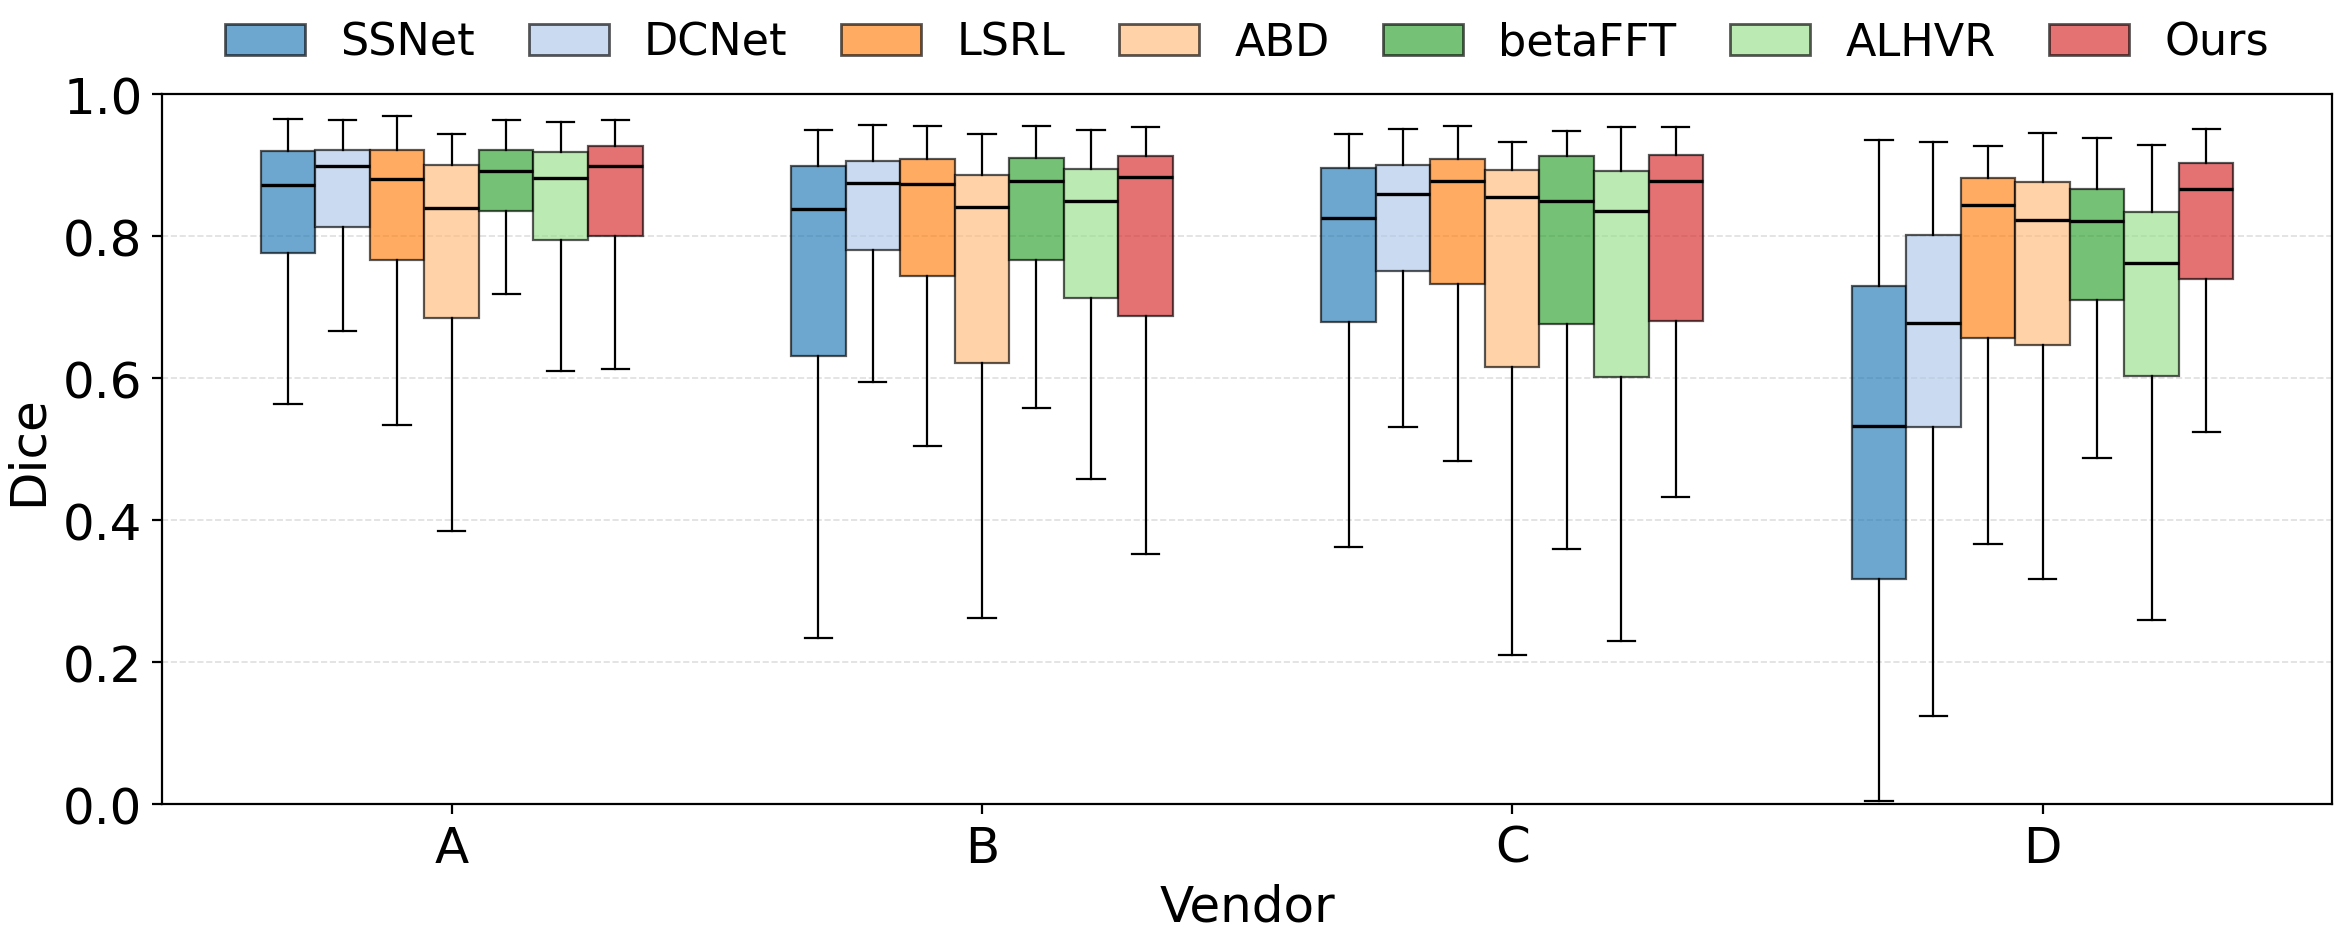
\includegraphics[width=0.8\linewidth]{Image/boxplotMM.png}
  \caption{Dice boxplot comparison between VGM-Seg and SSL methods on the M\&Ms dataset.}
  \label{MMboxplot}
\end{figure}


\begin{figure}[htpb]
  \centering
  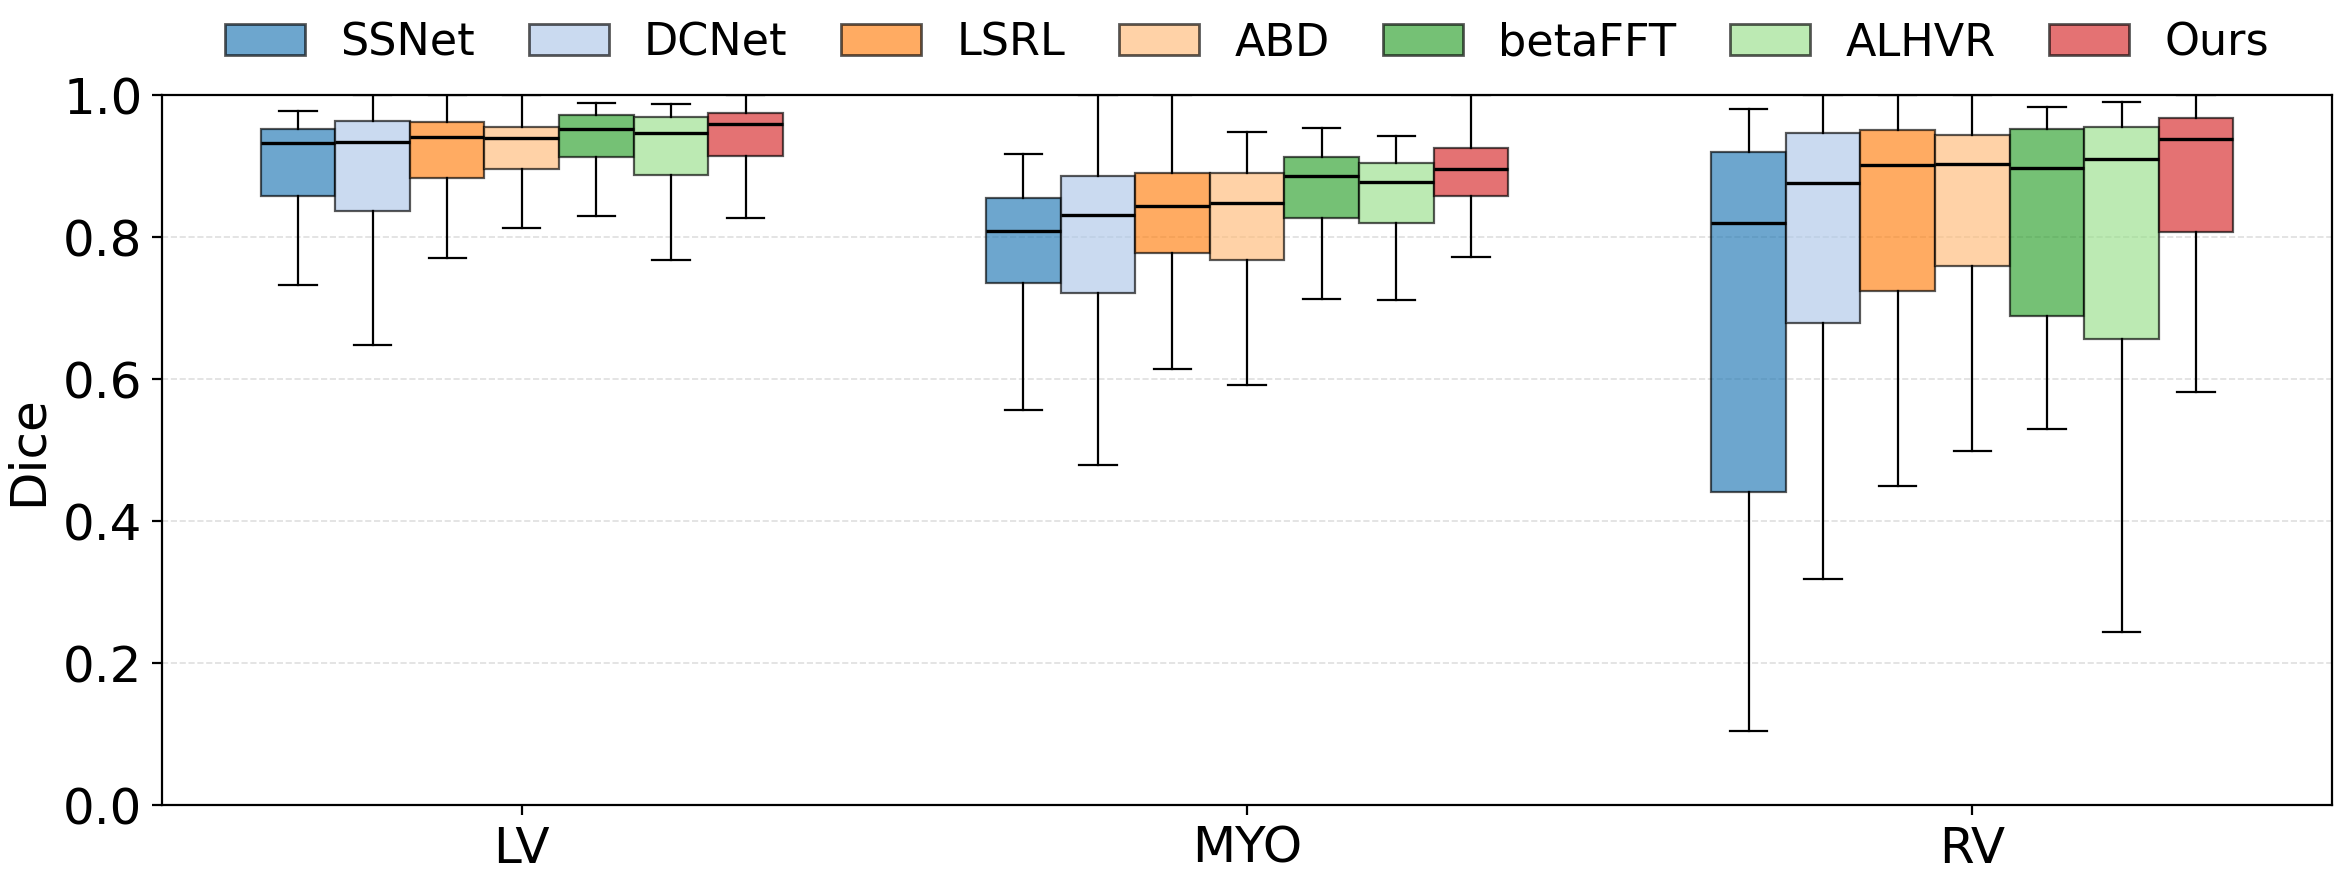
\includegraphics[width=0.8\linewidth]{Image/boxplotACDC.png}
  \caption{Dice boxplot comparison of different tissues between VGM-Seg and SSL methods on the ACDC dataset.}
  \label{ACDCboxplot}
\end{figure}



For the SCD, York, and ACDC datasets, SSL models are trained with 10\% labeled data, and our VGM-Seg consistently exceeds these methods, achieving average Dice improvements of 3.9\%, 11.6\%, and 6.5\%, respectively.
%
In particular, the improvement is most pronounced for the York dataset. The York dataset has only 33 patients, the 10\% labeled data provide very limited supervision, causing SSL methods to suffer significant performance degradation. In contrast, VGM-Seg maintains relatively stable predictive performance even without any labeled data, demonstrating its robustness under extreme label scarcity.


%这部分要换图分析
We visualize typical slices and their segmentation outputs, including input images, pseudo-colored masks, and overlaid predictive results. Qualitatively, VGM-Seg produces anatomically plausible and smooth contours in challenging apical and basal slices and shows robustness to noise and contrast variations. 
%
Moreover, 
Figure~\ref{ACDCboxplot} shows the boxplots of LV, MYO, and RV of different models in the ACDC dataset. 
It can be observed that segmentation accuracy is highest for the LV, followed by the RV, whose more flexible shape introduces moderate difficulty, while the MYO remains the most challenging structure to segment due to its thin, ring-like morphology.
%
Figure~\ref{fig:tsne} illustrates the t-SNE visualization of class features extracted by different models. %The results indicate that our VGM-Seg yields better inter-class separability.
%
It can be observed that our VGM-Seg achieves better inter-class separability and intra-class compactness compared to the other SSL methods.

\begin{figure}
    \centering
    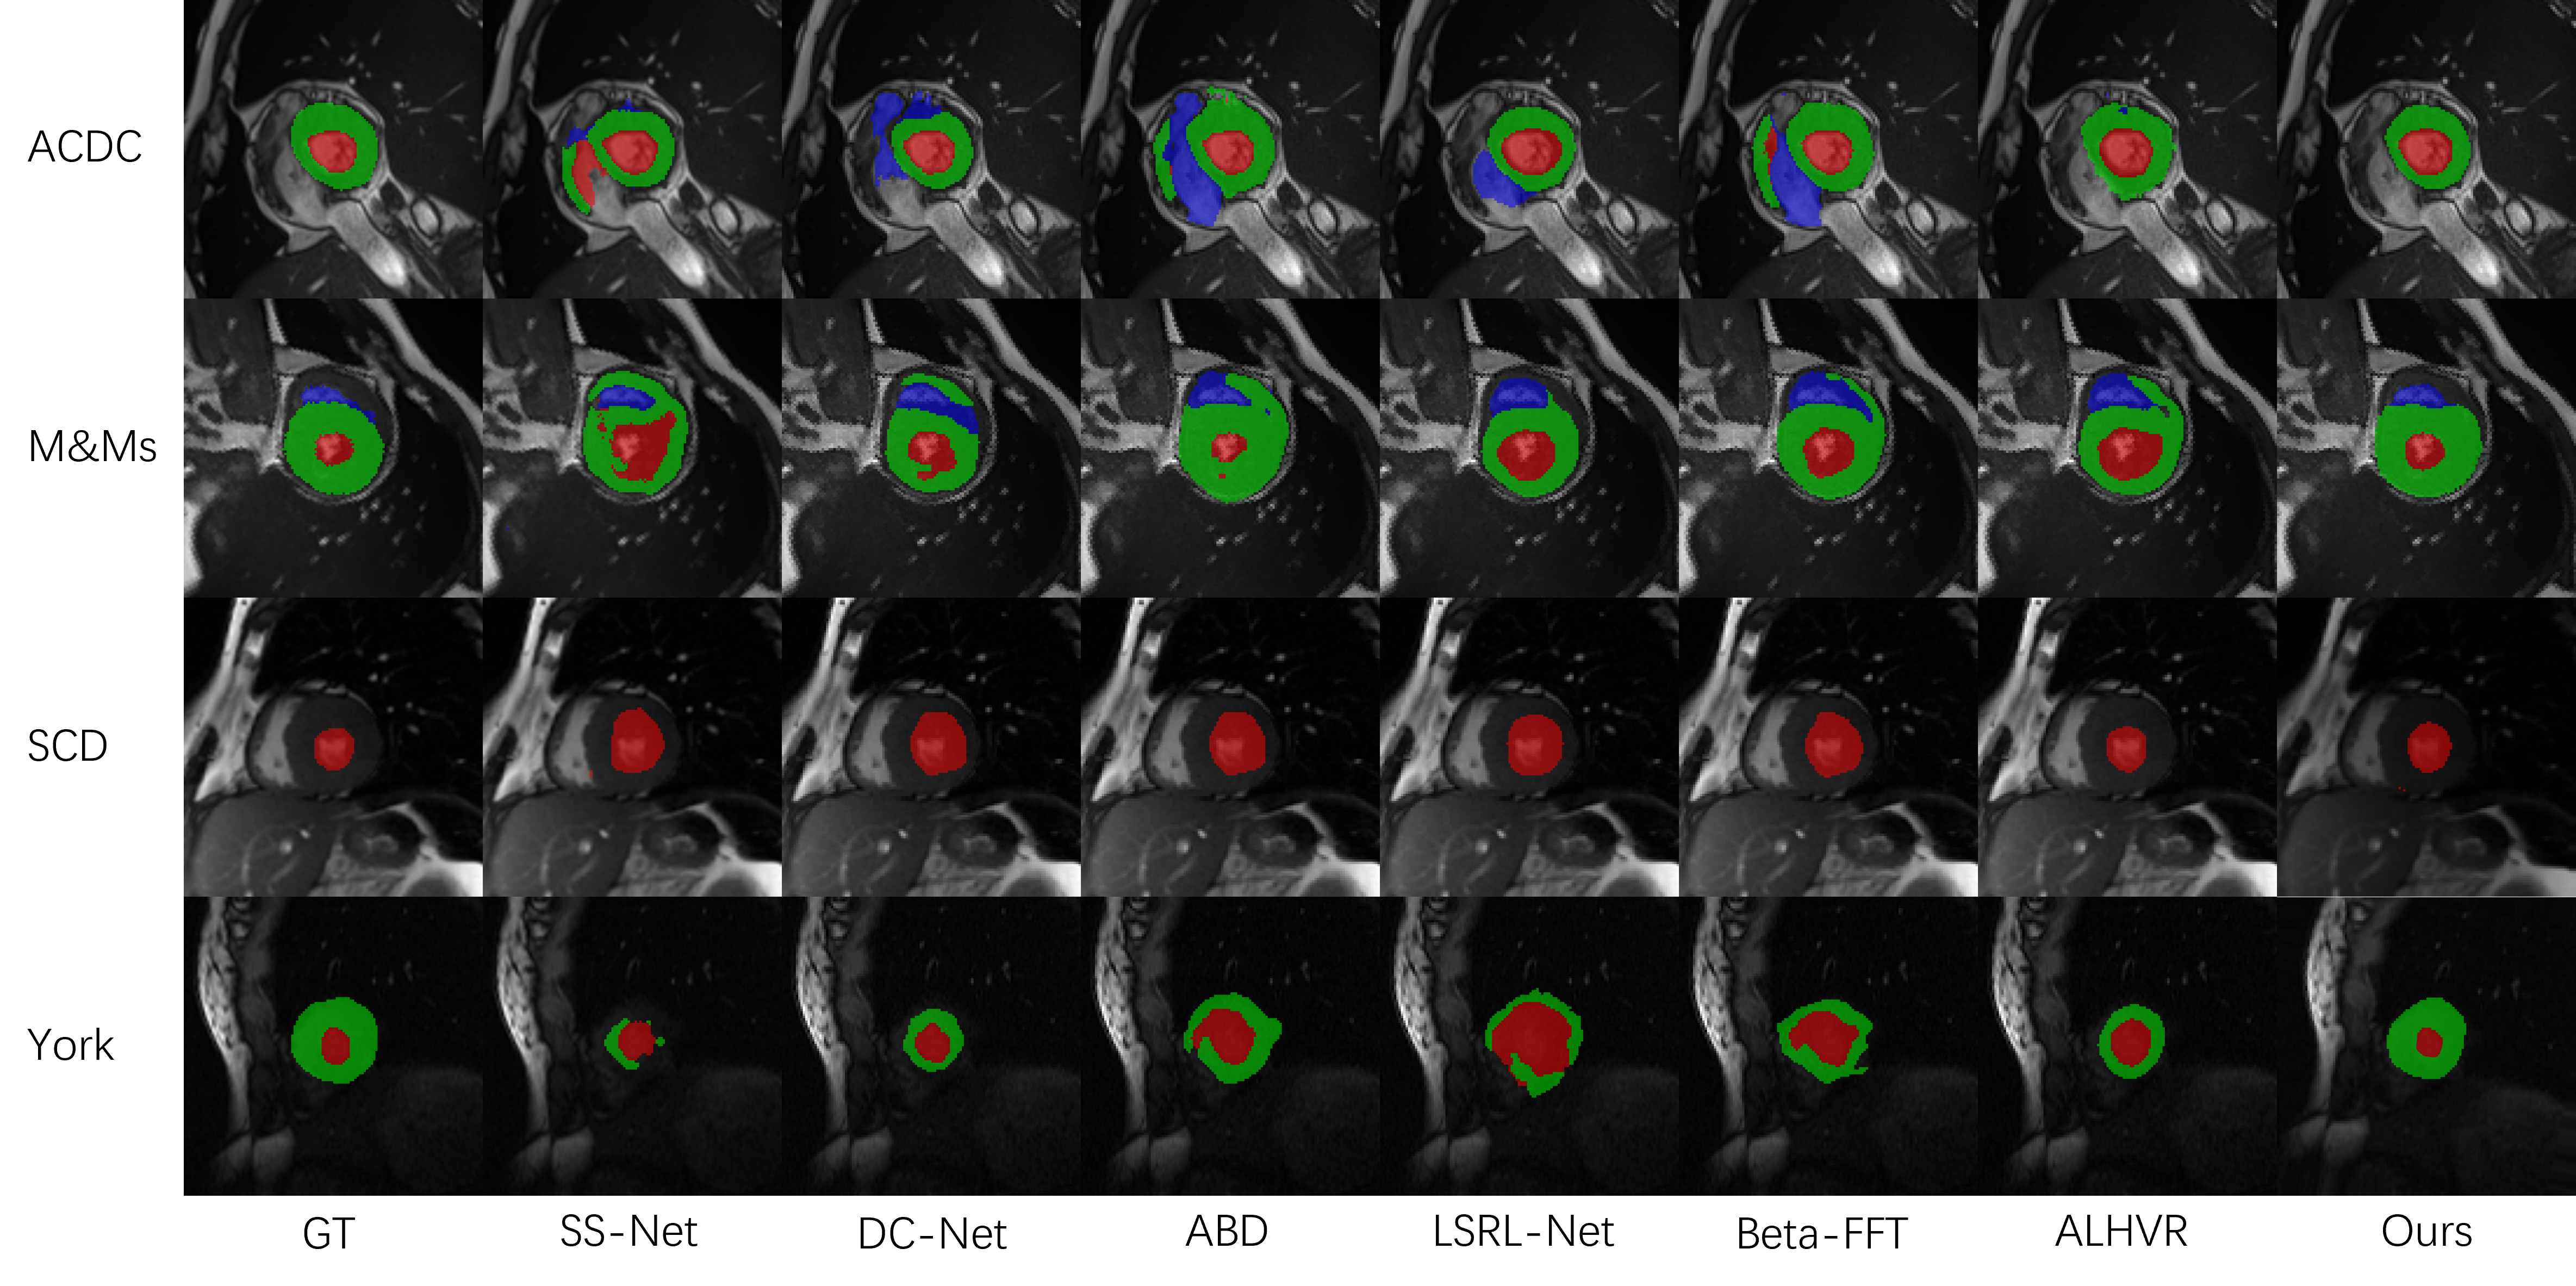
\includegraphics[width=1\linewidth]{Image/example.png}
    \caption{Demonstration of segmentation results using different models on four datasets.}
    \label{fig:placeholder}
\end{figure}



\begin{figure}
    \centering
    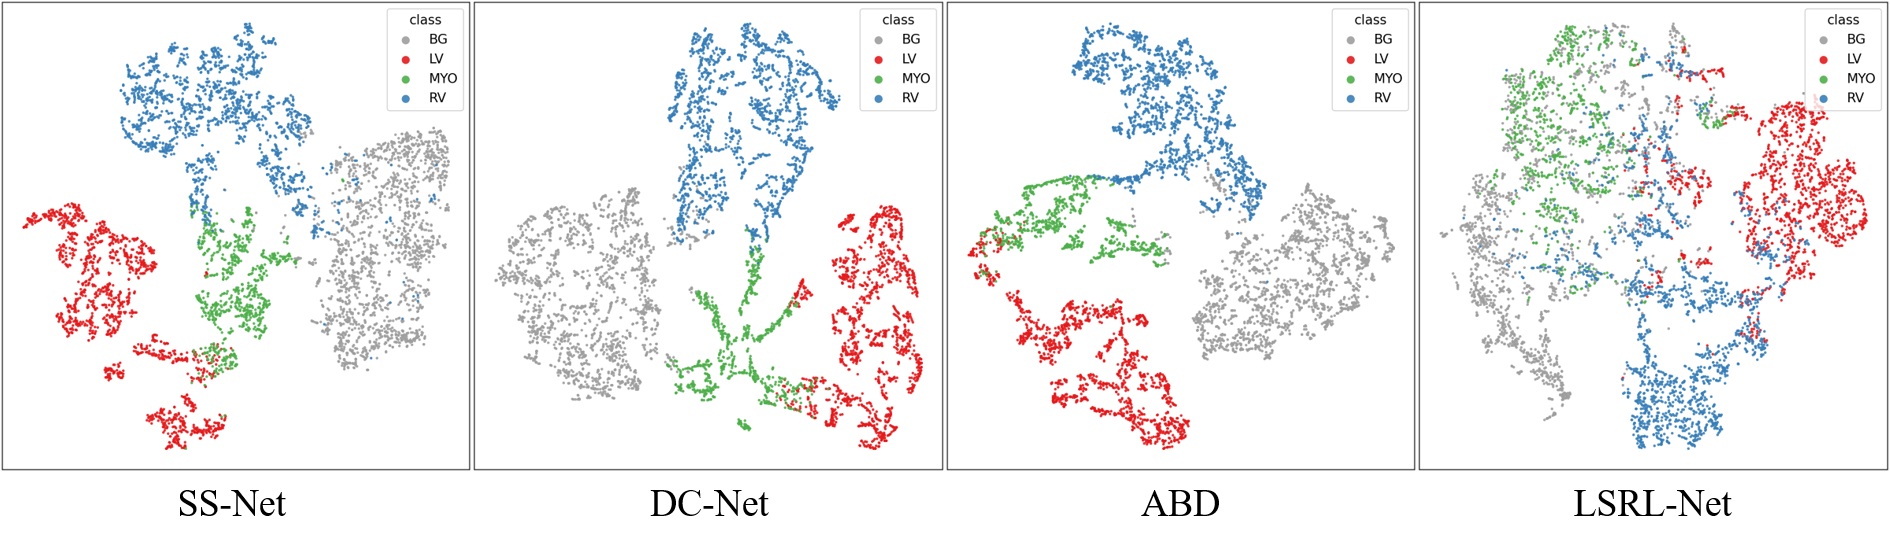
\includegraphics[width=1\linewidth]{Image/tsneSSL1.png}
    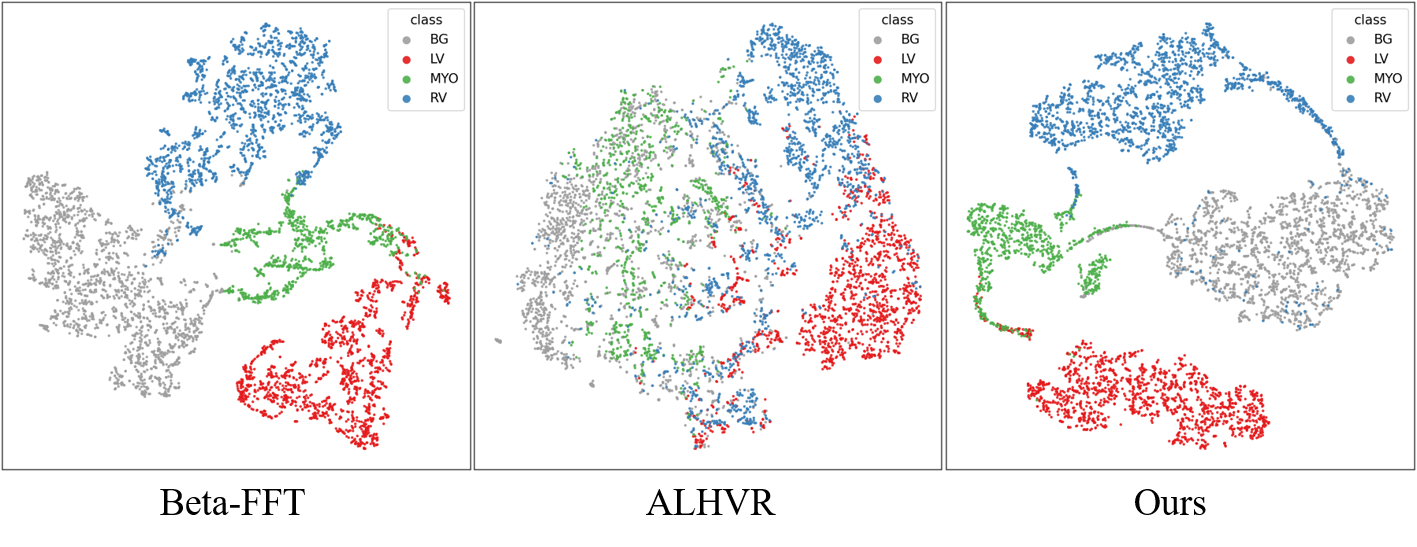
\includegraphics[width=0.75\linewidth]{Image/tsneSSL2.png}    
    \caption{t-SNE visualization of class-wise features extracted by different SSL models and our VGM-Seg.}
    \label{fig:tsne}
\end{figure}


\subsubsection{Comparison with Domain Adaptation Models}

In this experiment, we include state-of-the-art unsupervised domain adaptation (DA) methods for comparison. These DA methods leverage labeled source-domain data without target-domain annotations. 25\% of the ACDC data are used as the labeled source domain, and the M\&Ms, SCD, and York are used as the unlabeled target domains.
% 
To further show the single-source domain generalization ability of our VGM-Seg, our VGM-Seg is trained only on the ACDC dataset and directly evaluated on unseen target domains without any adaptation. We denote this model as VGM-Seg (DG).



Table~\ref{tab:domain_adaptation_results} lists the performance of VGM-Seg compared to other DA methods in the target domain. It should be emphasized that VGM-Seg is trained in the source and target domains, respectively, without any labeled data, while VGM-Seg (DG) is only trained in the source domain without labeled data, and the DA methods used 25\% ACDC labeled data in the source domain and unlabeled data in the target domain.
It is observed that VGM-Seg consistently outperforms DA methods in both the source and target domains in terms of all metrics.
It should be noted that the predictive performance of VGM-Seg in the source domain is independent of the target domain. Consequently, the accuracy of the source domain remains consistent across three different target domain datasets.
Interestingly, VGM-Seg (DG) also outperforms two DA methods, and its performance is close to that achieved by training directly in the target domain. This indicates that VGM-Seg has a strong cross-domain generalization capability. This observation is consistent with the analysis in Section~\ref{sec:DG}, suggesting that VGM-Seg behaves consistently with the Invariant Mechanism Assumption (IMA) in practice.

Figure~\ref{fig:DAcompare} shows the comparison of Dice boxplots using VGM-Seg and two DA methods in the source and target domains. It indicates that VGM-Seg achieves consistent performance in both domains, while the DA methods suffer from significant performance degradation or performance discrepancies compared to that on the source domain when applied to the target domain. 
This indicates that these DA methods are sensitive to domain shifts and cannot maintain consistent segmentation accuracy when transferred to the target domain.
Furthermore, Figure~\ref{fig:DAtsne} visualizes the t-SNE of the class-wise features extracted by the DA models and our VGM-Seg. It shows that both DA methods suffer from inter-class overlap in the source and target domains, especially for UDA-VAE++. By comparison, VGM-Seg maintains good inter-class separability across both domains.

% Table: Domain adaptation comparison (Source: ACDC(25%), Target: MM/SCD/YORK)
\begin{table*}[htbp]
\centering
\caption{Comparison with two domain adaptation methods using ACDC (25\%) as the labeled source domain and the unlabeled target domains.}
\label{tab:domain_adaptation_results}
\setlength{\tabcolsep}{5pt}
\renewcommand{\arraystretch}{1.2}
\begin{tabular}{c c c c c c c}
\toprule
\multirow{2}{*}{\makecell{Target\\Domain}} & 
\multirow{2}{*}{Method} & 
\multirow{2}{*}{Domain} &
\multicolumn{4}{c}{Metrics} \\
\cmidrule(lr){4-7}
 &  &  & Dice(\%)$\uparrow$ & Jaccard(\%)$\uparrow$ & HD95$\downarrow$ & ASD$\downarrow$ \\
\midrule
\multirow{5}{*}{MM}
 & \multirow{2}{*}{ODADA\cite{sun2022rethinking}}
 & Source & 82.31 & 75.47 & 7.46 & 2.14 \\
 &  & Target & 70.32 & 62.55 & 21.20 & 7.73 \\ \cline{2-7}
 & \multirow{2}{*}{UDA-VAE++\cite{lu2022unsupervised}}
 & Source & 66.63 & 55.72 & 57.55 & 2.97 \\
 &  & Target & 62.25 & 51.77 & 53.11 & 3.79 \\ \cline{2-7}
 & \multirow{2}{*}{Ours}
 & Source & \textbf{87.71} & \textbf{78.54} & \textbf{2.36} & \textbf{0.69} \\ 
 &  & Target & \textbf{83.85} & \textbf{71.41} & \textbf{2.50} & \textbf{0.76} \\ \cline{2-7}
  & Ours (DG)
 & Target & 82.08 & 70.43 & 2.76 & 0.85 \\ 		
\midrule
\multirow{5}{*}{SCD}
 & \multirow{2}{*}{ODADA\cite{sun2022rethinking}}
 & Source & 83.36 & 79.88 & 3.35 & 1.45 \\
 &  & Target & 81.87 & 70.77 & 8.26 & 4.29 \\ \cline{2-7}
 & \multirow{2}{*}{UDA-VAE++\cite{lu2022unsupervised}}
 & Source & 64.23 & 52.50 & 42.39 & 3.11 \\
 &  & Target & 79.89 & 69.06 & 14.10 & 2.90 \\ \cline{2-7}
 & \multirow{2}{*}{Ours}
 & Source & \textbf{87.71} & \textbf{78.54} & \textbf{2.36} & \textbf{0.69} \\
 &  & Target & \textbf{90.91} & \textbf{83.76} & \textbf{4.56} & \textbf{1.14} \\ \cline{2-7}
  & Ours (DG)
 & Target & 87.14 & 77.51 & 2.23 & 0.78 \\ 				
\midrule
\multirow{5}{*}{YORK}
 & \multirow{2}{*}{ODADA\cite{sun2022rethinking}}
 & Source & 82.47 & 77.01 & 4.05 & 1.62 \\
 &  & Target & 68.48 & 57.21 & 13.26 & 6.74 \\ \cline{2-7}
 & \multirow{2}{*}{UDA-VAE++\cite{lu2022unsupervised}}
 & Source & 67.89 & 56.57 & 40.89 & 3.48 \\
 &  & Target & 65.02 & 52.69 & 17.45 & 3.32 \\ \cline{2-7}
 & \multirow{2}{*}{Ours}
 & Source & \textbf{87.71} & \textbf{78.54} & \textbf{2.36} & \textbf{0.69}  \\
 &  & Target & \textbf{84.15} & \textbf{74.25} & \textbf{2.28} & \textbf{0.78} \\ \cline{2-7}
  & Ours (DG)
 & Target & 82.02 & 70.63 & 2.50 & 0.81 \\ 	
 			
\bottomrule
\end{tabular}
\end{table*}


\begin{figure}[htpb]
  \centering
  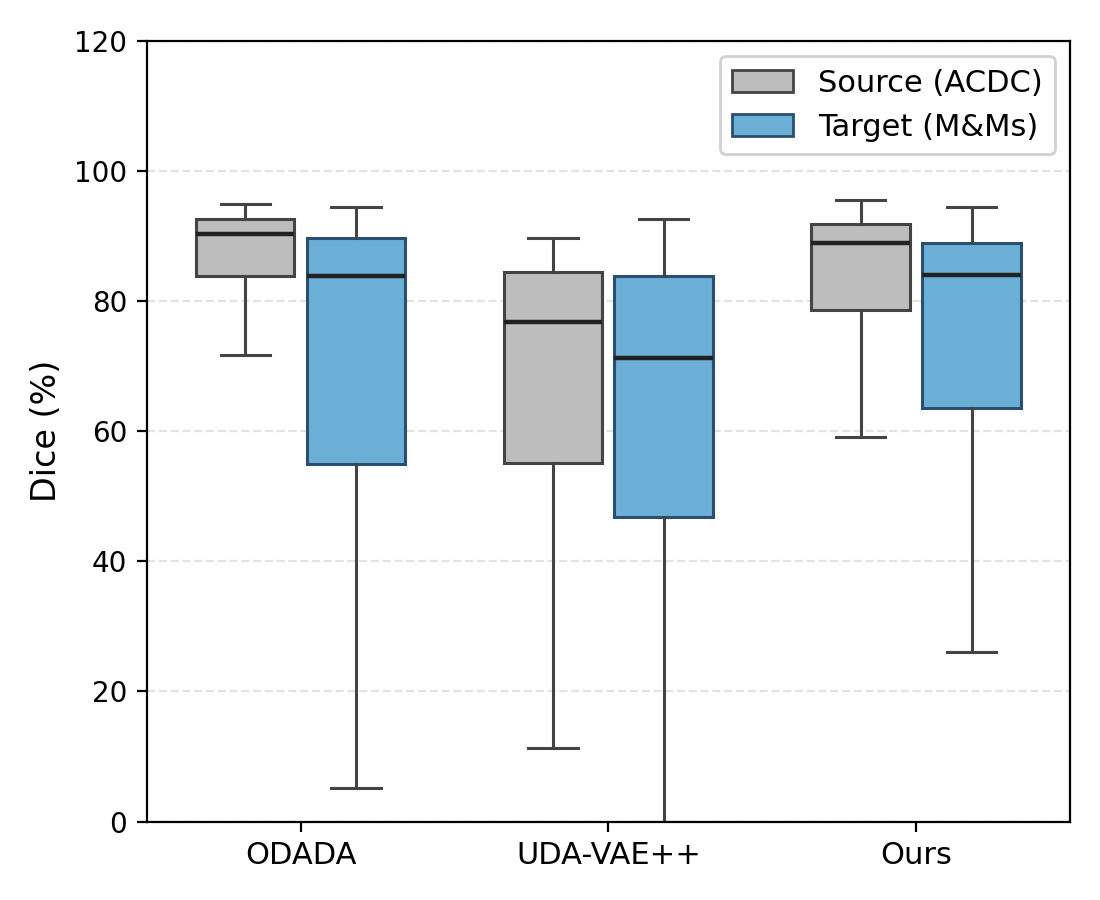
\includegraphics[width=0.3\linewidth]{Image/DAboxplotMM.png}
  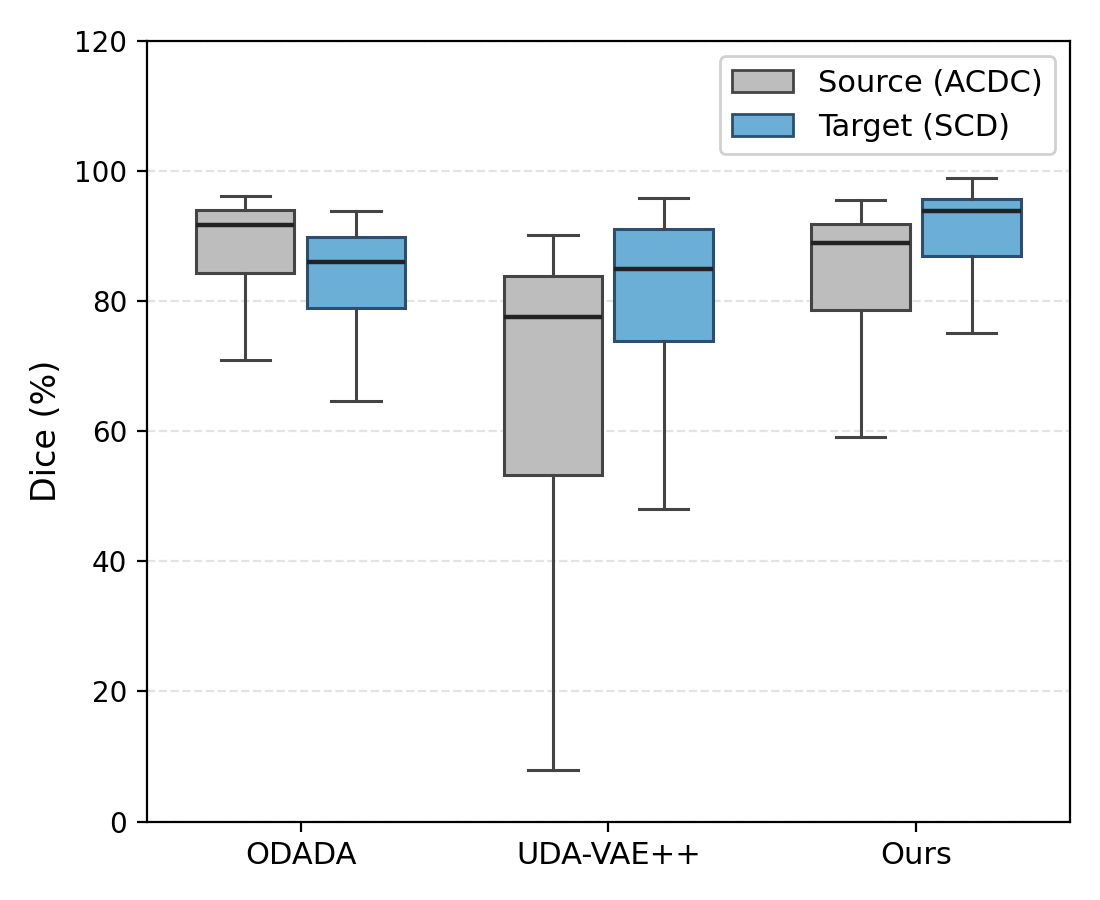
\includegraphics[width=0.3\linewidth]{Image/DAboxplotSCD.png}
  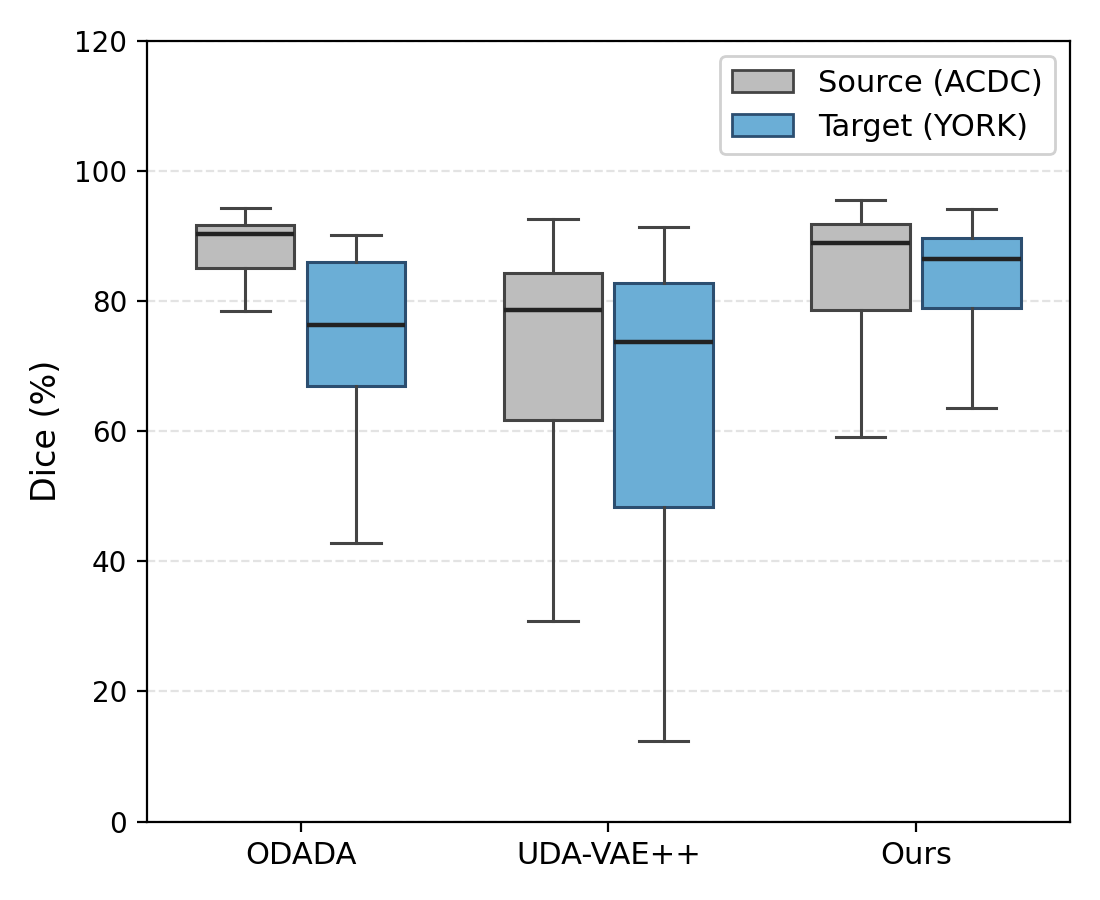
\includegraphics[width=0.3\linewidth]{Image/DAboxplotYork.png}
  \caption{Dice boxplot comparison between VGM-Seg and two DA methods on the source and target domains.}
  \label{fig:DAcompare}
\end{figure}



\begin{figure}[htpb]
  \centering
  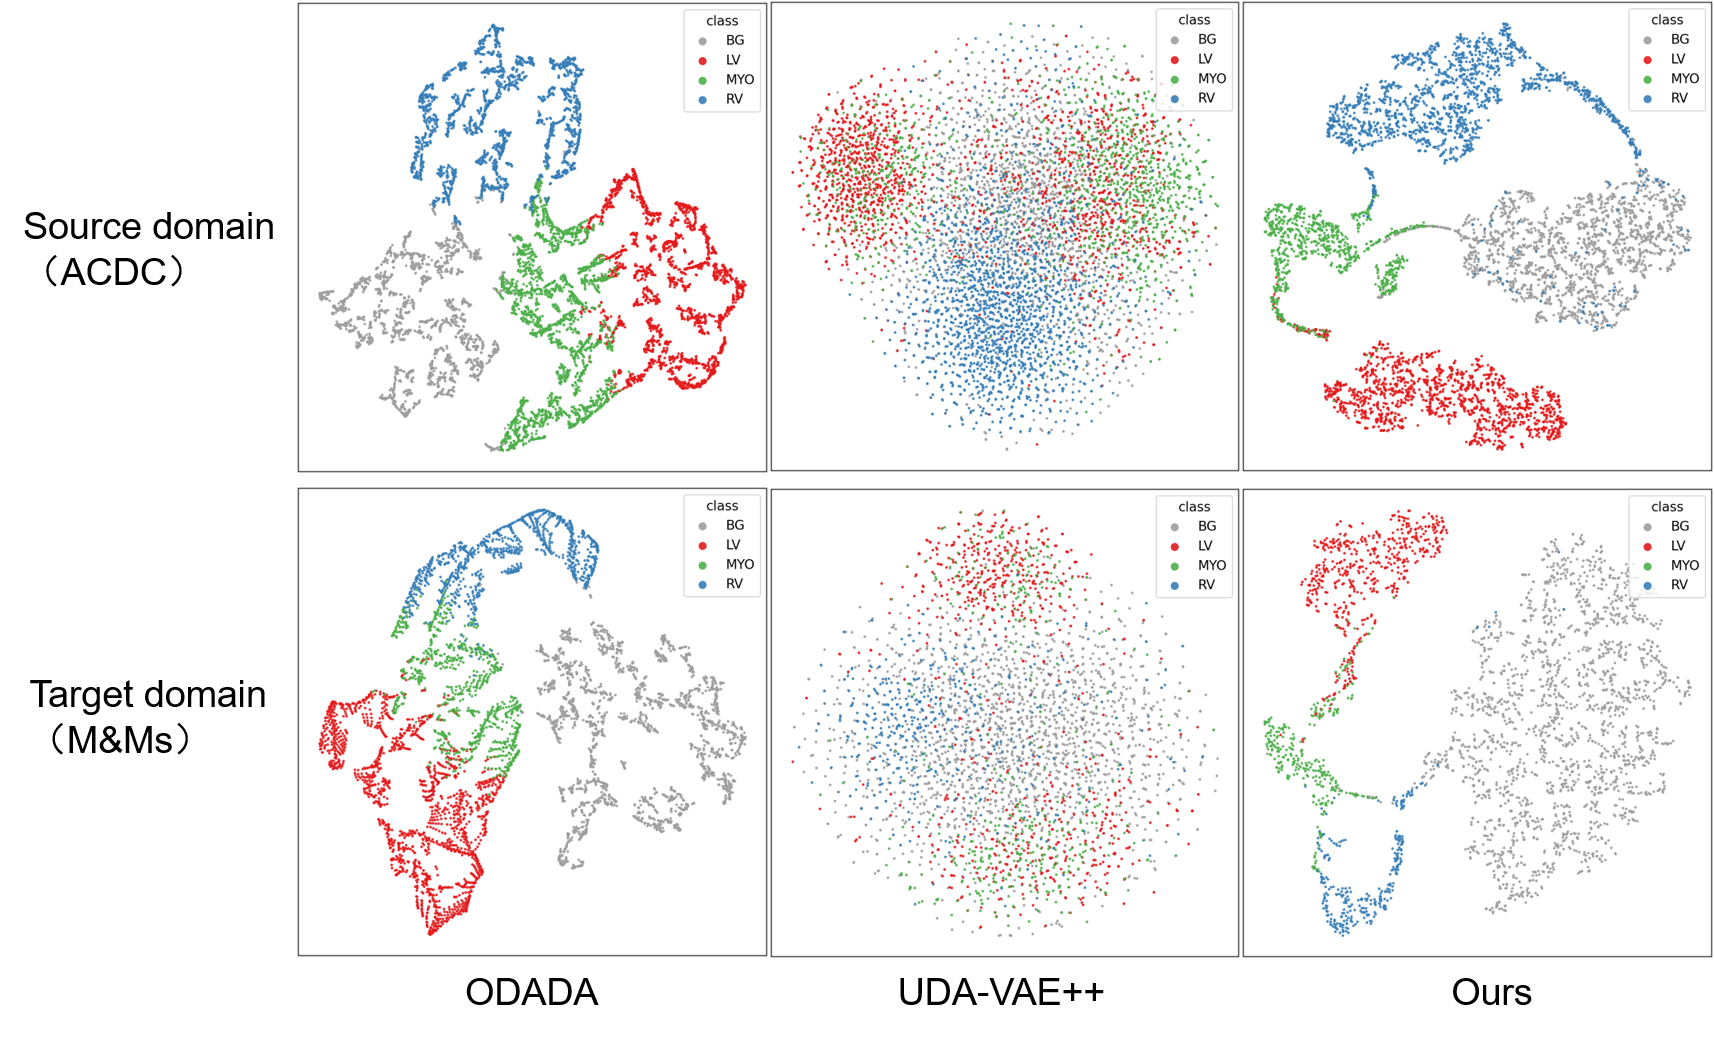
\includegraphics[width=0.9\linewidth]{Image/tsneDA.png}
  \caption{t-SNE visualization of class-wise features extracted by DA models and our VGM-Seg.}
  \label{fig:DAtsne}
\end{figure}




\subsection{Predictive Uncertainty}

Since the Gaussian mixture model is a probabilistic framework, it naturally provides pixel-wise uncertainty estimates through posterior assignment probabilities. For each pixel, the soft assignment distribution over the mixture components is obtained, and the uncertainty is quantified by the entropy of this distribution. Higher entropy values indicate ambiguous class assignments, which typically occur near anatomical boundaries or in regions with domain shifts.

%The concentration parameter of the Dirichlet distribution reflects confidence in the mixture weights.
%
We provide a qualitative comparison of entropy-based predictive uncertainty in representative slices of the target domain. Figure~\ref{fig:entropy_maps} shows the input image, ground truth, segmentation predictions, and the corresponding entropy maps for two DA methods and our VGM-Seg. 
In the entropy maps, VGM-Seg maintains relatively low and consistent uncertainty in both the source and target domains.



%这里补充一个小提琴图，统计四个数据集的不确定性比较（强调跨域不确定性的稳定性）
Figure~\ref{fig:violin} shows violin plots of the uncertainty distributions produced by different DA methods and our VGM-Seg in three target domains. Each sample in the plot represents the mean uncertainty of a single image.
It can be observed that on the three datasets, VGM-Seg produces less segmentation uncertainty than the other two DA methods. 
The reason may be attributed to the training strategies. DA methods typically rely on joint training with labeled source-domain data and unlabeled target-domain data, which attempt to bridge the source and target domains and introduce additional uncertainty due to the misalignment of the distributions of the two domains.
%While our VGM-Seg model captures intrinsic feature ambiguity through a probabilistic GMM while avoiding additional uncertainty introduced by cross-domain feature alignment. 
In contrast, VGM-Seg is trained independently on each domain and does not enforce cross-domain distribution alignment. The anatomical prior further regularizes the posterior distributions, leading to stable and confident predictions even in unseen domains. As a result, the uncertainty captured by VGM-Seg reflects primarily intrinsic segmentation ambiguity rather than alignment-induced uncertainty, leading to relatively lower uncertainty in the target domain.

\begin{figure}[t]
  \centering
  \includegraphics[width=\linewidth]{Image/entropy.png}
  \caption{Qualitative comparison of segmentation results and entropy-based predictive uncertainty on the source (top) and target (bottom) domains. From left to right: input image, ground-truth, prediction results, and uncertainty maps by UDA-VAE++, ODADA, and our VGM-Seg, respectively.}
  \label{fig:entropy_maps}
\end{figure}

\begin{figure}[t]
  \centering
  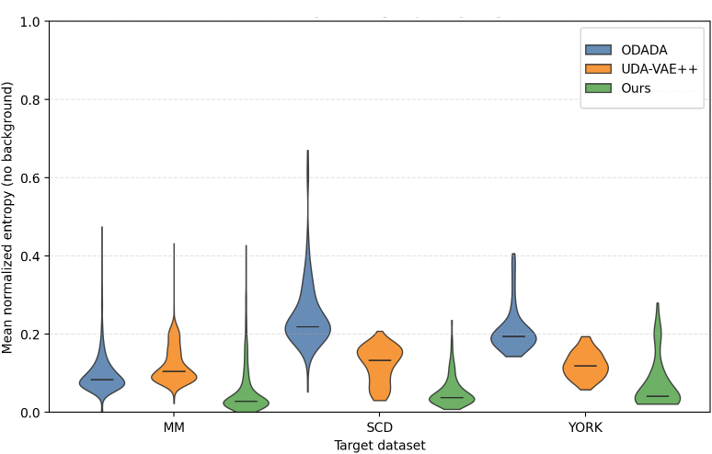
\includegraphics[width=0.6\linewidth]{Image/uncertainyDA.png}
  \caption{Violin plots of the segmentation uncertainty provided by UDA-VAE++, ODADA and our VGM-Seg, respectively, across three target domains.}
  \label{fig:violin}
\end{figure}

Furthermore, we perform segmentation uncertainty calibration to evaluate whether the predicted probabilistic confidence accurately reflects the true segmentation reliability. 
A well-calibrated model produces confidence estimates that are aligned with the true likelihood of correct predictions, which is critical for medical image analysis.



To plot the calibration curve, 
all pixels are partitioned into $B$ disjoint bins $\{\mathcal{B}_m\}_{m=1}^B$ according to their predictive class and confidence.
For each bin $\mathcal{B}_m$, the segmentation accuracy and the average confidence are computed as
\begin{equation}
\mathrm{acc}(\mathcal{B}_m) = \frac{1}{|\mathcal{B}_m|} \sum_{i \in \mathcal{B}_m} \mathbb{I}(\hat{y}_i = y_i),\qquad
\mathrm{conf}(\mathcal{B}_m) = \frac{1}{|\mathcal{B}_m|} \sum_{i \in \mathcal{B}_m} p^{max}_i,
\end{equation}
where $\hat{y}_i$, $y_i$ and $p^{max}_i$ are the prediction, the ground truth, and the maximum prediction probability of the $i$-th pixel, respectively; 
%$|\mathcal{B}_m|$ is the element number in $\mathcal{B}_m$. 
The calibration curve is obtained by plotting $\mathrm{acc}(\mathcal{B}_m)$ against $\mathrm{conf}(\mathcal{B}_m)$ for all bins, where the diagonal line indicates perfect calibration.
%
The Expected Calibration Error (ECE) is defined to quantitatively measure the calibration quality as
\begin{equation}
\mathrm{ECE} = \sum_{m=1}^{B} \frac{|\mathcal{B}_m|}{N} 
\left| \mathrm{acc}(\mathcal{B}_m) - \mathrm{conf}(\mathcal{B}_m) \right|,
\end{equation}
where $N$ is the total number of pixels.
A lower ECE value implies a better agreement between predictive confidence and accuracy.

Figure~\ref{fig:calibration} shows the uncertainty calibration curves and the ECE values of LSRL-Net, Beta-FFT and VGM-Seg in the ACDC and M\&Ms datasets. LSRL-Net and Beta-FFT were chosen as representative methods due to their competitive segmentation performance. It can be observed that VGM-Seg exhibits better uncertainty calibration performance with lower ECE values for the ACDC dataset. For the M\&Ms dataset, LSRL-Net achieves the lowest ECE, while our VGM-Seg is close to that of LSRL-Net and outperforms Beta-FFT with respect to ECE.

\begin{figure}[htpb]
    \centering
    \begin{subfigure}[t]{0.3\textwidth}
        \centering
        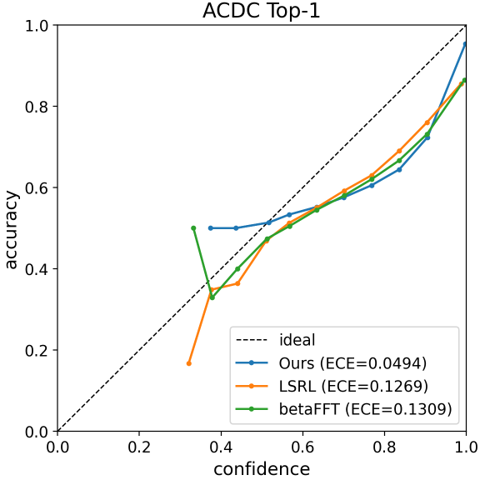
\includegraphics[width=\linewidth]{Image/calibrateACDC.png}
        \caption{ACDC}
    \end{subfigure}
    \hspace{0.01\textwidth}
    \begin{subfigure}[t]{0.3\textwidth}
        \centering
    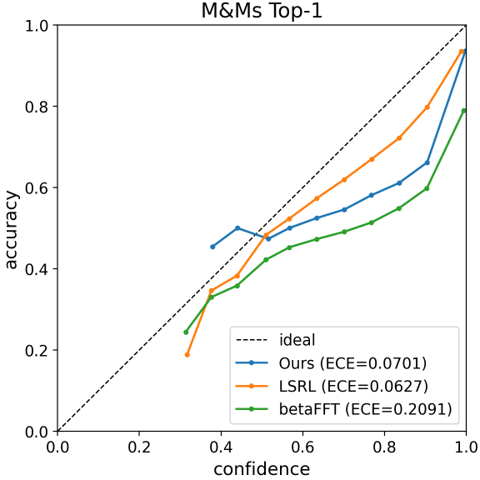
\includegraphics[width=\linewidth]{Image/calibrateMM.png}
        \caption{M\&Ms}
    \end{subfigure}
    \caption{Uncertainty calibration curves and ECE of different methods on two datasets.}
    \label{fig:calibration}
\end{figure}


% \begin{figure}[t]
%   \centering
%   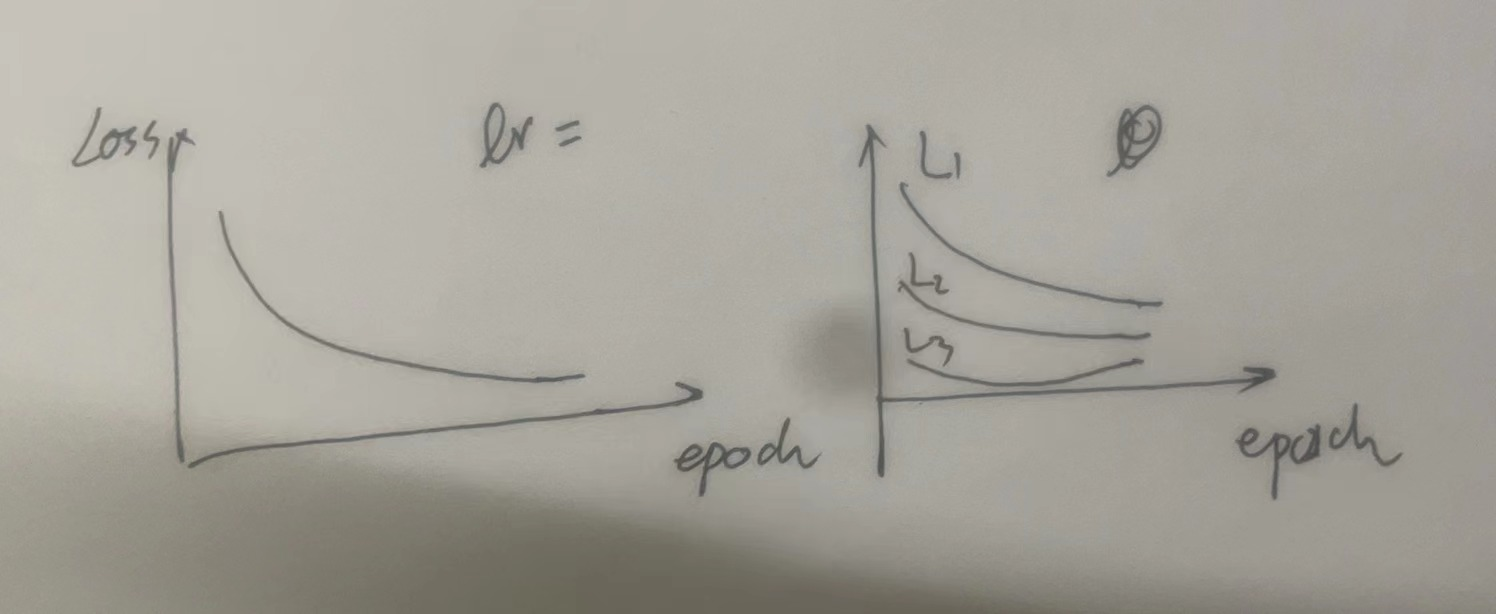
\includegraphics[width=\linewidth]{Image/loss.jpg}
%   \caption{Training loss convergence of VGM-Seg. Left: total loss of the overall framework. Right: loss curves of the three sub-networks.}
%   \label{fig:entropy_maps}
% \end{figure}


\subsection{Ablation Studies}
In this section, ablation experiments are performed to assess the influence of different components within VGM-Seg, including the dimensions of input features, the KL divergence term, the registration model, and the size of labeled data used for prior construction.
%
At first, we input image features of different dimensions into VGM-Seg to study their impact on performance.
Table~\ref{tab:ablation_dimension} lists the performance of our VGM-Seg with 4- and 16-dimensional features, respectively. It can be seen that using 4-dimensional features, more stable predictive results can be obtained. 
The reason may be that the 4-dimensional features represent semantic abstractions derived by the feature extractor $\mathbf{E}$ for the segmentation classes. As highly abstracted representations, they are less sensitive to fine-grained details, leading to a more stable construction of GMM. This stability is also reflected in the improved HD95 and ASD metrics.

Secondly, we remove the KL divergence term from the loss in Eq.\eqref{loss_total} to evaluate its regularization effect on VGM-Seg. 
Table~\ref{tab:ablation_KL} lists the performance of VGM-Seg with and without the KL divergence term. The results show that the KL divergence term clearly improves the predictive results by regularizing the components of the Gaussian mixture.

% Table 5: Component ablation
\begin{table}[htbp]
  \centering
  \caption{Ablation study on the effect of different input feature dimensions on the York dataset.}
  \begin{tabular}{l c c c c}
    \toprule
    	Dimension & Dice(\%)$\uparrow$ & Jaccard(\%)$\uparrow$ & HD95$\downarrow$ & ASD$\downarrow$ \\
    \midrule
    4 & \textbf{84.15} & \textbf{74.25} & \textbf{2.28 } & \textbf{0.78} \\
    16  & 84.02 & 73.72 & 3.30 & 1.31 \\
    \bottomrule
  \end{tabular}
  \label{tab:ablation_dimension}
\end{table}

% Table 5: Component ablation
\begin{table}[htbp]
  \centering
  \caption{Ablation study on the effect of the KL divergence term on the York dataset.}
  \begin{tabular}{l c c c c}
    \toprule
    	KL & Dice(\%)$\uparrow$ & Jaccard(\%)$\uparrow$ & HD95$\downarrow$ & ASD$\downarrow$ \\
    \midrule
    $\checkmark$ & \textbf{84.15} & \textbf{74.25} & \textbf{2.28} & \textbf{0.78} \\
      & 80.14 & 72.63 & 3.49 & 1.12 \\
    \bottomrule
  \end{tabular}
  \label{tab:ablation_KL}
\end{table}

Next, we remove the registration module to perform VGM-Seg. As listed in Table~\ref{tab:ablation_components}, the registration module is important in aligning the predicted weights to the Dirichlet anatomical prior.
Finally, we evaluated the influence of the size of the labeled dataset on the construction of the Dirichlet anatomical prior.
We vary the size of the labeled dataset used to construct the Dirichlet anatomical prior, while keeping all other settings fixed. Table~\ref{tab:ablation_prior_size} indicates that increasing the size of the labeled dataset is beneficial for improving the accuracy of the prediction. Also, it can be seen that our VGM-Seg is not sensitive to the size of the labeled dataset.

% Table 5: Component ablation
\begin{table}[htbp]
  \centering
  \caption{Ablation study on the effect of registration model on the M\&Ms dataset.}
  \begin{tabular}{c c c c c}
    \toprule
		Registration &  Dice(\%)$\uparrow$ & Jaccard(\%)$\uparrow$ & HD95$\downarrow$ & ASD$\downarrow$ \\
    \midrule
    $\checkmark$ & \textbf{83.85} & \textbf{71.41}  & \textbf{2.50} & \textbf{0.76} \\
     & 73.19 & 59.05 & 4.55 & 1.06 \\
    \bottomrule
  \end{tabular}
  \label{tab:ablation_components}
\end{table}



% Table 6: Prior size ablation
\begin{table}[htbp]
  \centering
  \caption{Effect of auxiliary labeled set size for building the Dirichlet anatomical prior. Evaluation is performed on the M\&Ms dataset. }
  \begin{tabular}{c c c c c}
    \toprule
    ACDC subset & Dice(\%)$\uparrow$ & Jaccard(\%)$\uparrow$ & HD95$\downarrow$ & ASD$\downarrow$ \\
    \midrule
    5\%  & 82.36 & 70.82 & 2.58 & 0.76 \\
    10\% & 82.82 & 71.56 & 2.58 & 0.77 \\
    25\% & \textbf{83.85} & \textbf{71.41} & \textbf{2.50} & \textbf{0.76} \\
    \bottomrule
  \end{tabular}
  \label{tab:ablation_prior_size}
\end{table}

% \paragraph{Conclusion from ablations.}
% Overall, the ablations support two conclusions: (i) explicit anatomical priors are a key driver of stable label-free adaptation, and (ii) alignment (registration) is necessary to make the prior effective under field-of-view and scale differences; otherwise performance drops and boundary errors increase. In addition, enlarging the auxiliary labeled subset improves the prior quality but exhibits diminishing returns beyond a moderate size.


\subsection{Computational Cost}
%不同模型epoch时间比较

Table~\ref{tab:cost} lists the computational time of each epoch using different models during training. It can be observed that VGM-Seg requires a relatively longer training time and a large number of parameters. This is mainly because VGM-Seg consists of three sub-networks, and jointly training these sub-networks increases the overall training cost. 


\begin{table}[htpb]
    \centering
    \begin{tabular}{c|c|c}
    \toprule
  Methods & Time(s)/epoch & Params (M)\\
\hline
DeepSVG	& 90  &  7.24\\ 
SS-Net	& 27 & 1.83\\ 
DC-Net	& 26 & 2.58\\ 
ABD	& 96  & 3.66\\ 
LSRL-Net	& 78  & 1.94\\ 
Beta-FFT	& 74  & 3.66\\ 
ALHVR	& 68  & 3.63\\ 
ODADA(DA)	& 30  & 60.57\\ 
UDA-VAE++(DA)	& 45  & 8.43\\ 
Ours	& 120 & 93.17\\ 
\bottomrule
    \end{tabular}
  \caption{Comparison of training efficiency and parameter count across different models. }
    \label{tab:cost}
\end{table}


\section{Conclusion}
We propose VGM-Seg, an unsupervised cardiac segmentation framework that integrates a pixel-wise Gaussian mixture model into a variational inference framework. By explicitly modeling class-conditional feature distributions and incorporating an anatomical prior, VGM-Seg provides a principled probabilistic formulation for cardiac segmentation without requiring manual annotations. Benefiting from the variational GMM and prior-guided regularization, VGM-Seg outperforms traditional GMM-based methods, semi-supervised approaches with limited labeled data, and domain-adaptation methods. In particular, our VGM-Seg demonstrates a good cross-domain generalization, stable performance across different datasets, and well-calibrated uncertainty estimation, highlighting its robustness and practical applicability.


Future work will investigate more flexible variational distributions beyond Gaussian mixtures to better capture complex feature structures and further enhance uncertainty quantification.
%% The Appendices part is started with the command \appendix;
%% appendix sections are then done as normal sections
% \appendix
% \section{Example Appendix Section}
% \label{app1}

% Appendix text.



\bibliographystyle{elsarticle-num} 
\bibliography{refs}

\end{document}


